\documentclass[a4paper]{report}

\input{setup/preamble}
\input{setup/macros}
\input{setup/letterfonts}

\addbibresource{gr.bib} 

\course{Econometrics II}
\professor[https://markomlikota.github.io/]{Marko Mlikota}
\me[jingle.fu@graduateinstitute.ch]{}
\institute{Graduate of International and Developoment Studies, Geneva}
\class{International Economics}
\session{Semester II, 2024}
\date{Based on lectures by \profloc{} in Spring semester, 2025
% \\ Notes created by Mubtasim Fuad 
\\~\\ Draft updated on \today}

\begin{document}

\renewcommand\thepage{Title}
\maketitle
\renewcommand\thepage{Preface} 
% \chapter*{Preface}  % to show preface on toc
\begin{myminipage} 
     This is the lecture note taken in the course \textit{\courseloc} taught by \profloc{} at \instituteloc{} as part of the \classloc{} program (\sessionloc).
     
     Currently, these are just drafts of the lecture notes. There can be typos and mistakes anywhere. So, if you find anything that needs to be corrected or improved, please inform at \myemailloc. \bigskip

     % I am deeply grateful to my late friend, Gilles Castel, who introduced me to \LaTeX{} for the first time.
\end{myminipage}

% \addcontentsline{toc}{chapter}{\protect\numberline{}Preface} % to show preface on toc
\pagenumbering{gobble}
% \pagenumbering{roman}   % to show preface on toc
\newpage
\pagestyle{plain}
\pagenumbering{roman}
\pdfbookmark{\contentsname}{toc}              
\setcounter{tocdepth}{3}
\tableofcontents
\newpage
\pagestyle{head}
\pagenumbering{arabic}

% start lectures
\chapter{Review of Econometrics I}
\section{Introduction}

\begin{definition}[Proportional Function]
    We say $f(x)$ is proportional to $g(x)$ if there exists a constant $c$,
    such that $f(x) = c \cdot g(x)$ for all $x$ in the domain of interest.
    We denote this relationship as $f(x) \propto g(x)$.
\end{definition}

If $y$ is a R.V. with pdf $f(y) \propto \exp(-\lambda y)$ for $y \geq 0$ and $0$ otherwise,
then we know $f(y) = c \cdot \exp(-\lambda y)$.
To find $c$, we use the fact that the total probability must equal 1:
\begin{equation}
    \int_0^\infty f(y) dy = 1 \implies \int_0^\infty c \cdot \exp(-\lambda y) dy = 1
\end{equation}
Calculating the integral, we have:
\begin{equation}
    c \cdot \left[ -\frac{1}{\lambda} \exp(-\lambda y) \right]_0^\infty = 1
\end{equation}
Evaluating the limits, we get:
\begin{equation}
    c = \lambda 
\end{equation}

Now looking at the normal distribution: $y \sim \mathcal{N} \left( \mu , \sigma^2 \right)$
we have
\begin{align}
    p(y | \mu, \sigma^2) &= \frac{1}{\sqrt{2 \pi \sigma^2}} \exp \left( -\frac{(y - \mu)^2}{2\sigma^2} \right) \\
    & \propto \exp \left( -\frac{1}{2\sigma^2} (y - \mu)^2 \right)
\end{align}

For a simple linear regression model $y_i = \theta + u_i$, where $\mathbb{E}[ u_i | \theta =0]$,
we know $\mathbb{E}[ y_i | \theta ] = \theta$.



\begin{itemize}
    \item Least-squares estimator:
    \begin{align}
        \hat{\theta}_{LS} &= \arg \min_\theta \sum_{i=1}^n (y_i - \mathbb{E}[ y_i | \theta ])^2 \\
        &= \arg \min_\theta \left( y_i - \theta \right)^2 \\
        &= \frac{1}{n} \sum_{i=1}^n y_i
    \end{align}
    \item Maximum likelihood estimator(Assuming $y_i | \theta \sim \mathcal{N} \left( \theta , \sigma^2 \right)$):
    \begin{align}
        \hat{\theta}_{ML} &= \arg \max_\theta \prod_{i=1}^n p(y_i | \theta) \\
        &\propto \arg \max_\theta \prod_{i=1}^n \exp \left( -\frac{1}{2\sigma^2} (y_i - \theta)^2 \right) \\
        &\propto \arg \min_\theta \sum_{i=1}^n (y_i - \theta)^2 \\
        &= \frac{1}{n} \sum_{i=1}^n y_i = \hat{\theta}_{LS}
    \end{align}
    It's easy to see that:
    \begin{align}
        \mathbb{E}[\hat{\theta } | \theta ] &= \mathbb{E} \left[ \frac{1}{n} \sum_{i=1}^n y_i | \theta \right] = \theta \\
        \mathbb{V}[\hat{\theta } | \theta ] &= \mathbb{V} \left[ \frac{1}{n} \sum_{i=1}^n y_i | \theta \right] = \frac{\sigma^2}{n}
    \end{align}
    Even without assuming that $\hat{\theta } | \theta \sim \mathcal{N} \left( \theta , \frac{\sigma^2}{n} \right)$,
    we know by the Central Limit Theorem that:
    \begin{equation}
        \sqrt{n} \left( \hat{\theta } - \theta \right) \xrightarrow{d} \mathcal{N} \left( 0 , \sigma^2 \right) \Rightarrow \hat{\theta } | \theta \sim \mathcal{N} \left( \theta , \frac{\sigma^2}{n} \right)
    \end{equation}
\end{itemize}

\begin{definition}[Posterior]
    The posterior distribution of a parameter $\theta$ given data $y$ is defined as:
    \begin{equation}
        p(\theta | y) = \frac{p(y | \theta) p(\theta)}{p(y)} \propto p(y | \theta) p(\theta)
    \end{equation}
    where $p(y | \theta)$ is the likelihood, $p(\theta)$ is the prior distribution of $\theta$, and $p(y)$ is the marginal likelihood.

    This shows how, given a prior belief about $\theta$ and observed data $y$,
    we can update our belief to form the posterior distribution.
\end{definition}

\begin{eg}
    Taking a simple example: 
    \begin{equation}
        y_i | \theta \sim \mathcal{N} \left( \theta , 1 \right) \Rightarrow p(y_i | \theta) = \frac{1}{\sqrt{2\pi}} \exp \left( -\frac{1}{2} (y_i - \theta)^2 \right)
    \end{equation}
    Suppose $\theta \sim \mathcal{N} \left( \theta , \frac{1}{\lambda } \right)$.
    \begin{align}
        p(\theta | y) & \propto p(y | \theta) p(\theta) \\
        &= (2\pi )^{ -\frac{n}{2}} \exp \left( -\frac{1}{2} (y_i - \theta)^2 \right) \cdot \frac{1}{\sqrt{2\pi \frac{1}{\lambda}}} \exp \left( -\frac{1}{2 \frac{1}{\lambda }} (\theta - \theta_0)^2 \right) \\
        & \propto \exp \left( -\frac{1}{2} \sum_{i=1}^n (y_i - \theta)^2 - \frac{\lambda }{2} (\theta - \theta_0)^2 \right) \\
        & \propto \exp \left( -\frac{1}{2} \left[ (n + \lambda ) \theta^2 - 2 \left(\sum_{i=1}^n y_i + \lambda \theta_0\right) \theta \right] \right) \\
        \theta | y & \sim \mathcal{N} \left( \frac{1}{n + \lambda } \left( \sum_{i=1}^n y_i + \lambda \theta_0 \right), \frac{1}{n + \lambda } \right)
    \end{align}
    We guess that $\theta | y \sim \mathcal{N} \left( \bar{\theta }, \bar{V} \right)$,
    then we can write:
    \begin{align}
        p \left( \theta | y \right) & \propto \exp \left( -\frac{1}{2} \bar{V}^{-1} (\theta - \bar{\theta })^2 \right) \\
        & \propto \exp \left( -\frac{1}{2} \left[ \bar{V}^{-1} \theta^2 - 2 \bar{V}^{-1} \bar{\theta } \theta \right] \right)
    \end{align}
    then, we know that:
    \begin{equation}
        \bar{V}^{-1} = n + \lambda 
    \end{equation}
    and
    \begin{align}
        \bar{\theta } &= \frac{1}{n + \lambda } \left( \sum_{i=1}^n y_i + \lambda \theta_0 \right) \\
        &= \frac{1}{n + \lambda } \cdot \left[ n \cdot \sum_{i=1}^n y_i + \lambda\, \theta_0 \right] \\
        & \to \begin{cases}
            \theta_0, &\text{ if } \lambda \to \infty ; \\
            \hat{\theta }, &\text{ if } \lambda \to 0 \text{ and/or } n \to \infty .
        \end{cases}
    \end{align}
    In general, we can push $\theta _0$ to $0$ by re-centering $y_i$.
    Then we have:
    \begin{equation}
        \hat{\theta } = \frac{n}{n + \lambda }\, \underset{ \hat{\theta }_{ML} }{ \underbrace{ \frac{1}{n} \sum_{i=1}^n y_i }}
    \end{equation}
    then,
    \begin{align}
        \mathbb{E}[\hat{\theta } | \theta ] &= \mathbb{E}\left[ \frac{1}{n + \lambda} \sum_{i=1}^n y_i | \theta \right] \\
        &= \frac{1}{n + \lambda} \sum_{i=1}^n \mathbb{E}[y_i | \theta ] = \frac{1}{n + \lambda} \sum_{i=1}^n \theta = \frac{n}{n + \lambda} \theta 
    \end{align}
    for any $\lambda > 0$, this $\hat{\theta }$ is biased.
    \begin{align}
        \mathbb{V}[\hat{\theta } | \theta ] &= \mathbb{V}\left[ \frac{1}{n + \lambda} \sum_{i=1}^n y_i | \theta \right] \\
        &= \frac{1}{(n + \lambda)^2} \sum_{i=1}^n \mathbb{V}[y_i | \theta ] \\
        &= \frac{n}{(n + \lambda)^2} \\
        &< \frac{1}{n} = \mathbb{V}[\hat{\theta }_{ML} | \theta ] \text{ for any } \lambda > 0.
    \end{align}
\end{eg}

\section{Hypothesis Testing}

We want to test $H_0: \theta = 0$ vs $H_1: \theta \neq 0$.
$\varphi \in \{0, 1\}$ is a test function, where $\phi = 1$ means accept,
then the size of the test is defined as:
\begin{equation}
    \alpha = \mathbb{P}(\varphi = 1 | \theta = 0) = \mathbf{1} \{\theta < \theta_0 \}
\end{equation}

We have:
\begin{align}
    \mathbb{P}(\theta | y) \begin{dcases}
        p\left( \theta \in \Theta_0 | y \right);\\
        p\left( \theta \notin \Theta_0 | y \right) = 1 - p\left( \theta \in \Theta_0 | y \right).
    \end{dcases}
\end{align}
Then, the posterior odds ratio is defined as:
\begin{equation}
    \frac{p\left( \theta \in \Theta_0 | y \right)}{p\left( \theta \in \Theta_1 | y \right)} = \frac{p\left( \theta \in \Theta_0 | y \right)}{1 - p\left( \theta \in \Theta_0 | y \right)}
\end{equation}
The Bayes factor is defined as:
\begin{equation}
    BF = \frac{\text{Post. Odds}}{\text{Prior Odds}}
\end{equation}

\begin{eg}
    
Suppose $\theta \in \{0, 1\}$, and $y | \theta \in \{ 0,1,2,3,4 \}$,
\begin{table}[H]
    \centering
    \begin{tabular}{c|ccccc}
        \toprule
         & 0 & 1 & 2 & 3 & 4 \\
        \midrule
        $p(y | \theta = 0)$ & 75\% & 14\% & 4\% & 3.7\% & 3.3\% \\
        $p(y | \theta = 1)$ & 70\% & 25.1\% & 4\% & 0.5\% & 0.4\% \\
        \bottomrule
    \end{tabular}
    \caption{Example}
    \label{tab:example}
\end{table}

Suppose $y=2$, then the hypothesis test results are:
\begin{align}
    \mathcal{H}_0: \theta = 0 & \to p(y \geq 2 | \theta = 0) = 11\% \\
    \mathcal{H}_1: \theta = 1 & \to p(y \geq 2 | \theta = 1) = 4.9\%
\end{align}

The Bayes factors are:
\begin{align}
    BF &= \frac{p\left(\theta = 1 | y = 2 \right)}{p\left(\theta = 0 | y = 2 \right)} \\
    &= \frac{p(y = 2 | \theta = 1)p(\theta = 1)}{p(y = 2 | \theta = 0)p(\theta = 0)}
\end{align}

\end{eg}

Consider $c(y)$ such that $\mathbb{P}\left[ \theta \in c(y) | \theta \right] = 1- \alpha $, e.g. 95\%,
then the decision rule is:
\begin{equation}
    \left\{ \theta_0 \in \Theta : \varphi(\theta_0, \alpha ) = 1 \right\}
\end{equation}
Under Bayesian approach, we say:  $\mathbb{P}\left[ \theta \in c(y) | y \right] = 1- \alpha $, e.g. 95\%,
then we have the Highest Posterior Density(HPD) region:
\begin{equation}
    c(y) = \left\{ \theta : p(\theta | y) \geq k_\alpha  \right\}
\end{equation}
where $k_\alpha $ is such that $\mathbb{P}\left[ \theta \in c(y) | y \right] = 1- \alpha $.

\begin{figure}[ht]
    \centering
    \begin{tikzpicture}
        \pgfmathsetmacro{\mu}{0.3}      % posterior mean
        \pgfmathsetmacro{\sigma}{0.6}   % posterior sd
        \pgfmathsetmacro{\peak}{1/(sqrt(2*pi)*\sigma)}
        \pgfmathsetmacro{\kfactor}{0.42} % k_alpha as fraction of peak (adjust for illustration)
        \pgfmathsetmacro{\kval}{\kfactor*\peak}
        \begin{axis}[
            width=0.8\linewidth,
            height=5.2cm,
            domain=\mu-3*\sigma:\mu+3*\sigma,
            samples=200,
            axis x line=middle,
            axis y line=left,
            xlabel={\(\theta\)},
            ylabel={\(p(\theta\mid y)\)},
            xmin=\mu-2.2,
            xmax=\mu+2.2,
            ymin=0,
            ytick=\empty,
            enlargelimits=false,
            tick align=outside,
            clip=false,
            ]
            % posterior density path
            \addplot[name path=post, very thick, smooth, blue] 
                {1/(sqrt(2*pi)*\sigma)*exp(-0.5*((x-\mu)/\sigma)^2)};
            % horizontal k line
            \addplot[name path=kline, draw=none] {\kval};
            % fill HPD region (where posterior >= k)
            % we use a soft clip range that contains the two intersections for clarity
            \addplot[blue!20, fill=blue!20] fill between[of=post and kline, soft clip={domain=\mu-1.05:\mu+1.05}];
            % dashed k line and label
            \draw[dashed, gray] (axis cs:\mu-2.2,\kval) -- (axis cs:\mu+1.88,\kval);
            \node[gray, right] at (axis cs:\mu+1.9,\kval) {\(k_\alpha\)};
            % annotate HPD interval endpoints (approximate)
            \pgfmathsetmacro{\leftroot}{\mu-1.02}
            \pgfmathsetmacro{\rightroot}{\mu+1.02}
            % \draw[|<->|, thick] (axis cs:\leftroot,0.02) -- (axis cs:\rightroot,0.02) node[midway, below=3pt] {\textbf{HPD region} \(c(y)\)};
            % mark posterior mean
            \draw[->, thin] (axis cs:\mu, \peak*0.95) -- (axis cs:\mu, \peak) node[above] {\(\bar\theta\)};
        \end{axis}
    \end{tikzpicture}
    \caption{HPD Region Example}
    \label{fig:hpd_example}
\end{figure}

Now we consider a simple linear regression model:
\begin{equation}
    y_i = x_i' \beta + u_i, \quad u_i \sim \mathcal{N}(0, \sigma^2)
\end{equation}
then $y_i | x_i, \beta \sim \mathcal{N}(x_i' \beta, \sigma^2)$.

Denote $\theta = (\beta', \sigma^2)'$ as the parameter of interest,
then the likelihood function is:
\begin{align}
    p(y | x, \theta) &= \prod_{i=1}^n \frac{1}{\sqrt{2\pi \sigma^2}} \exp \left( -\frac{1}{2\sigma^2} (y_i - x_i' \beta)^2 \right) \\
    &= \prod \frac{1}{(2\pi \sigma^2)^{\frac{n}{2}}} \exp \left( -\frac{1}{2\sigma^2} \sum_{i=1}^n (y_i - x_i' \beta)^2 \right) \\
    &= (2\pi \sigma^2)^{ -\frac{n}{2}} \exp \left( -\frac{1}{2\sigma^2} \sum_{i=1}^n (y_i - x_i' \beta)^2 \right) \\
    &= (2\pi \sigma^2)^{ -\frac{n}{2}} \exp \left( -\frac{1}{2\sigma^2} (y - X\beta)'(y - X\beta) \right)
\end{align}
and the Maximum Likelihood Estimator will be:
\begin{align}
    \hat{\theta}_{ML} &= \arg \max_\theta p(y | x, \theta) \\
    &= \arg \min_\theta (y - X\beta)'(y - X\beta)
\end{align}
which we would solve:
\begin{align}
    \hat{\beta } &= (X'X)^{-1} X'y \\
    \hat{\sigma }^2 &= \frac{1}{n} \sum_{i=1}^n (y_i - x_i' \hat{\beta })^2
\end{align}

\begin{eg}
    Suppose $\beta \sim \mathcal{N}(\beta_0, \sigma^2 V_0)$, then
    \begin{equation}
        p(\beta ) = (2\pi \sigma^2 )^{ -\frac{k}{2}} | V_0|^{ -\frac{1}{2}} \exp \left( -\frac{1}{2\sigma^2} (\beta - \beta_0)' V_0^{-1} (\beta - \beta_0) \right)
    \end{equation}
    then the posterior distribution is:
    \begin{align}
        p(\beta | y) & \propto p(y | \beta) p(\beta) \\
        &= (2\pi \sigma^2 )^{ -\frac{n + k}{2}} | V_0|^{ -\frac{1}{2}} \exp \left( -\frac{1}{2\sigma^2} (\beta - \beta_0)' V_0^{-1} (\beta - \beta_0) \right) \cdot \exp \left( -\frac{1}{2\sigma^2} \left(Y - X \beta \right)^{\prime} \left(Y - X \beta \right) \right) \\
        & \propto \exp \left( \frac{1}{2\sigma^2} \left[ - \beta ^{\prime} X^{\prime} Y - Y^{\prime} X \beta + \beta X^{\prime} X \beta + \beta_0^{\prime} V_0^{-1} \beta_0 - \beta ^{\prime} V_0^{-1} \beta_0 - \beta_0^{\prime} V_0^{ - 1 } \beta \right] \right) \\
        & \propto \exp \left( -\frac{1}{2\sigma^2} \left[ \beta' (X'X + V_0^{-1}) \beta - 2 (X' Y + V_0^{-1} \beta_0)' \beta \right] \right)
    \end{align}
    This let us guess that $\beta | Y \sim \mathcal{N}(\bar{\beta }, \sigma^2 \bar{V})$,
    with:
    \begin{align}
        \bar{V} &= \left[ X'X + V_0^{-1} \right]^{-1} \\
        \bar{\beta } &= \bar{V} \left( X'Y + V_0^{-1} \beta_0 \right) = \left(X'X + V_0^{-1}\right)^{-1} \left(X' X \hat{\beta }_{ML}  + V_0^{-1} \beta_0 \right).
    \end{align}
    We can calculate the probability $p(y)$,
    \begin{align*}
        p(y) &= \frac{p(y | \beta ) p(\beta )}{p(\beta | y )} \\
        &= \frac{(2\pi \sigma^2 )^{ -\frac{n + k}{2}} | V_0|^{ -\frac{1}{2}} \exp \left( -\frac{1}{2\sigma^2} (\beta - \beta_0)' V_0^{-1} (\beta - \beta_0) \right) \cdot \exp \left( -\frac{1}{2\sigma^2} \left(Y - X \beta \right)^{\prime} \left(Y - X \beta \right) \right)}{(2\pi \sigma^2 )^{ -\frac{k}{2}} | \bar{V}|^{ -\frac{1}{2}} \exp \left( -\frac{1}{2\sigma^2} (\beta - \bar{\beta })' \bar{V}^{-1} (\beta - \bar{\beta }) \right)} \\
        &= (2\pi \sigma^2 )^{ -\frac{n}{2}} \left(\frac{| V_0|}{|\bar{V}| } \right)^{ -\frac{1}{2}} \exp \left( -\frac{1}{2\sigma^2} \left(Y^{\prime} Y + \beta_0' V_0^{-1} \beta_0 - \bar{\beta }' \bar{V}^{-1} \bar{\beta } \right) \right)
    \end{align*}
    Or, we can integrate out $\beta $:
    \begin{align*}
        p(y) &= \int p(y | \beta ) p(\beta ) d\beta = \mathbb{E}_\beta [p(y | \beta )]
    \end{align*}
\end{eg}

\section{Ridge Regression}

Under the previous normal prior assumption, we can simplify the prior to $\beta_j \sim \mathcal{N}(0, \sigma^2 \lambda^{-1} I)$,
then we have $V_0 = \lambda^{-1} I$.

\begin{align*}
    \beta | y \sim \mathcal{N}(\bar{\beta }, \sigma^2 \bar{V}) \\
    \bar{V}^{-1} = \left( X'X + \lambda I \right)^{ -1} \\
    \bar{\beta } = \left(X^{\prime} X + \lambda I \right) X^{\prime} Y
\end{align*}
The Ridge regression estimator is:
\begin{equation}
    \overline{\beta } = \arg \min_\beta (Y - X \beta )' (Y - X \beta ) + \lambda \beta' \beta
\end{equation}

\section{Outer Measure}
Outer measure can be defined on every set.
\begin{definition}[Outer Measure]
    \label{def:outer_measure}
    \

    $E \subseteq \mathbb{R}^n$ is a set,
    $I$ is a closed interval: $I = \{ x = (x_1, x_2, \cdots, x_n) \in \mathbb{R}^n | a_i \leq x_i \leq b_i, i=1, \cdots, n\}$,
    and $v(I)$ is the volume of the interval $I$, 
    \begin{gather*}
        v(I) = \begin{cases}
            \prod_{i=1}^n (b_i - a_i), &\text{ if } a_i \leq b_i ;\\
            0, &\text{ otherwise} .
        \end{cases}
    \end{gather*}
    For set $E$, consider a \textit{countable} collection of open, nounded intervals that cover $E$,
    $S = \{I_i\}_{i=1}^{\infty}$, in the sense that $E \subseteq \bigcup_{i=1}^{\infty} I_i$.
    For each such collection, consider the sum of the volumes of the intervals in the collection. 
    We define
    \begin{gather}
        \sigma(S) = \sum_{i=1}^{\infty} v(I_i)
    \end{gather}
    The outer measure of $E$, denoted by $m^{*}(E)$, is
    \begin{gather}
        m^{*}(E) = \inf \sigma(S)
    \end{gather}
    the infimum is taken over all countable collections of closed intervals $S$.
\end{definition}

\begin{lemma}\label{lem1}
    \

    If $I$ is a closed interval, then $m^{*}(I) = v(I).$
\end{lemma}
\begin{proof}[Proof of Lemma \ref{lem2}]
    \

    By definition, $I$ covers itself, so $m^{*}(I) \leq v(I)$.
    Given any $\epsilon > 0$,
    $\exists S = \{I_i\}_{i=1}^{\infty}$, a closed interval cover,
    such that $\sigma(S) \leq m^{*}(I) + \epsilon$.
    We need to show that $v(I) \leq \sum_{i=1}^{\infty} v(I_i) = \sigma(S).$
    For each $i$, choose a bigger $I_i^*$,
    such that $I \subseteq int(I_i^*)$ and $v(I_i^*) \leq v(I_i)(1 + \epsilon)$.
    Then we have $I \subseteq \bigcup_{i=1}^{\infty} int(I_i^*)$.
    By compactness of $I$, (The Heine-Borel theorem),
    we can find an integer $N$ such that $I \subseteq \bigcup_{i=1}^{N} int(I_i^*)$,
    hence
    \begin{gather*}
        v(I) \leq \sum_{i=1}^{N} v(I_i^*) \leq (1 + \epsilon) \sum_{i=1}^{N} v(I_i) \leq (1 + \epsilon) \sigma(S).
    \end{gather*}
    So $v(I) \leq \sigma(S)$, if we take infimum over all $S$,
    we have $v(I) \leq m^{*}(I)$.
\end{proof}

From Lemma \ref{lem1}, we can see that the outer measure of the boundary of a closed interval is zero, i.e. $ m^* (\partial I) = 0 $.

\begin{lemma}\label{lem2}
    \

    Suppose we have two setws $E_1 \subseteq E_2$, then
    \begin{gather*}
        m^{*}(E_1) \leq m^{*}(E_2).
    \end{gather*}
\end{lemma}

\begin{lemma}\label{lem3}
    \

    Assume we have infinite sets: $E_1, \cdots, E_{\infty}$, $E_k \subseteq \mathbb{R}^n$, $k \in \mathbb{N}$.
    Let $E = \bigcup_{k=1}^{\infty} E_k$,
    then
    \begin{gather*}
        m^{*}(E) \leq \sum_{k=1}^{\infty} m^{*}(E_k).
    \end{gather*}
\end{lemma}

\begin{proof}[Proof of Lemma \ref{lem3}]
    \

    We may assume that $m^{*}(E_k) < \infty$ for all $k$.
    Given any $\epsilon > 0$, for each $k$,
    we can find a countable collection of closed intervals $S_k = \{I_{i}^{(k)}\}_{i=1}^{\infty}$ such that
    $E_k \subseteq S_k$ and that
    \begin{gather*}
        \sum_{i=1}^{\infty} v(I_{i}^{(k)}) \leq m^{*}(E_k) + \frac{\epsilon}{2^k}.
    \end{gather*}
    Then we can take the union over all $k$ to obtain a countable collection of closed intervals $S = \bigcup_{k=1}^{\infty} S_k$ such that
    \begin{gather*}
        E = \sum_{k=1}^{\infty} E_k \subseteq \bigcup_{k=1}^{\infty} S_k = \bigcup_{k=1}^{\infty} \bigcup_{i=1}^{\infty} I_{i}^{(k)}.
    \end{gather*}
    So the outer measure $m^*(E)$ is bounded by the sum of the outer measures of the individual sets:
    \begin{gather*}
        m^{*}(E) \leq \sigma(S) = \sum_{k=1}^{\infty} \sum_{i=1}^{\infty} v(I_{i}^{(k)}) = \sum_{k=1}^{\infty} \left( m^{*}(E_k) + \frac{\epsilon}{2^k} \right) = \sum_{k=1}^{\infty} m^{*}(E_k) + \epsilon.
    \end{gather*}
\end{proof}

\begin{eg}[Singleton]
    \

    Singleton set $E = \{x\}$, where $x \in \mathbb{R}^n$.
    We can cover $E$ with a single closed interval $I = [x, x]$.
    The volume of this interval is $v(I) = 0$.
    Therefore, the outer measure of a singleton set is $m^{*}(E) = 0$.
\end{eg}
\begin{eg}[Countable Set]
    \

    For a countable set $E = \{x_1, x_2, \cdots, x_k, \cdots\}$,
    we can cover it with a finite collection of closed intervals.
    We can take $E = \bigcup_{k=1}^{\infty} {x_k}$.
    So the outer measure is
    \begin{gather*}
        m^{*}(E) \leq \sum_{k=1}^{n} m^{*}(\{x_k\}) = 0.
    \end{gather*}
    As outer measure is non-negative, we have $m^{*}(E) = 0$.
\end{eg}

\subsection{Cantor Set}
\begin{definition}[Cantor Set]\label{def:cantor_set}
    \

    The Cantor set $C$ is defined as follows:
    \begin{enumerate}
        \item Start with the closed interval $[0, 1]$.
        \item Remove the open middle third $(\frac{1}{3}, \frac{2}{3})$.
        \item Repeat this process for each remaining closed interval.
    \end{enumerate}
    The Cantor set is the intersection of all these sets after infinitely many steps.
    \begin{gather*}
        C = \bigcap_{k=1}^{\infty} C_k,
        \quad \text{where } C_k \text{ is the set obtained after } k \text{ iterations.}
    \end{gather*}
    The Cantor set is uncountable, compact, and has Lebesgue measure zero.
    \begin{gather*}
        m^*(C) \leq m^*(C_k) \leq 2^k \cdot \frac{1}{3^k} \to 0.
    \end{gather*}
\end{definition}

For each $k$, the set $C_k$ consists of $2^k$ closed intervals (with $2^k - 1$ open intervals removed),
each of length $\frac{1}{3^k}$.

\subsection{Cantor Function (Devil's Staircase)}
\begin{definition}[Cantor Function]\label{def:cantor_function}
    The Cantor function $f: [0,1] \to [0,1]$ is defined as follows:
    \begin{enumerate}
        \item On the Cantor set $C$, $f$ is defined by the ternary expansion without using digit 1.
        \item On each removed interval $\left(\frac{a}{3^k}, \frac{b}{3^k} \right)$, $f$ is constant.
        \item $f$ is continuous, non-decreasing, and maps $[0,1]$ onto $[0,1]$.
    \end{enumerate}
    For each iteration, we obtain a series of functions: $f_1, f_2, \cdots$, s.t. $f_k: [0, 1] \to [0, 1]$.
    \begin{gather*}
        \vert f_k - f_m \vert \leq \frac{1}{2^k},
    \end{gather*}
    and that $f_k$ is continuously monotone increasing.
    So $f = \lim_{k \to \infty} f_k$ exists and is a continuous function on $[0,1]$, we call it the Cantor function.
    The Cantor function is also known as the "Devil's Staircase" due to its characteristic step-like appearance.
\end{definition}

\begin{figure}[ht!]
\centering
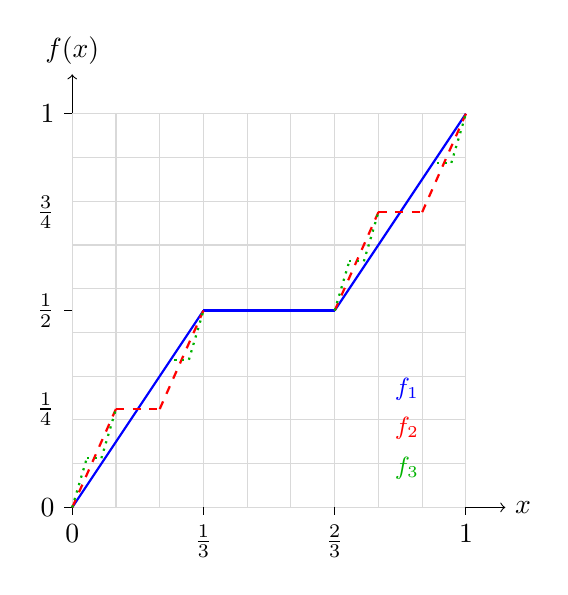
\begin{tikzpicture}[scale=5]
    % Axes
    \draw[->] (0,0) -- (1.1,0) node[right] {$x$};
    \draw[->] (0,0) -- (0,1.1) node[above] {$f(x)$};
    
    % Grid lines
    \draw[gray!30] (0,0) grid[step=1/9] (1,1);
    
    % Tick marks and labels on x-axis
    \foreach \x in {0, 1/3, 2/3, 1} {
        \draw (\x,0) -- (\x,-0.02);
    }
    \node[below] at (0,-0.02) {$0$};
    \node[below] at (1/3,-0.02) {$\frac{1}{3}$};
    \node[below] at (2/3,-0.02) {$\frac{2}{3}$};
    \node[below] at (1,-0.02) {$1$};
    
    % Tick marks and labels on y-axis
    \foreach \y in {0, 1/2, 1} {
        \draw (0,\y) -- (-0.02,\y);
    }
    \node[left] at (-0.02,0) {$0$};
    \node[left] at (-0.02,1/4) {$\frac{1}{4}$};
    \node[left] at (-0.02,1/2) {$\frac{1}{2}$};
    \node[left] at (-0.02,3/4) {$\frac{3}{4}$};
    \node[left] at (-0.02,1) {$1$};
    
    % Cantor function approximation (first few iterations)
    % Level 0: [0,1] -> [0,1]
    % Level 1: constant on (1/3, 2/3)
    \draw[thick, blue] (0,0) -- (1/3,1/2);
    \draw[thick, blue] (1/3,1/2) -- (2/3,1/2);
    \draw[thick, blue] (2/3,1/2) -- (1,1);
    
    % Level 2: constant on (1/9, 2/9) and (7/9, 8/9)
    \draw[thick, red, dashed] (0,0) -- (1/9,1/4);
    \draw[thick, red, dashed] (1/9,1/4) -- (2/9,1/4);
    \draw[thick, red, dashed] (2/9,1/4) -- (1/3,1/2);
    \draw[thick, red, dashed] (2/3,1/2) -- (7/9,3/4);
    \draw[thick, red, dashed] (7/9,3/4) -- (8/9,3/4);
    \draw[thick, red, dashed] (8/9,3/4) -- (1,1);
    
    % Level 3: even finer steps (showing the staircase nature)
    \draw[thick, green!70!black, dotted] (0,0) -- (1/27,1/8);
    \draw[thick, green!70!black, dotted] (1/27,1/8) -- (2/27,1/8);
    \draw[thick, green!70!black, dotted] (2/27,1/8) -- (1/9,1/4);
    \draw[thick, green!70!black, dotted] (7/27,3/8) -- (8/27,3/8);
    \draw[thick, green!70!black, dotted] (8/27,3/8) -- (1/3,1/2);
    
    % Additional fine structure
    \draw[thick, green!70!black, dotted] (2/3,1/2) -- (19/27,5/8);
    \draw[thick, green!70!black, dotted] (19/27,5/8) -- (20/27,5/8);
    \draw[thick, green!70!black, dotted] (20/27,5/8) -- (7/9,3/4);
    \draw[thick, green!70!black, dotted] (25/27,7/8) -- (26/27,7/8);
    \draw[thick, green!70!black, dotted] (26/27,7/8) -- (1,1);
    
    % % Endpoint dots
    % \fill[blue] (0,0) circle (0.8pt);
    % \fill[blue] (1/3,1/2) circle (0.8pt);
    % \fill[blue] (2/3,1/2) circle (0.8pt);
    % \fill[blue] (1,1) circle (0.8pt);
    
    % Legend
    \node[blue] at (0.85,0.3) {\small $f_1$};
    \node[red] at (0.85,0.2) {\small $f_2$};
    \node[green!70!black] at (0.85,0.1) {\small $f_3$};

    % Title
    % \node at (0.5,1.05) {\textbf{Cantor Function (Devil's Staircase)}};
\end{tikzpicture}
% \caption{The Cantor function showing its characteristic "devil's staircase" appearance. The function is constant on each removed interval from the Cantor set construction and increases only on the Cantor set itself.}
\label{fig:cantor_function}
\end{figure}

\begin{remark}
    The Cantor function has several remarkable properties:
    \begin{enumerate}
        \item It is continuous and non-decreasing on $[0,1]$.
        \item It maps $[0,1]$ onto $[0,1]$ surjectively.
        \item Its derivative is zero almost everywhere (on the complement of the Cantor set).
        \item It increases only on the Cantor set, which has measure zero.
        \item It is an example of a singular function: continuous but not absolutely continuous.
    \end{enumerate}
\end{remark}


\chapter{Causal Inference}
Rubin (1975\cite{rubin1975bayesian}) and Holland (1986\cite{holland1986statistics}) made up the aphorism\cite{ding2023causalinference}:
\begin{quote}
  \textit{``No causation without manipulation''}
\end{quote}
Not everybody agrees with this point of view.

In our lectuere, we'll define causal effects using the potential outcomes framework
(Neyman, 1923\cite{neyman1923experiment}; Rubin, 1974\cite{rubin1974estimating}).


\section{Potential Outcomes Framework}

In this framework, an experiment, or at least a thought experiment, 
has a treatment, and we are interested in its effect on an outcome 
or multiple outcomes. Sometimes, the treatment is also called an
intervention or a manipulation.

Firstly, we consider an experiment with $n$ units indexed by $i=1, 2, \cdots, n$.
We focus on a treatment with two levels:
\begin{gather*}
  d_i = \left\{\begin{matrix}
    0 & \text{control}\\
    1 & \text{treatment}
  \end{matrix} \right.
\end{gather*}

We seek to identify the causal effect of treatment $d_i$ on some outcome $y_i$.
For each $i$, the outcome od interest $y_i$ has two versions:
\begin{gather*}
  y_i = \left\{\begin{matrix}
    y_{0i} & d_i=0\\
    y_{1i} & d_i=1
  \end{matrix} \right.
\end{gather*}
This notation emphasizes that $y_{di}$ is the realization of the outcome $y_i$ that would materialize if unit $i$
received treatment $d_i = d$.

Neyman (1923\cite{neyman1923experiment}) first used this notation. It seems intuitive but has some hidden
assumptions. Rubin (1980\cite{rubin1980comment}) made the following clarifications on the hidden assumptions.
\begin{assumption}[No interference]\label{assumption:no_interference}
  \

  Unit $i$'s potential outcomes do not depend on other units' treatments. 
  This is sometimes called the no-interference assumption.
\end{assumption}
\begin{assumption}[Consistency]\label{assumption:consistency}
  \

  There are no other versions of the treatment. 
  Equivalently, we require that the treatment levels be well-defined, 
  or have no ambiguity at least for the outcome of interest. 
  This is sometimes called the consistency assumption.
\end{assumption}

The causal effect of the treatment on the $i$-th unit is then defined as:
\begin{gather*}
  \Delta_i = y_{1i} - y_{0i} 
\end{gather*}
These potential outcomes are constants at the level of unit $i$.

\begin{remark}[Problem of causal inference]
  \

  The fundamental problem in causal inference is that only one treatment can be assigned to a given individual, 
  and so only one of $y_{0i}$ and $y_{1i}$ can be observed. Thus $\Delta_i$ can never be observed.
\end{remark}

\begin{definition}[Stable Unit Treatment Value Assumption (SUTVA)]
\label{def:sutva}
  \

  Rubin (1980\cite{rubin1980comment}) called the Assumptions \ref{assumption:no_interference} and \ref{assumption:consistency} above together 
  the \textit{Stable Unit Treatment Value Assumption (SUTVA).}
\end{definition}
The observed outcome of unit $i$ is a function of the potential
outcomes and the treatment indicator, we can write:
\begin{gather*}
  y_i = d_i y_{1i} + (1 - d_i) y_{0i}
\end{gather*}
In principle, by virtue of being (discrete) RVs, both $d_i$ and $y_i$ each have a distribution function,
which, together with their possible realizations, defines various moments.
However, their unconditional probabilities and moments at the level of unit $i$ is not of interest.
Only the conditional probabilities of $y_i$ given $d_i$ is of interest.

\begin{remark}[Rubin (2005\cite{rubin2005causal})]
  \

  Under SUTVA, Rubin (2005) called the $n \times 2$ matrix of potential outcomes the Science Table:
  $$\begin{array}{ccc}
  \hline
  i & y_{1i}  & y_{0i}  \\
  \hline
  1 & y_{11}  & y_{01}  \\
  2 & y_{12}  & y_{02}  \\
  \vdots & \vdots & \vdots \\
  n & y_{1n}  & y_{0n} \\
  \hline
  \end{array}$$
  Due to the fundamental contributions of Neyman and Rubin to statistical causal inference, the potential outcomes framework is sometimes referred to as the Neyman Model, 
  the Neyman-Rubin Model, or the Rubin Causal Model.
  Causal effects are functions of the Science Table. Inferring individual causal effects
  $$\tau_i = y_{1i}  - y_{0i} , \quad (i=1,\ldots,n)$$
  is fundamentally challenging because we can only observe either $y_{1i} $ or $y_{0i}$,
  for each unit $i$, that is, we can observe only half of the Science Table.
\end{remark}

SUTVA(\ref{def:sutva}) ensures that the individual treatment effect is well defined.

Now, although $\Delta_i$ itself is unobservable, we can (perhaps remarkably) 
use randomized experiments to learn certain properties of it. The expectations
$\mathbb{E}[y_{0i}]$ and $\mathbb{E}[y_{1i}]$ denote the average potential outcomes across unit $i$ in population.

In particular, large randomized experiments let us recover the \textbf{Average
Treatment Effect (ATE)}:
\begin{gather*}
  \text{ATE} = \mathbb{E}[y_{1i} - y_{0i}] = \mathbb{E}[y_{1i}] - \mathbb{E}[y_{0i}]
\end{gather*}

For a population, we can define the treatment conditional expectations:
\[\mathbb{E}[y_i | d_i=1], \mathbb{E}[y_{0i} | d_i=1 ], \mathbb{E}[y_{1i} | d_i=1 ] = \mathbb{E}[y_i | d_i=1]\]
that denote the averages of the outcome $y_i$.

Analogously, we can define the control conditional expectations:
\[\mathbb{E}[y_i | d_i=0], \mathbb{E}[y_{0i} | d_i=0 ] = \mathbb{E}[y_i | d_i=0], \mathbb{E}[y_{1i} | d_i=0 ]\]
for the non-treated subpopulation.

Similar to ATE, we candefine the Average Treatment Effect for the Treatment-Group (ATT) and the Average
Treatment Effect for the Control-Group (ATC) as distinct objects:
\begin{align*}
  \text{ATT} &= \mathbb{E}[y_{1i}- y_{0i} | d_i=1]\\
  \text{ATC} &= \mathbb{E}[y_{1i}- y_{0i} | d_i=0]
\end{align*}
\[\mathbb{E}[z] = \mathbb{E}[z|d=1] \mathbb{P}[d=1] + \mathbb{E}[z|d=0] \mathbb{P}[d=0] = \mathbb{E}[\mathbb{E}[z|d]].\]

\subsection{Identification of Causal Effects}

Now, suppose we observe treatments and outcomes over a random sample $n$ from the overall population, $\{d_i, y_i\}_{i=1}^n = \{d_i, y_{d_{i}i}\}_{i=1}^n$, 
as either $y_I = y_{0i} $, or $y_i = y_{1i}$. 

Let $n_{w} = \vert \{ i: d_i = w \} \vert $ be the size of sets of units in our
sample who received and did not receive treatment, respectively.
This means that: while we observe a sample of size $n$ of $d_i$ and $y_i$ from the overall population,
we are observing a sample of size $n_0$ of realizations of $y_{0i}$ from the non-treated subpopulation 
and a sample of size $n_1$ of realizations of $y_{1i}$ from the treated subpopulation.

$N = \{i=1,2,\cdots, n\}$, $N_1 = \{i \in N: d_i = 1\} \leftarrow n_1 = \vert N_1 \vert $, $N_0 = \{i: d_i = 0\} \leftarrow n_0 = \vert N_0 \vert $.

Based on this data, we can use the analogy principle to consistently estimate 
the first term in the ATT formula and the second term in the ATC formula:
\begin{align*}
  \frac{1}{n_1} \sum_{i \in N_1} y_i &= \frac{1}{n_1} \sum_{i \in N_1} y_{1i} \overset{p}{\rightarrow} \mathbb{E}[y_{1i} | d_i=1] = \mathbb{E}[y_i | d_i=1]\\
  \frac{1}{n_0} \sum_{i \in N_0} y_i &= \frac{1}{n_0} \sum_{i \in N_0} y_{0i} \overset{p}{\rightarrow} \mathbb{E}[y_{0i} | d_i=0] = \mathbb{E}[y_i | d_i=0]
\end{align*}
Without further assumptions, we cannot identify the remaining terms. Firstly, we cannot observe $\mathbb{E}[y_{0i} | d_i=1]$ and $\mathbb{E}[y_{1i} | d_i=0 ]$
because we do not observe $y_{0i}$ for treated units, and we do not observe $y_{1i}$ for non-treated units.
Secondly, we can not observe $\mathbb{E}[y_{1i}]$ and $\mathbb{E}[y_{0i}]$ because both $N_1$ and $N_0$ are random samples from the overall population.
As a result, the ATE is in general not identified from our data!

We can define the  the difference-in-means estimator as:
\[\hat{\tau}_{DM} = \frac{1}{n_1} \sum_{i \in N_1} y_i - \frac{1}{n_0} \sum_{i \in N_0} y_i \overset{p}{\rightarrow} \mathbb{E}[y_{1i} | d_i = 1] - \mathbb{E}[y_{0i} | d_i = 0] = \text{ATE} = \text{ATT} = \text{ATC}.\]


We define the difference of treated and non-treated as: \textit{Naive Difference}.
\begin{align*}
  \text{ND} &= \mathbb{E}[y_{1i} | d_i = 1] - \mathbb{E}[y_{0i} | d_i = 0]\\
  &= \mathbb{E}[y_{1i} | d_i = 1] - \mathbb{E}[y_{0i} | d_i = 1] + \mathbb{E}[y_{0i} | d_i =1] - \mathbb{E}[y_{0i} | d_i = 0] \\
  &= ATT + \mathbb{E}[y_{0i} | d_i = 1] - \mathbb{E}[y_{0i} | d_i = 0]
\end{align*}

For LRM, $y_i = \beta_0 + \beta_1 d_i + u_i$,
\begin{align*}
  \text{ND} &= \mathbb{E}[y_i | d_i = 1] - \mathbb{E}[y_i | d_i = 0]\\
  &= \mathbb{E}[\beta_0 + \beta_1 + u_i | d_i = 1] - \mathbb{E}[\beta_0 + u_i | d_i = 0]\\
  &= \beta_1 + \mathbb{E}[u_i | d_i = 1] - \mathbb{E}[u_i | d_i = 0]  
\end{align*}



\[
\{Y_d\} \perp\!\!\!\perp D \mid X \implies \{Y_d\} \perp\!\!\!\perp D \mid \pi(X), \quad D \perp\!\!\!\perp X \mid \pi(X)
\]
\chapter{Panel Data Analysis}
Economists traditionally use the term \textbf{panel data} to refer to data structures consisting of observa-
tions on individuals for multiple time periods. 
There are several distinct advantages of panel data relative to cross-section data:
\begin{enumerate}
  \item Possibility of controlling for unobserved time-invariant endogeneity without the use of instrumental variables
  \item Possibility of allowing for broader forms of heterogeneity
  \item Modeling dynamic relationships and effects
\end{enumerate} 

It's typical to index observations by both the individual $i$ and the time period, $t$,
thus $y_{it} $ denotes a variable for indivual $i$ in time $t$, where $n=1, \cdots, N$, $t=1, \cdots, T.$

\begin{definition}[Balanced and Unbalanced Panel Data\cite{hansen2022econometrics}]
  \

  When observations are available on all individuals for the same time periods we say that the panel is \textbf{balanced}. 
  In this case there are an equal number $T$ of observations for each individual and the total number of observations is $n = NT$.

  When different time periods are available for the individuals in the sample we say that the panel is \textbf{unbalanced}. 
  This is the most common type of panel data set. 
  It does not pose a problem for applications but does make the notation cumbersome and also complicates computer programming.
\end{definition}

\section{Incidental Parameters Problem}

\subsection{Pooled OLS Estimation}\label{sec:POLS}

Suppose we are estimating the following panel data regression:
\begin{align*}
  y_{it} &= \alpha +x_{it}^{\prime} \beta +u_{it}, \quad \mathbb{E}[u_{it} x_{it}] = 0, \quad \mathbb{V}[u_{it} | x_{it}] = \sigma^2
\end{align*}

Omitting the distinction between intercept and slope, we can write the model as:
\begin{gather*}
  y_{it} = \tilde{x}_{it}^{\prime} \tilde{\beta} + u_{it} \\
  \tilde{x}_{it} = \begin{bmatrix}
    1 \\
    x_{it}
  \end{bmatrix}, \quad
  \tilde{\beta} = \begin{bmatrix}
    \alpha \\
    \beta
  \end{bmatrix}
\end{gather*}
where $i=1:n$, $T=1:t$.

Or, we can write the model as: 
\[ 
\underset{T\times 1}{y_i} = \underset{T \times K}{\tilde{X}_i} \underset{K \times 1}{\tilde{\beta}} + \underset{T \times 1}{u_i}
\]
Using OLS method to estimate $\tilde{\beta}$, we have:
\[
\underset{\tilde{\beta}}{\min} \sum_i \sum_t u_{it}^2 = \underset{\tilde{\beta}}{\min} \sum_i u_i^{\prime} u_i = \underset{\tilde{\beta}}{\min} (y_i - \tilde{X}_i \tilde{\beta})^{\prime} (y_i - \tilde{X}_i \tilde{\beta})
\]
The FOC of this equation is:
\begin{align*}
  \sum_i -\tilde{X}_i^{\prime} (y_i - \tilde{X}_i \tilde{\beta}) &= 0 \\
  \left(\sum_i \tilde{X}_i^{\prime} \tilde{X}_i \right) \tilde{\beta} &= \sum_i \tilde{X}_i^{\prime} y_i \\
  \hat{\tilde{\beta}}_{POLS} &= \left(\sum_i \tilde{X}_i^{\prime} \tilde{X}_i \right)^{-1} \sum_i \tilde{X}_i^{\prime} y_i \\
  &= \left(\sum_i \sum_t \tilde{x}_{it} \tilde{x}_{it}^{\prime} \right)^{-1} \left( \sum_i \sum_t \tilde{x}_{it} y_{it} \right) \\
  &= \tilde{\beta} + \left(\frac{1}{n} \sum_i \sum_t \tilde{x}_{it} \tilde{x}_{it}^{\prime} \right)^{-1} \left( \sum_i \sum_t \tilde{x}_{it} u_{it} \right) \\
  & \overset{p}{\rightarrow} \tilde{\beta} + \mathbb{E}\left[\sum_t \tilde{x}_{it} \tilde{x}_{it}^{\prime} \right] \mathbb{E}\left[\sum_t \tilde{x}_{it} u_{it} \right] \\
  &= \tilde{\beta}
\end{align*}
Hence $\hat{\beta}_{OLS}$ is consistent provided that $x_{it}$ and $u_{it}$ are contemperaneously uncorrelated,
as $\mathbb{E}[x_{it} u_{it}] = 0, \forall t.$
The regressors are allowed to be correlated with the past, and future $u_{it}$.
This occurs when there's feedback loop by which $y_{i,t-1}$ affects $x_{it}$.

In this proof, we show that either $N \to \infty $ or $T \to  \infty $ is sufficient for consistency of $\hat{\beta}_{POLS}$.
However, most panel data applications have a large $n$ and small $T$ dimension, so standrad panel data
features $T$ fixed and $n \to \infty $.

\subsection{Asymptotic Normality}

From the analysis of consistency, we know that:
\[ 
\hat{\tilde{\beta}}_{POLS}  = \left(\sum_i \tilde{X}_i^{\prime} \tilde{X}_i \right)^{-1} \sum_i \tilde{X}_i^{\prime} y_i
\]
Hence:
\begin{align*}
    \sqrt{n} (\hat{\tilde{\beta}}_{POLS}  - \tilde{\beta}) &= \left(\frac{1}{n} \sum_i \tilde{X}_i^{\prime} \tilde{X}_i \right)^{-1} \left(\frac{1}{\sqrt{n} } \sum_i \tilde{X}_i^{\prime} u_i \right) \\
    & \overset{p}{\rightarrow}\mathbb{E}[\tilde{X}_i^{\prime} \tilde{X}_i]^{-1} \overset{d}{\rightarrow} \mathcal{N}\left(0, \mathbb{E}\left[\left(\tilde{X}_i^{\prime} u_i\right) \left(\tilde{X}_i^{\prime} u_i\right)^{\prime} \right] \right)\\
    & \overset{d}{\rightarrow} \mathcal{N} \left(0, \mathbb{E}\left[\tilde{X}_i^{\prime} \tilde{X}_i \right]^{-1} \mathbb{E}\left[\tilde{X}_i^{\prime} u_i u_i^{\prime} \tilde{X}_i \right] \mathbb{E}\left[\tilde{X}_i^{\prime} \tilde{X}_i \right] \right)
\end{align*}


The above model is homogeneous, which is unattractive, as the data generating process would 
differ across $i$, with some units having a higher level of the outcome variable $y_{it} $
than others, regardless of covariates $x_{it}$(with a higher intercept $\alpha$) or a stronger effect
of some covariates $x_{it, k} $ on $y_{it}$ than others.

At the other extreme, we assume the fully heterogenous estimation:
\[y_{it} = \alpha_i + x_{it}^{\prime} \beta + u_{it}, \quad \mathbb{E}[u_{it} x_{it}] = 0, \quad \mathbb{V}[u_{it} | x_{it}] = \sigma_i^2. \]

Under $T=1$, we run $y_i = \beta_0 + x_i^{\prime} \beta + v_i$, 
where $v_i = u_i + \underset{\tilde{\alpha}_i}{\underbrace{\alpha_i - \beta_0}}$
and $\mathbb{E}[v_i] = 0$.

Under $T>1$, we run:
\begin{align*}
    y_i &= x_i^{\prime} \beta  + \sum_{j=1}^{n} \alpha_j \mathbf{1}\{i=j\} + u_{it} \\
    &= \tilde{x}_{it}^{\prime} \tilde{\beta} + u_{it} \\
    \tilde{x}_{it} &= \begin{bmatrix}
      x_{it} \\
      \mathbf{1}\{i=1\} \\
      \mathbf{1}\{i=2\} \\
      \vdots \\
      \mathbf{1}\{i=n\}
    \end{bmatrix}, \quad
    \tilde{\beta} = \begin{bmatrix}
      \beta \\
      \alpha_1 \\
      \alpha_2 \\
      \vdots \\
      \alpha_n
    \end{bmatrix}
\end{align*}

In a similar way, we can write the regression as
\[y_{i}  = \tilde{X}_i \tilde{\beta}_i + u_i \]
with $\tilde{\beta}_i$ is specific for each $i$.
We have $n$ separate time series regressions, one for each unit $i$. 

Following the same analyzing process, we can get:
\[
\hat{\tilde{\beta}}_{i,OLS} = \Bigl( \sum_i \tilde{X}_i^{\prime} \tilde{X}_i \Bigr) \sum_i \tilde{X}_i^{\prime} y_i = \Bigl( \sum_t \tilde{x}_{it} \tilde{x}_{it}^{\prime} \Bigr)^{-1} \Bigl( \sum_t \tilde{x}_{it} y_{it} \Bigr),
\]
which obviously shows that $\hat{\tilde{\beta}}$ is consistent $\operatorname{\iff}$ $T \rightarrow\infty $.

\subsection{One-way error component model}\label{sec:one-way error component model}
With the fully homogeneous specification unattractive and the fully heterogeneous specifi-
cation infeasible, researchers usually go for a compromise and let intercepts (and error term
variances) be unit-specific.

\begin{definition}[One-way error component model]
  \begin{equation}
    y_{it}  = \alpha_i + x_{it}^{\prime} + u_{it}, \quad \mathbb{E}[u_{it} x_{it}] = 0, \quad \mathbb{V}[u_{it} | x_{it}] = \sigma^2, \label{eq: basic model}
  \end{equation}
where $\alpha_i$ is an individual-specific effect, and $u_{it}$ are idiosyncratic(i.i.d.) errors.
\end{definition}

In any case, the equation above makes clear that $\alpha_i $ contains all factors that affect $y_{it}$, that are
not included in $x_{it}$ and that are fixed over time (the time-varying factors are in $u_{it}$).

Suppose hte model is correctly specified, and we have a cross-sectional detaset available, i.e. $T=1$.
Then, we would estimate:
\[y_{it} = \beta_0 + x_{it}^{\prime} + v_i, \text{ for} t=1,\]
where $v_i = \alpha_i + u_{it} -\beta_0.$

If the unobserved heterogeneity $\alpha_i$ is correlated with the covariate $x_{it} $,
our standard OLS estimator is biased and inconsistent.

If we have a panel dataset, i.e. $T>1$, we can write the above model into a regression of $k+n$ regressors:
\[
y_{it} = x_{it}^{\prime} \beta + \sum_{j=1}^{n}\mathbf{1}\{i=j\} \alpha_j + u_{it} = x_{it}^{*^{\prime}} \beta^* + u_{it},
\]
where $x_{it}^* = \Bigl( x_{it}^{\prime}, \mathbf{1}\{i=1\}, \cdots, \mathbf{1}\{i=n\} \Bigr)^{\prime} $,
and $\beta^* = \Bigl( \beta^{\prime}, \alpha_1, \cdots, \alpha_n \Bigr)^{\prime}.$

This leads to the pooled OLS estimator for $\beta^*$:
\[
\hat{\beta}^* = \Bigl( \sum_i \sum_t x_{it}^* x_{it}^{*^{\prime}} \Bigr) \sum_i \sum_t x_{it}^* y_{it}. 
\]

However, the estimator suffers from the so-called \textbf{IPP problem}, 
as the number of parameters increase with $n \rightarrow\infty $, 
the limit of $\frac{1}{n} \sum_i x_{it}^* x_{it}^{*^{\prime}}$ is not well-defined
and as a result, we can't establish consistency of $\hat{\beta}_{OLS}.$
\section{Random Effects}

As with pooled OLS, a random effects analysis puts $\alpha_i$ into the error term.
In fact, random effects analysis imposes more assumptions than those needed for pooled OLS:
\textbf{strict exogeneity} in addition to orthogonality between $\alpha_i$ and $x_{it}$. 

\subsection{Basic Assumptions and POLS}

Stating the assumption in terms of conditional means, we have:
\begin{assumption}[Random Effect]\label{assumption:RE}
    \

    \begin{enumerate}
        \item[(a)] $\mathbb{E}[u_{it} | X_i, \alpha_i] = 0, \forall t.$
        \item[(b)] $\mathbb{E}[\alpha_i | X_i] = \mathbb{E}[\alpha_i] = 0.$
    \end{enumerate}
    where $X_i = (x_{i1}, \cdots, x_{iT})$.
\end{assumption}
Assumption \ref{assumption:RE}(a) is the strict exogeneity condition and Assumption \ref{assumption:RE}(b) is is how we will state the orthogonality.

\begin{remark}[Why Strict Ecogeneity?\cite{wooldridge2010econometric}]
    \

    Why do we maintain Assumption \ref{assumption:RE}(a) when it is more restrictive than needed for
    a pooled OLS analysis? Because the random e¤ects approach exploits the serial correlation in
    the composite error, $v_{it} = \alpha_i + u_{it}$, in a generalized least squares (GLS) framework. In
    order to ensure that feasible GLS is consistent, we need some form of strict exoge-
    neity between the explanatory variables and the composite error.

    Under this assumption, we can write:
    \begin{align*}
        & y_{it} = x_{it}^{\prime} \beta + v_{it} \\
        & \mathbb{E}[v_{it} | X_i] = 0, t=1, \cdots, T
    \end{align*}
    The conditions shows that our model satisfies the GLS assumption, which confirms that
    we can apply GLS methods that account for the particular error structure $v_{it} = \alpha_i + u_{it}.$
\end{remark}


By defining $v_{it} = u_{it} + \alpha_i - \beta_0$, we can transform the random effect model to the following:
\begin{align*}
    y_{it} &= \alpha_i + x_{it}^{\prime} \beta + u_{it} \\
    &= \underset{\tilde{x}_{it}^{\prime}}{\underbrace{\beta_0 + x_{it}^{\prime}\beta}} + \underset{\equiv v_{it}}{\underbrace{u_{it} + \alpha_i - \beta_0}}
\end{align*}
Defining again $\tilde{x}_{it} = (1, x_{it}^{\prime})^{\prime}$, $\tilde{\beta} = (\beta_0, \beta^{\prime})^{\prime}$, we can rewrite the model as:
\begin{align*}
    y_{it} &= \tilde{x}_{it}^{\prime} \beta + v_{it} \Leftrightarrow y_i = \tilde{X}_i^{\prime} \tilde{\beta} + v_i \\
    \rightarrow \hat{\tilde{\beta}} &= \left(\sum_i \tilde{X}_i^{\prime} \tilde{X}_i \right)^{-1} \sum_i \tilde{X}_i^{\prime} y_i
\end{align*}

With this intercept $beta_0$, $\mathbb{E}[v_i] = 0$ is guaranteed to hold.
Define $\tilde{\alpha}_i = \alpha_i - \beta_0$ as the mean-zero unit-specific heterogenety so that $v_i = u_i + \tilde{\alpha}_i.$


\begin{note}[POLS]
    \

    Homogenous spec: $y_{it} = \alpha  + x_{it}^{\prime} \beta + u_{it} = \tilde{x}_{it}^{\prime} \tilde{\beta} + v_{it}.$
    $\hat{\tilde{\beta}}$ is consistent if $\mathbb{E}[v_{it} x_{it}]=0, \forall t.$
\end{note}
Using pooled OLS to estimate $\hat{\tilde{\beta}}$,
\begin{align*}
    \hat{\tilde{\beta}}_{RE-OLS/POLS} &= \left(\frac{1}{n} \sum_i \tilde{X}_i^{\prime} \tilde{X}_i \right)^{-1} \frac{1}{n} \sum_i \tilde{X}_i^{\prime} y_i \\
    &= \tilde{\beta} + \left(\frac{1}{n} \sum_i \tilde{X}_i^{\prime} \tilde{X}_i \right)^{-1} \frac{1}{n} \sum_i \tilde{X}_i^{\prime} v_i \\
    &\overset{p}{\rightarrow} \tilde{\beta} + \mathbb{E}[\tilde{X}_i^{\prime} \tilde{X}_i]^{-1} \mathbb{E}[\tilde{X}_i^{\prime} v_i] \\
    \text{where} \quad \mathbb{E}[\tilde{X}_i^{\prime} v_i] &= \mathbb{E}\left[\sum_t \tilde{x}_{it}^{\prime} v_{it} \right] \\
    &= \sum_t \mathbb{E}\left[\tilde{x}_{it}^{\prime} v_{it}  \right] \\
    &= \sum_t \mathbb{E}\left[\tilde{x}_{it}(u_{it} + \alpha_i - \beta_0)\right]
\end{align*}
Here, the error term $v_i$ is not equal to the original error term $u_{it}$.
\begin{note}
    \

    Under the random effect, you have to use the heteroskedasticity-robust methods.
    Because even if we assume $u_{it}$ to be homoskedastic, $v_{it}$ is not,
    as it includes also the unit-specific heterogeneity $\alpha_i$.
\end{note}

\subsection{From POLS to GLS}

So, to obtain consistency, we need to assume that:
\begin{itemize}
    \item $\mathbb{E}[u_{it} | \tilde{x}_{it}, \tilde{\alpha}_i] = 0, \forall t$.
    \item $\mathbb{E}[\tilde{\alpha_i} | \tilde{x}_{it}] = 0, \forall t$.
\end{itemize}
And, we are also obliged to use HAC-robust standard error because:
\[\Omega \equiv \mathbb{E}[v_i v_i^{\prime} | \tilde{X}_i] = \mathbb{E}[(\alpha_i \mathbf{1}_i + u_i)(\tilde{\alpha}_i \mathbf{1}_i + u_i)^{\prime} | \tilde{X}_i] = \mathbb{E}[\tilde{\alpha}_i^2 \mathbf{1}_i \mathbf{1}_i^{\prime} | \tilde{X}_i] + \mathbb{E}[u_i u_i'| \tilde{X}_i] \]
is not diagonal.

\begin{assumption}[Random Effect]\label{assumption:RE2}
    \

    $\rank \mathbb{E}\left[X_i^{\prime} \Omega^{-1} X_i \right] = K$
\end{assumption}
We know that both GLS and feasible GLS estimator would be consistent under Asusmption \ref{assumption:RE} and \ref{assumption:RE2}.
A general FGLS analysis, using an unrestricted variance estimator $\Omega$,
is consistent and asymptotically normal as $N \to \infty.$

But, we won't exploit the unobserved effects structure $v_{it}.$
A standard random e¤ects analysis adds assumptions on the idiosyncratic errors that
give $\Omega$ a special form. The first assumption is that the idiosyncratic errors
$u_{it}$ have a constant unconditional variance across $t$:
\begin{assumption}[RE-Homoskedasticity]\label{assumption:RE-homoskedasticity}
    \

    $\mathbb{E}[u_{it}^2] = \sigma_u^2, \forall t$
\end{assumption}
The second assumption is that the idiosyncratic errors are serially uncorrelated:
\begin{assumption}[RE-Serial Uncorrelated]\label{assumption:RE-serial_uncorrelated}
    \

    $\mathbb{E}[u_{it} u_{is}] = 0, \forall t \neq s$
\end{assumption}
Under these two assumptions, we can derive the variances and covariances of the
elements of $v_i$.
Given the error structure the natural estimator for $\beta$ is GLS. The GLS eimator for $\beta$ is:
\begin{gather*}
    \hat{\tilde{\beta}}_{RE-GLS} = \left( \sum_i \tilde{X}_i^{\prime} \Omega^{-1} \tilde{X}_i \right)^{-1} \sum_i \tilde{X}_i^{\prime} \Omega^{-1} y_i
\end{gather*}
where $\Omega ^{-\frac{1}{2}} y_i = \Omega ^{-\frac{1}{2}} \tilde{X}_i^{\prime} \tilde{\beta} + \Omega^{-\frac{1}{2}}v_i.$
\begin{align*}
    \Omega &= \mathbb{E}[v_i v_i^{\prime} | \tilde{X}_i] = \mathbb{E}\left[ \begin{bmatrix}
        v_{i1} \\
        v_{i2} \\
        \vdots \\
        v_{iT}
    \end{bmatrix} \begin{bmatrix}
        v_{i1} & v_{i2} & \cdots & v_{iT}
    \end{bmatrix} | \tilde{X}_i \right]\\
    &= \mathbb{E}\begin{bmatrix}
        \mathbb{E}[v_{i1}^2 | \tilde{X}_i] & \mathbb{E}[v_{i1}v_{i2} | \tilde{X}_i] & \cdots & \mathbb{E}[v_{i1}v_{iT} | \tilde{X}_i] \\
        \mathbb{E}[v_{i2}v_{i1} | \tilde{X}_i] & \mathbb{E}[v_{i2}^2 | \tilde{X}_i] & \cdots & \mathbb{E}[v_{i2}v_{iT} | \tilde{X}_i] \\
        \vdots & \vdots & \ddots & \vdots \\
        \mathbb{E}[v_{iT}v_{i1} | \tilde{X}_i] & \mathbb{E}[v_{iT}v_{i2} | \tilde{X}_i] & \cdots & \mathbb{E}[v_{iT}^2 | \tilde{X}_i]
    \end{bmatrix} \\
    &= \begin{bmatrix}
        \mathbb{E}\left[\alpha_i^2 | \tilde{X}_i \right] + \mathbb{E}[u_{i1}^2 | \tilde{X}_i] & \mathbb{E}\left[\alpha_i^2 | \tilde{X}_i \right] + \mathbb{E}[u_{i1}u_{i2} | \tilde{X}_i] & \cdots & \mathbb{E}\left[\alpha_i^2 | \tilde{X}_i \right] + \mathbb{E}[u_{i1}u_{iT} | \tilde{X}_i] \\
        \mathbb{E}\left[\alpha_i^2 | \tilde{X}_i \right] + \mathbb{E}[u_{i2}u_{i1} | \tilde{X}_i] & \mathbb{E}\left[\alpha_i^2 | \tilde{X}_i \right] + \mathbb{E}[u_{i2}^2 | \tilde{X}_i] & \cdots & \mathbb{E}\left[\alpha_i^2 | \tilde{X}_i \right] + \mathbb{E}[u_{i2}u_{iT} | \tilde{X}_i] \\
        \vdots & \vdots & \ddots & \vdots \\
        \mathbb{E}\left[\alpha_i^2 | \tilde{X}_i \right] + \mathbb{E}[u_{iT}u_{i1} | \tilde{X}_i] & \mathbb{E}\left[\alpha_i^2 | \tilde{X}_i \right] + \mathbb{E}[u_{iT}u_{i2} | \tilde{X}_i] & \cdots & \mathbb{E}\left[\alpha_i^2 | \tilde{X}_i \right] + \mathbb{E}[u_{iT}^2 | \tilde{X}_i]
    \end{bmatrix}\\
    &= \begin{bmatrix}
        \sigma_u^2 + \sigma_{\alpha}^2 & \sigma_{\alpha}^2 & \cdots & \sigma_{\alpha}^2 \\
        \sigma_{\alpha}^2 & \sigma_u^2 + \sigma_{\alpha}^2 & \cdots & \sigma_{\alpha}^2 \\
        \vdots & \vdots & \ddots & \vdots \\
        \sigma_{\alpha}^2 & \sigma_{\alpha}^2 & \cdots & \sigma_u^2 + \sigma_{\alpha}^2
    \end{bmatrix} \\
    &= \sigma_{\alpha}^2 \mathbf{1}_i \mathbf{1}_i^{\prime} + \sigma_u^2 I \\
    \text{beacuse } &\mathbb{V}[\tilde{\alpha}_i|\tilde{X}_i] = \sigma_{\alpha_i}^2 = \sigma_{\alpha}^2 \\
    &\mathbb{V}[u_{it} | \tilde{X}_i] = \sigma_u^2, \forall i.
\end{align*}
where $I$ is an identity matrix of dimention $T_i$.
Under the assumption $\mathbb{E}[u_{it} x_{is}] = 0$, we now describe some statistical properties of $\hat{\tilde{\beta}}_{RE-GLS}.$

\subsubsection{RE Consistency}
\begin{align*}
    \hat{\tilde{\beta}}_{RE-GLS} - \tilde{\beta} &= \Bigl( \sum_i \tilde{X}_i^{\prime} \Omega^{-1} \tilde{X}_i \Bigr)^{-1} \Bigl( \sum_i \tilde{X}_i^{\prime} \Omega^{-1} v_i \Bigr) \\
    & \rightarrow \mathbb{E}\Bigl[ \sum_i \tilde{X}_i^{\prime} \Omega^{-1} \tilde{X}_i \Bigr] \mathbb{E}\Bigl[ \sum_i \tilde{X}_i^{\prime} \Omega^{-1} v_i \Bigr] \\
    \text{where } \mathbb{E}\Bigl[ \sum_i \tilde{X}_i^{\prime} \Omega^{-1} v_i \Bigr] &= \sum_i \mathbb{E}\Bigl[ \tilde{X}_i^{\prime} \Omega^{-1} v_i \Bigr] \\
    &= \sum_i \tilde{X}_i^{\prime} \Omega^{-1} \mathbb{E}[v_i | \tilde{X}_i] \\
    &= \sum_i \tilde{X}_i^{\prime} \Omega^{-1} \mathbb{E}[u_i + \tilde{\alpha}_i | \tilde{X}_i] \\
    &=0
\end{align*}
Thus, $\hat{\tilde{\beta}}_{RE-GLS} $ is conditionally unbiased for $\tilde{\beta}$.
The conditional variance of $\hat{\tilde{\beta}}_{RE-GLS}$ is:
\begin{align*}
    \mathbb{V}\Bigl[\hat{\tilde{\beta}}_{RE-GLS}\Bigr] = \Bigl( \sum_i \tilde{X}_i^{\prime} \Omega^{-1} \tilde{X}_i \Bigr)^{-1} \sigma_{u}^2
\end{align*}

\subsubsection{RE Asymptotic Distribution}
The asymptotic variance of $\hat{\tilde{\beta}}_{RE-GLS}$ is:
\begin{align*}
    &\sqrt{n} \left( \hat{\tilde{\beta}}_{RE-GLS} - \tilde{\beta} \right) \overset{d}{\rightarrow} \mathcal{N}\left(0, V \right) \\
    \text{where } V_{GLS}  &= \mathbb{E}\left[\tilde{X}_i^{\prime} \Omega^{-1} \tilde{X}_i \right]^{-1} \mathbb{E}\left[\tilde{X}_i^{\prime} \Omega^{-1} v_i v_i^{\prime} \Omega^{-1} \tilde{X}_i \right] \mathbb{E}\left[\tilde{X}_i^{\prime} \Omega^{-1} \tilde{X}_i \right] \\
    &= \mathbb{E}\left[\tilde{X}_i^{\prime} \Omega^{-1} \tilde{X}_i \right]^{-1} \underset{\equiv \Omega}{\underbrace{\mathbb{E}[v_i v_i^{\prime} | \tilde{X}_i]}}
\end{align*}
Because we do not know $\Omega$, the RE-GLS estimator is infeasible. 

If indeed we have:
\begin{align*}
    \Omega &= \mathbb{E}[v_i v_i^{\prime}  | \tilde{X}_i] \\
    &= \mathbb{E}[(\alpha_i \mathbf{1}_i + u_i)(\alpha_i \mathbf{1}_i  + u_i)^{\prime}  | \tilde{X}_i] \\
    &= \mathbb{E}[\alpha_i^2] \mathbf{1}_i \mathbf{1}_i^{\prime} + \mathbb{E}[u_i u_i^{\prime} | \tilde{X}_i]
\end{align*}
which implies homoskedasticity.

A feasible version replaces $\Omega$ with an estimator $\hat{\Omega}_i$.
Assuming homoskedasticity of the original errors:
\begin{align*}
    \mathbb{E}[u_i u_i^{\prime}  | \tilde{X}_i, \tilde{\alpha}_i] &= \sigma_u^2 I_T \\
    \mathbb{E}[\tilde{\alpha}_i^2 | \tilde{x}_i] &= \sigma_{\alpha}^2
\end{align*}
We obtain: $\hat{\Omega} = \hat{\sigma}_{\alpha}^2 \mathbf{1}_i \mathbf{1}_i^{\prime} + \hat{\sigma}_u^2 I_T$, 
a $T \times T$ matrix that we assume to be positive definite.
In a panel data context, the FGLS estimator that uses this variance matrix is what is known as the \textbf{random effects estimator}.

Hence, the motivation for using GLS is different than under a cross-sectional regression with heteroskedasticity.
We use GLS because of the autocorrelation in $v_{it}$ induced by the presence of time variant $\alpha_i$.

\subsection{Comparing POLS and GLS}

Now, let's compare the $\hat{\beta}_{RE-GLS}$ with the pooled estimator $\hat{\beta}_{POLS}$.

Under the assumptions of the random effects model, POLS estimator is also unbiased for $\beta$ and has conditional variance:
\begin{gather*}
    V_{POLS} = \Bigl(\sum_{i} X_i^{\prime} X_i \Bigr)^{-1} \Bigl( X_i^{\prime} \Omega_i X_i \Bigr)^{-1} \Bigl( X_i^{\prime} X_i \Bigr)^{-1} 
\end{gather*}
Using the algebra of the Gauss-Markov Theorem we deduce that:
\[V_{RE-GLS} \leq V_{POLS} \]
and thus the random effects estimator $\hat{\beta}_{RE-GLS}$ is more efficient than $\hat{\beta}_{POLS} $ under the strict exogeneity assumption \ref{assumption:RE}.
The two variance matrices are identical when there is no individual-specific effect $\sigma_{\alpha}^2 = 0$ for then $V_{RE-GLS} = V_{POLS} = \left(X^{\prime} X\right)^{-1} \sigma_u^2.$

Under the asusmption that the random effects model is a useful approximation but not literally true, 
we may use the cluster-robust covariance matrix estimator such as:
\begin{gather*}
    \hat{V}_{RE-GLS} = \Bigl(\sum_{i} X_i^{\prime} \Omega_i X_i\Bigr)^{-1} \Bigl( \sum_{i} X_i^{\prime} \Omega_i \hat{v}_i \hat{v}_i^{\prime} \Omega_i^{\prime} X_i \Bigr)^{-1} \Bigl( \sum_{i} X_i^{\prime} \Omega_i X_i \Bigr)^{-1} 
\end{gather*}
where $\hat{v}_i = y_i - X_i \hat{\beta}_{RE-GLS}$, This may be re-scaled by a degree of freedom adjustment if desired.

\section{Fixed Effects}
In the econometrics literature if the stochastic structure of $\alpha_i$ is treated as unknown
and possibly correlated with $x_{it}$, then $\alpha_i$ is called a \textbf{fixed effect}.

Correlation between $\alpha_i$ and $x_{it}$ will cause both pooled and random effect estimators ro be biased.

We transform equation to get rid of $\alpha_i$: $y_{it} = \alpha_i + x_{it}^{\prime} \beta + u_{it}.$
This is due to the classic problems of omitted variables bias and endogeneity. 

The presence of the unstructured individual effect $\alpha_i$ means that it is not possible to identify $\beta$ under a simple projection assumption such as $\mathbb{E}[u_{it} x_{it}] = 0$.
It turns out that a sufficient condition for identification is the following.

\begin{definition}[Strictly exogeneity]\label{def:strictly_exogeneity}
    \

    A regressor $x_{it}$ is said to be strictly exogeneity if $\mathbb{E}[x_{it} u_{is}] = 0, \forall t, s = 1, \cdots, T$.
\end{definition}
Strict exogeneity is a strong projection condition,  meaning that is a $X_{is}, s \neq t$ is added into the regression model,
it would have a zero coefficient. Strict exogeneity is a projection analog of the \textbf{strict mean independence}\label{FE:SMI}:
\[\mathbb{E}[u_{it} | X_i] = 0\] 
which implies the strict exogeneity but not vice versa.

The strict exogeneity assumption \ref{def:strictly_exogeneity} is sufficient for identification and
asymptotic theory, we'll also use the strict mean independence assumption for finite sample analysis.

\begin{remark}[About strict exogeneity\cite{hansen2022econometrics}]
    \

    Strict ecogeneity(assumption \ref{def:strictly_exogeneity}) is typically inappropriate in dynamic models.
\end{remark}

\subsection{Within Transformation}

In previous steps, we showed that if $x_{it}$ and $\alpha_i$ are correlated, then pooled OLS and RE-GLS estimator would be biased and inconsistent.
If we leave the relationship between $\alpha_i$ and $x_{it}$ fully unstructured,
then the only way to consistently estimate the coefficient $\beta$ is by an estimator
which is invariant to $\alpha_i$.

The first fixed effects (FE) assumption is strict exogeneity of the explanatory variables conditional on $\alpha_i$:
\begin{assumption}[FE Strict Exogeneity]\label{assumption:FE-strictexogeneity}
    \

    $\mathbb{E}[u_{it} | X_i, \alpha_i] = 0, \forall t=1,\cdots, T$
\end{assumption}
This assumption is identical to the assumption \ref{assumption:RE}(a), we maintain strict exogeneity of $x_{it}, t=1, \cdots, T$
conditional on the unobserved effect.
The key difference is that \emph{we do not assume assumption \ref{assumption:RE}(b), which means that,
for FE analysis, $\mathbb{E}[\alpha_i | X_i]$ can be any function of $X_i$.}

By relaxing assumption \ref{assumption:RE}(b), we can conssitently estimate partial effects in the presence of time-consistent omitted variables
that can be arbitrarily related to unobserved variables $x_{it}$.
\emph{Therefore, FE analysis is more robust than RE analysis.}

But this robustness has a cost: we can not include any time-constant variables in $x_{it}$ without further assumptions.
The reason is simple: if $\alpha_i$ can be arbitrarily correlated with each element of $x_{it}$, 
then there's no way to distinguish the effect of time-constant observables from the time-constant unobservable $\alpha_i$.

The first transformation is the \textbf{within transformation}.
Define the mean of a variable for a given individual as
\begin{align*}
    \overline{y}_i &= \frac{1}{T} \sum_t y_{it} \\
    \overline{x}_i &= \frac{1}{T} \sum_t x_{it} \\
    \overline{u}_i &= \frac{1}{T} \sum_t u_{it}
\end{align*}
We call this the \textbf{individual-specific mean} since it is the mean of a given individual. \footnote{Some
authors call this the \textbf{time-average} or \textbf{time-mean} since it is the average over the time periods.}

Then, subtracting the individual-specific mean from the variable we obtain the deviations:
\begin{align*}
    (y_{it} - \overline{y}_i) &= (x_{it} - \overline{x}_i)^{\prime} \beta + (u_{it} -\overline{u}_i) + (\alpha_i - \alpha_i) \\
    \ddot{y}_{it} &= \ddot{x}_{it}^{\prime} \beta + \ddot{u}_{it} \\
    \ddot{y}_i &= \ddot{X}_i^{\prime} \beta + \ddot{u}_i
\end{align*}
This is the \textbf{within transformation}. We also refer to $\ddot{y}_{it}$ as the \textbf{demanded values} or \textbf{deviation from individual means}.
\emph{What is important is that the demeaning has occured at the individual level.}

Denote the time-averages method by $\hat{\beta}_{FE-W}$, in order to ensure that the FE estimator is consistent and 
well behaved asymptotically, we need a standard rank condition on the matrix of time-demeaned explanatory variables:
\begin{assumption}[FE full rank]\label{assumption:FE-rank}
    \

    $\rank \sum_{t} \mathbb{E}[\ddot{x}_{it}^{\prime} \ddot{x}_{it}] = \rank \mathbb{E}[\ddot{X}_i^{\prime} \ddot{X}_i] = K$
\end{assumption}

\subsubsection{FE Consistency}
\begin{align*}
    \hat{\beta}_{FE-W} &= \left( \sum_{i} \ddot{X}_i^{\prime} \ddot{X}_i \right)^{-1} \left( \ddot{X}_i^{\prime} \ddot{y}_i \right) \\
    &= \left(\sum_i \sum_t \ddot{x}_{it} \ddot{x}_{it}^{\prime} \right)^{-1} \sum_i \sum_t \ddot{x}_{it} \ddot{y}_{it} \\
    &= \beta + \left(\sum_i \sum_t \ddot{x}_{it} \ddot{x}_{it}^{\prime} \right)^{-1} \sum_i \sum_t \ddot{x}_{it} \ddot{u}_{it} \\
    &\overset{p}{\rightarrow} \beta + \mathbb{E}\left[\sum_t \ddot{x}_{it} \ddot{x}_{it}^{\prime} \right]^{-1} \mathbb{E}\left[\sum_t \ddot{x}_{it} \ddot{u}_{it} \right] \\
    \text{where } \mathbb{E}\left[\sum_t \ddot{x}_{it} \ddot{u}_{it}\right] &= \sum_t \mathbb{E}\left[\ddot{x}_{it} \ddot{u}_{it} \right]\\
    \mathbb{E}\left[\ddot{x}_{it} \ddot{u}_{it} \right] &= \mathbb{E}\left[\left(x_{it} - \frac{1}{T}\sum_t x_{it} \right) \left(u_{it} - \frac{1}{T}\sum_t u_{it} \right)^{\prime} \right] \\
    &= 0 \quad \text{if } u_{it} \perp\!\!\!\perp x_{is}, \forall t, s = 1, \cdots, T.
\end{align*}
Then, let $\Sigma_i = \mathbb{E}[u_i u_i^{\prime} | X_i]$ denote the $T_i \times T_i$ covariance matrix of the idiosyncratic errors.
The variance of $\hat{\beta}_{FE-W}$ is:
\begin{gather*}
    V_{FE-W} = \mathbb{V}[\hat{\beta}_{FE-W} | X_i] = \Bigl( \sum_{i} \ddot{X}_i^{\prime} \ddot{X}_i \Bigr)^{-1} \Bigl( \sum_{i} \ddot{X}_i^{\prime} \Sigma_i \ddot{X}_i \Bigr)^{-1} \Bigl( \sum_{i} \ddot{X}_i^{\prime} \ddot{X}_i \Bigr)^{-1} 
\end{gather*}
This expression simplifies when the idiosyncratic errors are homoskedastic and serially uncorrelated:
\begin{assumption}[FE homoskedasticity]\label{FE-homoskedasticity}
    \

    \begin{enumerate}
        \item[(a)] $\mathbb{E}[u_{it}^2 | X_i] = \sigma_u^2$ 
        \item[(b)] $\mathbb{E}[u_{it} u_{is} | X_i] = 0, \forall s \neq t.$
    \end{enumerate}
\end{assumption}

\subsubsection{FE Asymptotic Distribution}
In this case, $\Sigma_i = \sigma_u^2 I_i$ and $V_{FE-W}$ simplifies to:
\begin{gather*}
    V_{FE-W}^0 = \sigma_u^2 \Bigl( \sum_{i} \ddot{X}_i^{\prime} \ddot{X}_i \Bigr)^{-1} 
\end{gather*}
 We can also write the asymptotic distribution as below
\begin{align*}
    \sqrt{n} (\hat{\beta}_{FE-W} - \beta) &= \left( \frac{1}{N} \sum_{i} \ddot{X}_i^{\prime} \ddot{X}_i \right)^{-1}  \left( N^{-\frac{1}{2}} \sum_{i} \ddot{X}_i^{\prime} \ddot{u}_i \right) \\
    &= \left( \frac{1}{N} \sum_{i} \ddot{X}_i^{\prime} \ddot{X}_i \right)^{-1}  \left( N^{-\frac{1}{2}} \sum_{i} \ddot{X}_i^{\prime} u_i \right) \footnotemark \\
    &\rightarrow \mathbb{E}[\ddot{X}_i^{\prime} \ddot{X}_i]^{-1} \cdot \mathcal{N} (0, \mathbb{V}[\ddot{X}_i^{\prime} \ddot{u}_i]) \\
    &\sim \mathcal{N}\left(0, V_{FE-W} \right) \\
    \text{where } V_{FE-W} &= \sigma_u^2 \mathbb{E}[\ddot{X}_i^{\prime} \ddot{X}_i]^{-1} 
\end{align*}
\footnotetext{From the regression model $\ddot{y}_i = \ddot{X}_i \beta + \ddot{u}_i$,
where $\ddot{y}_i$ is $T \times 1$, $\ddot{X}_i$ is $T \times K$, and $\ddot{u}_i$ is $T \times 1$,
We can write the individual-specific mean as $\bar{y}_i = (\mathbf{1}_i^{\prime} \mathbf{1}_i)^{-1} \mathbf{1}_i y_i$.
Then, we can define a \textbf{individual-specific demeaning operator}:
\[M_i = I_i - \mathbf{1}_i (\mathbf{1}_i^{\prime} \mathbf{1}_i)^{-1} \mathbf{1}_i^{\prime}, \]
giving that
\[\ddot{y}_i = y_i - \mathbf{1}_i \bar{y}_i = y_i - \mathbf{1}_i (\mathbf{1}_i^{\prime} \mathbf{1}_i)^{-1} \mathbf{1}_i y_i = M_i y_i.\]
Notice that $M_i$ is idempotent ($M_i M_i = M_i, N_i^{\prime} = M_i$). Similarly for $\ddot{X}_i$ and $\ddot{u}_i$.

Thus, we have:
\begin{align*}
    \ddot{X}_i^{\prime} \ddot{u}_i = X_i^{\prime} M_i M_i u_i = X_i^{\prime} M_i u_i = \ddot{X}_i^{\prime} u_i. 
\end{align*}
}


\begin{remark}[FE VS. POLS]
    \

    It is instructive to compare the variances of the fixed-effects and pooled estimators under
    \begin{align*}
        \mathbb{E}[u_{it}^2 | X_i] &= \sigma_u^2 \\
        \mathbb{E}[u_{it} u_{is} | X_i] &= 0, \forall s \neq t.
    \end{align*}
    and the assumption that there is no individual-specific effect, $\alpha_i = 0$.
    In this case, we can see that:
    \begin{gather*}
        V_{FE-W}^0 = \sigma_u^2 \Bigl( \sum_{i} \ddot{X}_i^{\prime} \ddot{X}_i \Bigr)^{-1} \geq \sigma_u^2 \Bigl( \sum_{i} X_i^{\prime} X_i \Bigr)^{-1} = V_{POLS}.
    \end{gather*}
    The inequality holds since the demeaned variables $\ddot{X}_i$ have reduced variation compared to the original observations $X_i$.

    This shows the cost of using fixed effects relative to pooled estimation. 
    The estimation variance increases due to reduced variation in the regressors. 
    This reduction in efficiency is a necessary by-product of the robustness of the estimator to the individual effects $\alpha_i$.
\end{remark}

\subsection{First Difference Transformation}

Another important transformation which does the same as within transformation is \textbf{first-differencing}.
\emph{This can be applied to all but the first
observation (which is essentially lost).}
\begin{align*}
    y_{it} - y_{i, t-1} &= (x_{it} - x_{i, t-1})^{\prime} \beta + (u_{it} - u_{i, t-1}) \\
    \Delta y_{it} &= \Delta x_{it}^{\prime} \beta + \Delta u_{it}, i=1 \cdots n, t=2 \cdots T \\
    \Delta y_i &= \Delta X_i \beta + \Delta u_i 
\end{align*}
We can see that the individual effect $\alpha_i$ has been eliminated.

Denote the first difference method by $\hat{\beta}_{FE-FD}$, 
the fixed effect estimator is consistent and asymptotically normal based on two asusmptions.
\begin{assumption}[FD Strict ecogeneity]\label{assumption:FD1}
    \

    It's the same as FE's assumption \ref{assumption:FE-strictexogeneity}.
\end{assumption}
\begin{assumption}[FD Full rank]\label{assumption:FD2}
    \

    $\rank \sum_{t=2}^{T} \mathbb{E}[\Delta x_{it}^{\prime} \Delta x_{it}] = K$
\end{assumption}

\subsubsection{FE-FD Consistency}
\begin{align*}
    \hat{\beta}_{FE-FD} &= \left(\sum_i \sum_t \Delta x_{it} \Delta x_{it}^{\prime} \right)^{-1} \sum_i \sum_t \Delta x_{it} \Delta y_{it} \\
    &= \beta + \left(\frac{1}{n} \sum_i \sum_t \Delta x_{it} \Delta x_{it}^{\prime} \right)^{-1} \frac{1}{n} \sum_i \sum_t \Delta x_{it} \Delta u_{it} \\
    &\overset{p}{\rightarrow} \beta + \mathbb{E}\left[\sum_t \Delta x_{it} \Delta x_{it}^{\prime} \right]^{-1} \mathbb{E}\left[\sum_t \Delta x_{it} \Delta u_{it} \right] \\
    \text{where } \mathbb{E}\left[\sum_t \Delta x_{it} \Delta u_{it}\right] &= \sum_t \mathbb{E}\left[\Delta x_{it} \Delta u_{it} \right]\\
    \mathbb{E}\left[\Delta x_{it} \Delta u_{it} \right] &= \mathbb{E}\left[\left(x_{it} - x_{i, t-1} \right) \left(u_{it} - u_{i, t-1} \right)^{\prime} \right] \\
    &= 0 \quad \text{if } x_{it} \perp\!\!\!\perp (u_{it}, u_{i, t-1}), \forall t.
\end{align*}
For $T = 2$, $\hat{\beta}_{FE-FD} = \hat{\beta}_{FE-W}$, equals the fixed effects estimator and they differ however, for $T>2$ (See Hanse, 2022\cite{hansen2022econometrics}).

\subsubsection{FE-FD Asymptotic Distribution}
We just use the standard calcultaion:
\begin{gather*}
    \sqrt{n} (\hat{\beta}_{FE-FD} - \beta) \overset{d}{\rightarrow} \mathcal{N} (0, V_{FE-FD})
\end{gather*}
where
\begin{gather*}
    V_{FE-FD} = \mathbf{E}\Bigl[ \sum_{t=2}^{T} \Delta x_{it} \Delta x_{it}^{\prime} \Bigr]^{-1} \mathbf{E}\Bigl[ \Bigl( \sum_{t=2}^{T} \Delta x_{it} \Delta u_{it} \Bigr) \Bigl( \sum_{s=2}^{T} \Delta x_{is} \Delta u_{is} \Bigr)^{\prime} \Bigr] \mathbf{E}\Bigl[ \sum_{t=2}^{T} \Delta x_{it} \Delta x_{it}^{\prime} \Bigr]^{-1} 
\end{gather*}
If we still assume that the first-difference error term $\Delta u_{it}$ is homoskedastic:
\begin{assumption}[FD homoskedasticity]\label{assumption:FD3}
    \

    Denote $e_{it} \equiv \Delta u_{it}$, $e_i$ is the stack of $e_{it}$ for $t=2, \cdots, T$. 
    $\mathbb{E}\left[e_i e_i^{\prime} | X_i, \alpha_i \right] = \sigma_e^2 I$
\end{assumption}
then, we can write:
\begin{gather*}
    A\mathbb{V}[\hat{\beta}_{FE-FD}] = \hat{\sigma}_e^2 \Bigl(\sum_{i} \Delta X_i^{\prime} \Delta X_i \Bigr)^{-1} 
\end{gather*}
where $\hat{\sigma}_e^2$ is a consistent estimator of $\sigma_e^2$, and the simplest estimator is obtained by com-
puting the OLS residuals:
\[
\hat{e}_{it} = \Delta y_{it} - \Delta x_{it} \hat{\beta}_{FE-FD}
\]
from the pooled regression.

If the assumption \ref{assumption:FD3} is violated,
replacing expectations with sample means and $\Delta u_{it}$($e_{it}$) with $\widehat{\Delta u_{it}}$($\hat{e}_{it} $) yields the HAC-robust variance estimator $\hat{V}_{FE-FD}.$
\begin{gather*}
    \hat{V}_{FE-FD} = \Bigl( \sum_{i} \Delta X_i^{\prime} \Delta X_i \Bigr)^{-1}  \Bigl( \sum_{i} \Delta X_i^{\prime} \hat{e}_{it} \hat{e}_{it}^{\prime} \Delta X_i \Bigr) \Bigl( \sum_{i} \Delta X_i^{\prime} \Delta X_i \Bigr)^{-1} 
\end{gather*}

\begin{remark}[About FE-W and FE-FD (Hansen, 2022 \cite{hansen2022econometrics})]
    \

    The FD method is not as strong as the within method, because it only requires that the variable is
    uncorrelated with the error term in the same period and the previous period.

    If there is a correlation between the error term in current period and two periods ago, there is a problem of feedback loop,
    which we will imply the correlated random effect model.
\end{remark}

\subsection{Hausman Test for Random vs. Fixed Effects}

% Take $x_{it} $ fo which $\overline{x_i} = x_{it}, \forall i, t.$
Even if strict exogeneity is satisfied, the consistency of FE estimators comes at an efficiency
loss compared to the RE-GLS and POLS estimators.
This is easiest seen in the FD-transformation, in which we loose the $n$ observations pertaining to the first time period $t=1$.

The efficiency loss of the Within-estimator is somewhat more subtle.
It arises because the Within-estimator only exploits variation across time and disregards the
time-constant variation across cross-sectional units.

As a result, if the core RE assumption of $X_i$ and $\alpha_i$ being uncorrelated is indeed satisfied, 
we prefer the RE-estimators. If instead it is violated, we of course prefer the less efficient but consistent FE estimators.

\begin{theorem}[Hausman-Test]\label{Hausman-test}
    \
    
    $\mathcal{H}_0$: $\hat{\beta}_{RE-GLS} - \hat{\beta}_{FE-W} = 0$ 

    We define:
    \begin{align*}
        T_{Hausman} &= n \Bigl(\hat{\beta}_{FE} - \hat{\beta}_{RE} \Bigr)^{\prime} \Bigl( A\mathbb{V}[\hat{\beta}_{FE}] - A\mathbb{V}[\hat{\beta}_{RE}] \Bigr)^{-1} \Bigl(\hat{\beta}_{FE} - \hat{\beta}_{RE}\Bigr) \rightarrow \chi_k^2
    \end{align*}
    If $\mathcal{H}_0$ is accepted, the difference between $\hat{\beta}_{RE-GLS}$ and $\hat{\beta}_{FE-W}$ is small enough to suggest that
    both estimators are consistent. that $X_i$ and $\alpha_i$ are indeed uncorrelated, and therefore, 
    we should use the more efficient estimator $\hat{\beta}_{RE-GLS}$.

    If the test rejects this is evidence that the individual effect ui is correlated with the regressors so the random effects model is not appropriate.
\end{theorem}

\begin{note}
    \

    To sum up, the FE estimators work under arbitrary correlation between the unobserved
heterogeneity $\alpha_i$ and covariates $X_i$ , but they cannot deal with time-constant regressors and
their consistency is paid for by an efficiency loss relative to RE estimators.

    Most importantly, their consistency requires strict exogeneity, 
    a much stronger assumption than contemporaneous exogeneity of covariates and error terms.
\end{note}

\begin{remark}[Random Effects or Fixed Effects?(Hansen, 2022\cite{hansen2022econometrics})]
    \

    We have presented the random effects and fixed effects estimators of the regression coefficients.
Which should be used in practice? How should we view the difference?

    The basic distinction is that the random effects estimator requires the individual error $\alpha_i$ 
    to satisfy the conditional mean assumption $\mathbb{E}[\alpha_i | X_i] = 0$.
    The fixed effects estimator does not require this condition, and is robust to its violation. 
    
    In particular, the individual effect $\alpha_i$ can be arbitrarily correlated to the regressors.
    On the other hand the random effects estimator is efficient under random effects.

    Current econometric practice is to prefer robustness over efficiency. 
    Consequently, current practice is (nearly uniformly) to use the fixed effects estimator for linear panel data models. 
    Random effects estimators are only used in contexts where fixed effects estimation is unknown or challenging 
    (which occurs in many nonlinear models).
    
    The labels ``random effects'' and ``fixed effects'' are misleading. 
    These are labels which arose in the early literature and we are stuck with these labels today. 
    In a previous era regressors were viewed as ``fixed''. 
    Viewing the individual effect as an unobserved regressor leads to the label of the individual effect as ``fixed''. 
    Today, we rarely refer to regressors as ``fixed'' when dealing with observational data. 
    We view all variables as random. Consequently describing $\alpha_i$ as ``fixed'' does not make much sense 
    and it is hardly a contrast with the ``random effect'' label since under either assumption $\alpha_i$ is treated as random. 
    Once again, the labels are unfortunate but the key difference is whether $\alpha_i$ is correlated with the regressors.
\end{remark}

\subsection{FE-IV Estimation}

\begin{enumerate}
    \item Contemperaneous exogeneity: $\mathbb{E}[x_{it} u_{it}] = 0, \forall t.$
    \item Strict exogeneity: $\mathbb{E}[x_{it} u_{is}] = 0, \forall t, s.$
    \item Sequential exogeneity: $\mathbb{E}[x_{it} u_{is}] = 0, \forall t, s \geq t.$
\end{enumerate}
\begin{definition}[Predetermined variables(Or Sequantial Exogeneity)]
    \

    Predetermined variables are variables that were determined prior to the current period. 
    In econometric models this implies that the current period error term is 
    uncorrelated with current and lagged values of the predetermined variable 
    but may be correlated with future values. 
    This is a weaker restriction than strict exogeneity, 
    which requires the variable to be uncorrelated with past, present, and future shocks.
\end{definition}

The models we have discussed so far have been static with no dynamic relationships.
In many economic contexts it is natural to expect that behavior and decisions are dynamic, explicitly depending
on past behavior. 

The workhorse dynamamic model in a panel framework is the $p$-th order autoregression with regressors
and a one-way error component structure(see \ref{sec:one-way error component model}).
This is:
\begin{gather}\label{eq:FE-IV base}
    y_{it} = \alpha_1 y_{i,t-1} + \cdots + \alpha_p y_{i,t-p} + x_{it}^{\prime} \beta + \alpha_i + u_{it} 
\end{gather}
where $\alpha_j$ are the autoregressive coefficients. $x_{it}$ is a $k$-vector of regressors,
$\alpha_i$ is an individual effect and $u_{it}$ is an idiosyncratic error.
It's conventional to assume that $u_{it}$ and $\alpha_i$ are mutuallt independent and
the $u_{it}$ are serially uncorrelated and mean zero.
For the present we will assume that the regressors $x_{it}$ are strictly exgenous(assumption \ref{assumption:FE-strictexogeneity}).
Currently, we focus on the AR(1) model:
\begin{gather*}
    y_{it} = \alpha_i + u_{it} + \beta_1 y_{i,t-1} + x_{it}^{\prime} \beta_{-1}
\end{gather*}
where $\beta_{-1}$ is a $k-1$ vector of coefficients on all other regressors.

\begin{definition}[Anderson and Hsiao(1981)]
    \

    Anderson and Hsiao (1982) made an important breakthrough by showing that 
    a simple instrumental variables estimator is consistent for the parameters of \ref{eq:FE-IV base}.
    he method first eliminates the individual effect $\alpha_i$ by first differencing:
    \begin{align*}
        y_{it} &= \alpha_i + x_{it}^{\prime} \beta + u_{it} \\
        &= \alpha_i + \beta_1 y_{i, t-1} + \tilde{x}_{it}^{\prime} \beta_{-1} + u_{it}  \\
        \Rightarrow \Delta y_{it} &= \beta_1 \Delta y_{i,t-1} + \Delta x_{it}^{\prime} \beta + \Delta u_{it}
    \end{align*}
    The challenge is that first-differencing induces correlation between $\Delta y_{i,t-1}$ and $\Delta u_{it}$:
    \begin{gather*}
        \mathbb{E}[\Delta y_{i,t-1} \Delta u_{it}] = \mathbb{E}\left[ (y_{i,t-1} - y_{i,t-2})(u_{it} - u_{i,t-1})\right] = -\sigma_u^2.
    \end{gather*}
    The other regressors are not correlated with $\Delta u_{it}$.
    For $s>1$, $\mathbb{E}[\Delta y_{i,t-s} \Delta u_{it}] = 0$ and $x_{it}$ is strictly exogenous $\mathbb{E}[\Delta x_{it} \Delta u_{it}] = 0.$
    The correlation between $\Delta y_{i,t-1}$and $\Delta u_{it}$ is endogeneity. 
    One solution to endogeneity is to use an instrument. 
    Anderson-Hsiao pointed out that $y_{i,t-2}$ is a valid instrument because it is correlated with $\Delta y_{i,t-1}$ yet uncorrelated with $\Delta u_{it}$.
    Under sequential exogeneity, instrument-exogeneity is satisied:
    $\mathbb{E}[y_{i,t-2} \Delta u_{it}] = \mathbb{E}[y_{i,t-2} \Delta u_{it}] - \mathbb{E}[y_{i,t-2} \Delta u_{it-1}] = 0.$

    This is the IV usign the instruments $(y_{i,t-2}, \cdots, y_{i,t-s-1})$ for $(\Delta y_{i,t-1}, \cdots, \Delta y_{i,t-s})$.
    The estimator requires $T \geq s+2.$
    
    \[\mathbb{E}[y_{is} \Delta u_{it}] = 0, \forall s\leq t-2.\]
\end{definition}

\begin{figure}[htbp!]
    \centering
    \includegraphics[width=\linewidth]{figures/Anderson-Hsiao-1981-2.png}
    \caption{Anderson and Hsiao(1981)}
\end{figure}

Using similar reasoning, other approaches use sequential exogeneity to circumvent FE meth-
ods altogether rather than to save their consistency. For example, Blundell and Bond (1998)
start from the original specification:
\[y_{it} = x_{it}^{\prime} \beta + \alpha_i + u_{it}, \]
where correlation between $\alpha_{i}$ an $x_{it}$ is suspected to be due to $y_{i,t-1}$, contained in $x_{it}.$

\begin{definition}[Blundell and Bond(1998)]
    \begin{align*}
        y_{it} &= \alpha _i + \beta_1 y_{i,t-1} + u_{it} \\
        &= \beta_1 y_{i,t-1} + (u_{it} + \alpha_i) 
    \end{align*}
    Use $\Delta y_{i,t-1}$ as the IV for $y_{i,t-1}$
\end{definition}

\chapter{Time Series}
\section{Fundamentals of Time Series Analysis}
\label{sec:fundamentals-of-time-series-analysis}

A \textbf{time series} $Y_t \in \mathbb{R}^m$ is a process which is sequentially ordered over time.
The time series is univariate if $m = 1$ and multivariate if $m > 1$.

Most economic time series are recorded at discrete intervals such as annual, quarterly, monthly,
weekly, or daily. The number of observed periods $s$ per year is called the \textbf{frequency}.
In most cases we will denote the observed sample by the periods $t = 1, \cdots, n$. 

% Suppose we have a sample $\{w_i\}_{i=1}^n$, with $w_i = (y_i, x_i^{\prime})^{\prime}$, $\{w_{it}\}_{i=1:n, t=1:T}$.

% Now, we look at $\{w_t\}_{i=1}^T$, usually written as $y_t$, is univariate time series data.
Recall that cross-sectional observations are conventionally treated as random draws from an under-
lying population. This is not an appropriate model for time series processes due to serial dependence.
Instead, we treat the observed sample $\{y_1, \cdots, y_n\}$ as a realization of a dependent stochastic process. It is
often useful to view $\{y_1, \cdots, y_n\}$ as a subset of an underlying doubly-infinite sequence $\{\cdots, y_{t-1}, y_t, y_{t+1}, \cdots \}$.

A random vector $Y_t$ can be characterized by its distribution. A set such as $\{y_t, y_{t+1}, \cdots, y_{t+l} \}$ can be
characterized by its joint distribution. Important features of these distributions are their \textbf{means, vari-
ances, and covariances}.

\begin{remark}
    \

    Time series theory is a mixture of probabilistic and statistical concepts. 
    The probabilistic part is to study and characterize probability distributions 
    of sets of variables $y_t$ that will typically be dependent.
    The statistical problem is to determine the probability distribution of the time series
    given observations $y_1, \cdots, y_n$ at times $1,2, \cdots, n.$
    The resulting stochastic model can be used in two ways:
    \begin{itemize}
        \item understanding the stochastic system;
        \item predicting the ``future'', i.e. $y_{n+1}, y_{n+2}, \cdots$
    \end{itemize}
\end{remark}
% In the cross-sectional context, we average over $i$ to get 
% \[\mathbb{E}[y_i] = \int y_i f_y(y_i) d y_i.\]


As mentioned above, under time series data, we care about the joint distribution of random variable $y_t$.

We give the following definitions of the mean, variance, and covariance of a random variable $y_t$.
\begin{definition}[Mean function]\label{def:mean-function}
    \

    The mean function of a random variable $y_t$ is defined as
    \begin{gather*}
        \mu_t = \mathbb{E}[y_t] = \int y_t f_{t}(y_t) d y_t,
    \end{gather*}
    where $f_{t}(y_t)$ is the probability density function (PDF) of $y_t$.
\end{definition}

\begin{definition}[Autocovariance function]\label{def:autocovariance-function}
    \

    The autocovariance function of a random variable $y_t$ is defined as
    \begin{gather*}
        \gamma_{y}(r,s) = \Cov(y_r, y_s) = \mathbb{E}\Bigl[ (y_r - \mu_r)(y_s - \mu_s) \Bigr].
    \end{gather*}    
\end{definition}

\begin{definition}[Autocorrelation function]\label{def:autocorrelation-function}
    \

    The autocorrelation function (ACF) of a random variable $y_t$ is defined as
    \begin{gather*}
        \rho_{y}(r,s) = \frac{\Cov(y_r, y_s)}{\sqrt{\operatorname{Var}(y_r) \operatorname{Var}(y_s)}} = \frac{\gamma_{y}(r,s)}{\sqrt{\gamma_{y}(r,r) \gamma_{y}(s,s)}}.
    \end{gather*}
    
\end{definition}

\subsection{Stationarity and Strict Stationarity}

\begin{definition}[Stationarity]\label{def:weak-stationarity}
    \

    The time serie $\{y_t, t \in \mathbb{Z}\}$, is said to be stationary if:
    \begin{enumerate}
        \item[(i)] $\mathbb{E}[\vert y_t \vert ^2] < \infty$, for all $t$,
        \item[(ii)] $\mathbb{E}[y_t] = \mu $, for all $t$,
        \item[(iii)] $\gamma_y(r,s) = \gamma_y(r+t, s+t)$, for all $r,s,t \in \mathbb{Z}$. 
    \end{enumerate}
\end{definition}

\begin{remark}[About Stationarity]
    \
    
    Stationarity as just defined is frequently referred to in the literature as weak stationarity,
    covariance stationarity, stationarity in the wide sense or second-order stationarity.
    For us however the term stationarity, without further qualification, 
    will always refer to the properties specified by Definition \ref{def:weak-stationarity},
    that is, when we say stationary, we mean weak stationary.
\end{remark}

If $\{y_t, t \in \mathbb{Z}\}$ is \textbf{stationary}, then $\gamma_y(r,s) = \gamma_y(r-s, 0)$ for all $r,s \in \mathbb{Z}$.
It is therefore convenient to redefine the autocovariance function of a stationary
process as the function of just one variable,
\begin{gather*}
    \gamma_y(h) \equiv \gamma_y(h, 0) = \Cov(y_{t+h}, y_t), \quad \forall t, h \in \mathbb{Z}.
\end{gather*}
The function $\gamma_y(\cdot)$ will be referred to as the autocovariance function of $\{y_t\}$
and $\gamma_y(h)$ as its value at lag $h$. The autocorrelation function (ACF) of $\{y_t\}$
is defined analogously as the function whose value at lag $h$ is given by
\begin{gather*}
    \rho_y(h) = \frac{\gamma_y(t+h, t)}{\sqrt{\gamma_y(t+h, t+h) \gamma_y(t,t)} } = \frac{\gamma_y(h)}{\gamma_y(0)} = \operatorname{Corr}(y_{t+h}, y_t).
\end{gather*}
The auto-covariance and auto-correlation are functions $\gamma_y: \mathbb{Z} \to \mathbb{R}$ and $\rho_y: \mathbb{Z} \to [-1,1].$
Together with the mean $\mu = \mathbb{E}[y_t]$, they determine
the first and second moments of the stationary time series. 

% We also think of $y_t$ as a random variable (RV). Without the i.i.d. assumption,
% we generally have $T$ realizations of different and mutually dependent variables.
% \begin{gather*}
%     \mathbb{E}[y_t] = \int y_t f_{t}(y_t) d y_t = \mu_t, \\
%     \mathbb{V}[y_t] = \mathbb{E}\Bigl[(y_t - \mu_t)^2 \Bigr] = \gamma_{0,t}, \\
%     \Cov(y_t, y_{t-h}) = \mathbb{E}\Bigl[ (y_t - \mu_t)(y_{t-h} - \mu_{t-h}  ) \Bigr] = \gamma_{h,t}.
% \end{gather*}

% \begin{definition}[Weak Stationarity]\label{def:weak-stationarity}
%     \

%     $y_t$ is a weakly stationary process if
%     \begin{enumerate}
%         \item $\mu_t = \mu$ for all $t$,
%         \item $\gamma_{0,t} = \gamma_0$ for all $t$,
%         \item $\gamma_{h,t} = \gamma_h$ for all $t$.
%     \end{enumerate}
%     autocovariance function (ACF): $\{\gamma_0, \gamma_1, \cdots\}$
%     autocorrelation function: $\{\rho_0, \rho_1, \cdots \}$, where $\rho_h = \frac{\gamma_h}{\gamma_0}$.
% \end{definition}


\begin{definition}[Strict Stationarity]\label{def:strict-stationarity}
    \

    The time series $\{y_t, t \in \mathbb{Z}\}$ is said to be strictly stationary if the joint distribution of $(y_{t_1}, y_{t_2}, \cdots, y_{t_k})$
    and $(y_{t_1+h}, y_{t_2+h}, \cdots, y_{t_k+h})$ are the same for all $h$ and $k$ and $t_1, \cdots, t_k$.
\end{definition}
% Strict stationarity means intuitively that the graphs over two equal-length
% time intervals of a realization of the time series should exhibit similar statistical
% characteristics. For example, the proportion of ordinates not exceeding a
% given level $y$ should be roughly the same for both intervals.
This is the natural generalization of the cross-section definition of identical distributions.
Strict stationarity implies that the (marginal) distribution of $y_t$ doesn't vary over time.
It also implies that the bivariate distributions of $(y_t, y_{t+1})$ and multivariate distributions of $(y_t, \cdots, y_{t+l})$
are stable over time.

\subsection*{The Relation Between Stationarity and Strict Stationarity}

If $\{y_t\}$ is strict stationary, it immediately follows, on taking $k=1$ in Definition \ref{def:strict-stationarity}, 
that $y_t$ has the same distribution for all $t$. If $\mathbb{E}[\vert y_t \vert ^2] < \infty $,
this implies in particular that $\mathbb{E}[y_t]$ and $\mathbb{V}[y_t]$ are constant.
Moreover, taking $k=2$, we find that $y_{t+h}$ and $y_t$ have the same joint distribution,
and hence the same covariance for all $h$. 
Thus a strictly stationary process with finite second moments is stationary.

The converse of the previous statement is not true. For example if $\{y_t\}$ is a sequence
of independent RVs s.t. $y_t$ is exponentially distributed with mean 1 when $t$ is odd
and normally distributed with mean 1 and variance 1 when $t$ is even, then $\{y_t\}$ is stationary
with $\gamma_y(0)=1$ and $\gamma_y(h) = 0$ for $h \neq 0$. However since $y_1$ and $y_2$ have different distributions,
$\{y_t\}$ cannot be strictly stationary.

\begin{note}
    \

    There is one important case however in which stationarity does imply strict stationarity.
\end{note}

\begin{definition}[Gaussian Time Series]\label{def:gaussian-time-series}
    \

    The process $\{y_t\}$ is a Gaussian time series if and only if the distribution functions of $\{y_t\}$ are all multivariate normal.
\end{definition}
If $\{y_t\}$ is a stationary Gaussian time series, then for all $k \in \{1, 2, \cdots\}$ and for all $h, t_1, t_2, \cdots$,
the random vectors $(y_{t_1}, \cdots, y_{t_k})^{\prime}$ and $(y_{t_1 + h}, \cdots, y_{t_k + h})^{\prime} $
have the same mean and covariance matrix, and hence the same distribution. $\{y_t\}$ is strictly stationary.

A straightforward but essential relationship is that an i.i.d. process is strictly stationary.
\begin{theorem}[IID Strict Stationary]\label{thm:iid-stationary}
    \

    If $\{y_t\}$ is an i.i.d. process, then $\{y_t\}$ is strictly stationary.
\end{theorem}

\subsection{Transformations of Stationary Processes}
One of the important properties of strict stationarity is that it is preserved by transformation. That is,
transformations of strictly stationary processes are also strictly stationary. This includes transformations
which include the full history of $y_t$.
\begin{theorem}[Transformation Invariance]\label{thm:transformation-invariance}
    \

    If $\{y_t\}$ is strict stationary, and $X_t = \phi (y_t, y_{t-1}, \cdots) \in \mathbb{R}^q$ is a random vector
    then $X_t$ is also strict stationary.   
\end{theorem}

A transformation which includes the full past history is an infinite-order moving average.
For scalar $y$ and coefficients $a_j$ define the vector process
\begin{gather*}
    X_t = \sum_{j=0}^{\infty} a_j y_{t-j}.
\end{gather*}
Many time-series models involve representations and transformations of this form.

This infinite series exists if it is convergent, meaning that the sequence $\sum_{j=0}^{N}a_j y_{t-j}$
has a finite limit as $N \to \infty$.  Since the inputs $y_t$ are random we define this as a probability limit.

\begin{definition}[Convergence]\label{def:convergence}
    \

    The infinite series $\{X_t\}$ converges almost surely if $\sum_{j=0}^{N} a_j y_{t-j}$
    has a finite limit as $N \to \infty$ with probability 1.
    In this case we describe $X_t$ as convergent.
    
\end{definition}
\begin{theorem}[Convergence-Stationary]\label{thm:convergence-stationary}
    \

    If $\{y_t\}$ is a strict stationary process, $\mathbb{E}[y] < \infty$ 
    and $\sum_{j=0}^{\infty} \vert a_j \vert < \infty$,
    then $X_t$ converges almost surely,
    and the process $\{X_t\}$ is strict stationary.  
\end{theorem}

\subsection{Ergodicity}
\label{sec:ergodicity}

Stationarity alone is not sufficient for the weak law of large numbers as there are strictly stationary
processes with no time series variation.

\begin{eg}
    \
    
    If the stationary process is $y_t = Z$ for some RV $Z$.
    This is random but constant over all time. 
    An implication is that the sample mean of $y_t = Z$ will be inconsistent for the population expectation.
\end{eg}

We now motivate the concept of \textbf{ergodicity}\footnotemark. Conceptionally, this is more difficult to understand
than the mean and variance. But it is a very helpful tool when analysing estimators. It allows one
to simply replace the sample mean by its expectation without the need to evaluating a variance,
which is extremely useful in some situations.

\footnotetext{In the late 1800s, the physicist Ludwig Boltzmann needed a word to express the idea that if you took
an isolated system at constant energy and let it run, any one trajectory, continued long enough, would
be representative of the system as a whole. Being a highly-educated nineteenth century German-speaker,
Boltzmann knew far too much ancient Greek, so he called this the ``ergodic property'', from \textit{ergon} ``energy,
work'' and hodos ``way, path''. The name stuck.}

It can be difficult to evaluate the mean and variance of an estimator. Therefore, we may want
an alternative form of convergence (instead of the mean squared error). To see whether this is
possible we recall that for i.i.d random variables we have the very useful law of large numbers
\begin{gather*}
    \frac{1}{n} \sum_{t=1}^{n} y_t \xrightarrow{a.s.} \mathbb{E}[y_t] = \mu.
\end{gather*}
and in general $\frac{1}{n} \sum_{t=1}^{n} g(y_t) \xrightarrow{a.s.} \mathbb{E}[g(y)]$ if $\mathbb{E}[g(y)] < \infty$.
Does such a result exists in time series? 
It does, but we require the slightly stronger condition that a time series is ergodic 
(which is a slightly stronger condition than the strictly stationary).

% What is a minimal assumption beyond stationarity so that the law of large numbers applies? This
% topic is called \textbf{ergodicity}.
% It is sufficiently important that it is treated as a separate area of study. We
% mention only a few highlights here. For a rigorous treatment see a standard textbook such as Walters
% (1982).

A useful intuition is that if $y_t$ is ergodic then its sample paths will pass through all parts of the sample
space never getting ``stuck'' in a subregion. 
% Or, in a more plain language, it ensures that observations become independent when we consider large enough displacements.

% \begin{definition}[Ergodicity]\label{def:ergodicity}
%     \

%     A process is said to be ergodic if time averages converge to ensemble averages.
%     \begin{gather*}
%         \lim_{n \to \infty} \left| \mathbb{E}[f(y_{t_1}, \cdots, y_{t_k}) g(y_{t_1 + n}, \cdots, y_{t_k + n})] \right| - \left| \mathbb{E}[f(y_{t_1}, \cdots, y_{t_k})] \right| \left| \mathbb{E}[g(y_{t_1}, \cdots, y_{t_k})] \right| = 0, \\
%         \forall t_1, \cdots, t_k, \text{ taking } k>l \text{ w.l.o.g}. 
%     \end{gather*}
% \end{definition}

\begin{definition}[Ergodicity: Formal Definition*]\label{def:ergodicity}
    \

    Let $(\Omega, \mathcal{F}, P)$ be a probability space.
    A transformation $T: \Omega \to \Omega$ is said to be a measure preserving
    if for every set $A \in \mathcal{F}$, $P(T^{-1}(A)) = P(A)$.
    Moreover, it is said to be an ergodic transformation if $T^{-1} A = A$ implies $P(A)=0$ or $1$.

    It is not obvious what this has to do with stochastic processes, but we attempt to make a link.
    Let us suppose that $y = \{y_t\}$ is a strictly stationary process defined on the probability space $(\Omega, \mathcal{F}, P)$.
    By strict stationarity the transformation (shifting a sequence by one)
    \begin{gather*}
        T(y_1, y_2, \cdots) = (y_2, y_3, \cdots)
    \end{gather*}
    is a measure preserving transformation. 
    To understand ergodicity we define the set $A$, where
    \begin{gather*}
        A = \{\omega: \left( y_1(\omega), y_0(\omega), \cdots \right) \in H \} = \{ \omega: \left( y_{-1}(\omega), y_{-2}(\omega), \cdots \right) \in H \}.
    \end{gather*}
    The stochastic process is said to be ergodic, 
    if the only sets which satisfies the above are such that $P(A) = 0$ or $1$.
    Roughly, this means there cannot be too many outcomes $\omega$ which generate sequences which `repeat' itself (are periodic in some sense).

    An equivalent definition is given later. From this definition it can be seen why `repeats' are a bad idea. 
    If a sequence repeats, the time average is unlikely to converge to the mean.
\end{definition}

The definition of ergodicity, given above, is quite complex and is rarely used in time series analysis.
However, one consequence of ergodicity is the ergodic theorem, which is extremely useful in time
series.

\begin{theorem}[Ergodic Theorem]\label{thm:ergodic-theorem}
    \

    If $\{y_t\}$ is a strict stationary process, and $\mathbb{E}[y] = \mu < \infty$, then as $n \to \infty$:
    \begin{gather*}
        \mathbb{E}\left[ \frac{1}{n} \sum_{t=1}^{n} y_t - \mu \right] \to 0
    \end{gather*}
    and
    \begin{gather*}
        \frac{1}{n} \sum_{t=1}^{n} y_t \xrightarrow{a.s.} \mu.
    \end{gather*} 
\end{theorem}

\begin{proposition}[CLT for SS \& Ergodic Processes]\label{prop:clt-ss-ergodic}
    \
    
    If the process $\{y_t\}$ is strict stationary and ergodic, and $\mathbb{E}[y] = \mu < \infty$,
    $\mathbb{V}[y_t] = \sigma^2 < \infty$, and $\bar{\sigma}_T^2 = \mathbb{V}[\frac{1}{\sqrt{T}}\sum_{t=1}^{T} y_t] \xrightarrow{p} \bar{\sigma}^2 < \infty$,
    then
    \begin{gather*}
        \frac{1}{\sqrt{T}} \sum_{t=1}^{T} y_t \xrightarrow{d} \mathcal{N}(\mu, \bar{\sigma}^2).
    \end{gather*}
\end{proposition}

\begin{definition}[Ergodicity: Plain Definition]\label{def:ergodicity-plain}
    \

    In general, for any shift $\tau_1, \cdots, \tau_k$, and function $g: \mathbb{R}^{k+1} \to \mathbb{R}$,
    we have:
    \begin{gather*}
        \frac{1}{n} \sum_{t=1}^{n} g(y_t, y_{t+\tau_1}, \cdots, y_{t+\tau_k}) \xrightarrow{a.s.} \mathbb{E}[g(y, y_{t+\tau_1}, \cdots, y_{t+\tau_k})].
    \end{gather*}
\end{definition}
This is mostly used as the definition of ergodicity,
as it is an iff with the ergodic definition.
This result generalises the strong law of large numbers
(which shows almost sure convergence for i.i.d. random variables)
to dependent random variables.

Definition \ref{def:ergodicity-plain} also gives us an idea of what constitutes an ergodic process.
Suppose that $\{\epsilon_t\}$ is an ergodic process (a classical example are i.i.d. random variables).
Then any reasonable (meaning measurable) function of $\{y_t\}$ is also ergodic
if $y_t$ is defined as:
\begin{gather*}
    y_t = h(\cdots, \epsilon_{t-1}, \epsilon_t, \epsilon_{t+1}, \cdots)
\end{gather*}
where $\{\epsilon_t\}$ are i.i.d. RVs and $h$ is a measurable function.

\begin{remark}
    \

    Definition \ref{def:ergodicity-plain} is roughly equivalent to:
    \begin{gather*}
        \lim_{n \to \infty} \frac{1}{n} \sum_{l=1}^{n} \mathbb{P}[A_l \cap B] = \mathbb{P}[A] \mathbb{P}[B],
    \end{gather*}
    which is a kind of asymptotic independence-on-average.
\end{remark}

Many standard time series processes can be shown to be ergodic.
A useful starting point is the observation that an i.i.d. sequence is ergodic. 

\begin{theorem}[IID Ergodic]\label{thm:iid-ergodic}
    \

    If $\{y_t\}$ is an i.i.d. process, then $\{y_t\}$ is strict stationary and ergodic.    
\end{theorem}

Second, ergodicity, like stationarity, is preserved by transformation.
\begin{theorem}[Ergodicity transformation Invariance]\label{thm:ergodicity-transformation-invariance}
    \

    If $\{y_t\} \in \mathbb{R}^m$ is strict stationary and ergodic,
    and $X_t = \phi (y_t, y_{t-1}, \cdots) \in \mathbb{R}^q$ is a random vector,
    then $X_t$ is also strict stationary and ergodic.
\end{theorem}

As an example, the infinite-order moving average transformation is ergodic
if the input is ergodic and the coefficients are absolutely convergent.

\begin{theorem}
    \

    If $y_t$ is strict stationary and ergodic, $\mathbb{E}[y] < \infty$,
    and $\sum_{j=0}^{\infty} \vert a_j \vert < \infty$,
    then $X_t = \sum_{j=0}^{\infty} a_j y_{t-j}$ is strict stationary and ergodic.    
\end{theorem}

We now present a useful property. It is that the Cesàro sum of the autocovariances limits to zero.

\begin{theorem}[Cesàro Sum of Autocovariances]\label{thm:cesaro-sum-autocovariances}
    \

    If $\{y_t\} \in \mathbb{R}$ is strict stationary and ergodic, and $\mathbb{E}[y^2] < \infty$,
    then the Cesàro sum of the autocovariances converges to zero:
    \begin{gather*}
        \lim_{n \to \infty} \frac{1}{n} \sum_{l=1}^{n} \Cov[y_t, y_{t+l}] = 0.
    \end{gather*}    
\end{theorem}

\subsection{Conditioning on Information Sets}

In the past few sections we have introduced the concept of the infinite histories. We now consider
conditional expectations given infinite histories.

Recall from probability theory that an \textbf{outcome} is an element of a sample space.
An \textbf{event} is a set of outcomes.

Now we wish to define a conditional expectation given an infinite past history. Specifically, we wish
to define
\begin{gather*}
    \mathbb{E}_{t-1}[y_t] = \mathbb{E}\left[y_t | y_{t-1}, y_{t-2}, \cdots \right].
\end{gather*}
the expected value of $y_t$ given the infinite past history $\tilde{y}_{t-1} = (y_{t-1}, y_{t-2}, \cdots)$ up to time $t$.
Intuitively, $\mathbb{E}_{t-1}[y_t]$ is the mean of the conditional distribution, the latter reflecting the information in the history.

Formally, in time series literature, we should follow the measure-theoretic approach to define $\mathbb{E}_{t-1}[y_t]$ as 
the conditional expectation given a $\sigma$-field:
\begin{gather*}
    \mathbb{E}_{t-1}[y_t] = \mathbb{E}\left[y_t | \mathcal{F}_{t-1} \right]
\end{gather*}
where $\mathcal{F}_{t-1}$ is the $\sigma$-field generated by the infinite past history $\tilde{y}_{t-1}$.
\footnote{A $\sigma$-field is a collection of subsets of a sample space which is closed under complementation and countable unions.}

The $\sigma$-field generated by a random variable $Y$ is the collection of measurable events involving $Y$.
Similarly, the $\sigma$-field generated by an infinite history is the collection of measurable events involving this history.

Intuitively, $\mathcal{F}_{t-1}$ contains all the information available in the history $\tilde{y}_{t-1}$.
Consequently, economists typically call $\mathcal{F}_{t-1}$ an \textbf{information set} rather than a $\sigma$-field.

We now describe some properties about information sets $\mathcal{F}_t$:
\begin{enumerate}
    \item[(i)] $\mathcal{F}_{t-1} \subset \mathcal{F}_{t}$. This means that information accumulates over time. Information
    is not lost. 
    \item[(ii)] It is important to be precise about which variables are contained in the information set.
    For example, the information sets $\mathcal{F}_{1t} = \sigma (y_t, y_{t-1}, \cdots)$ and $\mathcal{F}_{2t} = \sigma (y_t, x_t, y_{t-1}, x_{t-1}, \cdots)$ are distinct even though they are both dated at time $t$.
    \item[(iii)] the conditional expectations (14.10) follow the law of iterated expectations and the conditioning theorem, thus:
    \begin{gather*}
        \mathbb{E}\left[ \mathbb{E}[y_t | \mathcal{F}_{t-1}] | \mathcal{F}_{t-2} \right] = \mathbb{E}[y_t | \mathcal{F}_{t-2}], \\
        \mathbb{E}\left[ \mathbb{E}[y_t | \mathcal{F}_{t-1}] \right] = \mathbb{E}[y_t].
    \end{gather*}
    and
    \begin{gather*}
        \mathbb{E}\left[y_{t-1} y_t | \mathcal{F}_{t-1} \right] = y_{t-1} \mathbb{E}[y_t | \mathcal{F}_{t-1}].
    \end{gather*}
\end{enumerate}

\subsection{Martingale Difference Sequences}
An important concept in economics is unforecastability, meaning that the conditional expectation is
the unconditional expectation. This is similar to the properties of a regression error. An unforecastable
process is called a \textbf{martingale difference sequence (MDS)}.

A MDS $y_t$ is defined with respect to a specific sequence of information sets $\mathcal{F}_t$.
Most commonly, the latter are the natural filtration $\mathcal{F}_t = \sigma(y_t, y_{t-1}, \cdots)$
(the past history of $y_t$) but it could be a larger information set.
The only requirement is that $y_t$ is adapted to $\mathcal{F}_t$, meaning that $\mathbb{E}[y_t | \mathcal{F}_t] = y_t$.

\begin{definition}[Martingale Difference Sequence]\label{def:martingale-difference-sequence}
    \

    A process $\{y_t, \mathcal{F}_t\}$ is a martingale difference sequence (MDS) if $y_t$ is adapted to $\mathcal{F}_t$, $\mathbb{E}[y_t] < \infty$:
    \begin{gather*}
        \mathbb{E}[y_t | \mathcal{F}_{t-1}] = 0, \quad \forall t.
    \end{gather*}
\end{definition}

In words, a MDS $y_t$ is unforecastable in the mean. If we apply the iterated expectations, $\mathbb{E}[y_t] = \mathbb{E}\left[ \mathbb{E}[y_t | \mathcal{F}_{t-1}] \right] = 0$,
thus a MDS is mean zero.

\begin{note}
   \
   
   The term ``martingale difference sequence'' refers to the fact that the summed process $S_t = \sum_{j=1}^{t} y_j $, is a martingale and $y_t$ is its first-difference. 
   \begin{definition}[Martingale]\label{def:martingale}
       \

       A process $\{S_t, \mathcal{F}_t\}$ is a martingale if $S_t$ is adapted to $\mathcal{F}_t$, $\mathbb{E}[S_t] < \infty$:
       \begin{gather*}
           \mathbb{E}[S_t | \mathcal{F}_{t-1}] = S_{t-1}, \quad \forall t.
       \end{gather*}
   \end{definition}
\end{note}

\begin{proposition}[I.I.D. and MDS]\label{prop:mds-property-1}
    \

    If $y_t$ is i.i.d. and mean zero, it is a MDS but the reverse is not the case. 
\end{proposition}
\begin{proof}
    \

    Suppose that $y_t$ is i.i.d. and mean zero. It is then independent from $\mathcal{F}_{t-1} = \sigma(y_{t-1}, y_{t-2}, \cdots)$,
    so $\mathbb{E}[y_t | \mathcal{F}_{t-1}] = \mathbb{E}[y_t] = 0$.
    Thus an i.i.d. shock is a MDS as claimed.

    For the reverse, we let $u_t \sim \mathcal{N} (0,1)$ is i.i.d. and set $y_t = u_t u_{t-1}.$
    By the conditioning theorem,
    \begin{gather*}
        \mathbb{E}[y_t | \mathcal{F}_{t-1}] = \mathbb{E}[u_t u_{t-1} | \mathcal{F}_{t-1}] = u_{t-1} \mathbb{E}[u_t | \mathcal{F}_{t-1}] = 0.
    \end{gather*}
    So $y_t$ is a MDS. However, $y_t$ is not i.i.d., which can be shown by calculating the first autocovariance of $y_t^2$:
    \begin{align*}
        \Cov[y_t^2, y_{t-1}^2] &= \mathbb{E}[y_t^2 y_{t-1}^2] - \mathbb{E}[y_t^2] \mathbb{E}[y_{t-1}^2] \\
        &= \mathbb{E}[u_t^2]\mathbb{E}[u_{t-1}^4]\mathbb{E}[u_{t-2}^2] - 1 \\
        &= 2 \neq 0.
    \end{align*}
    Since the covariance is non-zero, $y_t$ is not an independent sequence.
    Thus $y_t$ is a MDS but not i.i.d.
\end{proof}

\begin{theorem}[Serial Uncorrelation and MDS]\label{thm:mds-serial-uncorrelated}
    \

    If $\{y_t, \mathcal{F}_t\}$ is a MDS, and $\mathbb{E}[y_t^2] < \infty$, then
    $y_t$ is serially uncorrelated.
\end{theorem}
\begin{proof}
    \

    Take the process $y_t = u_t + u_{t-1} u_{t-2}$ with $u_t \sim \mathcal{N}(0,1)$, i.i.d.
    The process is not MDS because $\mathbb{E}[y_t | \mathcal{F}_{t-1}] = u_{t-1} u_{t-2} \neq 0$,
    however,
    \begin{align*}
        \Cov[y_t, y_{t-1}] &= \mathbb{E}[y_t y_{t-1}] \\
        &= \mathbb{E}\left[ (u_t + u_{t-1} u_{t-2}) (u_{t-1} + u_{t-2} u_{t-3}) \right] \\
        &= \mathbb{E}\left[ u_t u_{t-1} + u_t u_{t-2} u_{t-3} + u_{t-1}^2 u_{t-2} + u_{t-1} u_{t-2}^2 u_{t-3} \right] \\
        &= \mathbb{E}[u_t] \mathbb{E}[u_{t-1}] + \mathbb{E}[u_t] \mathbb{E}[u_{t-2}] \mathbb{E}[u_{t-3}] + \mathbb{E}[u_{t-1}^2] \mathbb{E}[u_{t-2}] + \mathbb{E}[u_{t-1}] \mathbb{E}[u_{t-2}^2] \mathbb{E}[u_{t-3}] \\
        &= 0
    \end{align*}
    Similarly, $\Cov[y_t, y_{t+k}] = 0$ for all $k \neq 0$. Thus the process is serially uncorrelated.
\end{proof}

\begin{definition}[Homoskedastic Martingale Difference Sequence]\label{homoskedastic-mds}
    \

    A MDS $\{y_t, \mathcal{F}_t\}$ is said to be homoskedastic if
    \begin{gather*}
        \mathbb{E}[y_t^2 | \mathcal{F}_{t-1}] = \sigma^2 < \infty, \quad \forall t.
    \end{gather*}
    where $\sigma^2$ is a constant.
\end{definition}

\begin{theorem}[MDS CLT]\label{thm:mds-clt}
    \

    If $\{y_t, \mathcal{F}_t\}$ is a martingale difference sequence, $\mathbb{E}[\vert y_t \vert ^{2r}] < \infty$,
    and $\bar{\sigma}_T^2 =  \mathbb{V}\left[\frac{1}{\sqrt{T}} \sum_{t=1}^{T} y_t \right] \to \bar{\sigma}^2 > 0$, then
    \begin{gather*}
        \frac{1}{\sqrt{T}} \sum_{t=1}^{T} y_t \xrightarrow{d} \mathcal{N}(0, \bar{\sigma}^2).
    \end{gather*}
\end{theorem}
% \chapter{Least Squares Estimation of the Linear Regression Model}
% \section{Finite Sample Properties}

\[ y_i = x'_i \beta + u \]
\[ Y = X \beta + U \]
where
\begin{equation*}
  Y = \begin{bmatrix}
    y_1\\
    \vdots\\
    y_n
  \end{bmatrix}_{n \times 1}, \quad
  X = \begin{bmatrix}
    x'_1\\
    \vdots\\
    x'_n
  \end{bmatrix}_{n \times k}, \quad
  U = \begin{bmatrix}
    u_1\\
    \vdots\\
    u_n
  \end{bmatrix}_{n \times 1}
\end{equation*}

\begin{assumption}\label{Assumption 1}
  (Independent Sampling). Observations $z_i = \{ y_t, x_i \}_{i = 1}^n$ are independent across $i$.
\end{assumption}

\begin{assumption}\label{Assumption 2}
  (Full rank). The matrix $X'X = \sum x_i x'_i$ is of full rank.
\end{assumption}

\begin{assumption}\label{Assumption 3}
  (Conditional Independence). $\mathbb{E}[u_i | x_i] = 0$.

  $\mathbb{E}[y_i] = \mathbb{E}[x'_i \beta + u_i | x_i] = \mathbb{E}[x'_i \beta | x_i] + \mathbb{E}[u_i | x_i] = x'_i \beta$
\end{assumption}

\begin{assumption}\label{Assumption 4}  
  (Homoskedasticity). $\mathbb{V}[u_i | x_i] = \sigma^2$ for all $i$.

  $\mathbb{V}[y_i] = \mathbb{V}[x'_i \beta + u_i | x_i] = \sigma^2$
\end{assumption}

The OLS estimator:
\[ \hat{\beta}_{\text{OLS}} = \arg\min_{\beta \in \mathbb{R}^k} 
   \sum u_i^2 = \arg\min_{\beta \in \mathbb{R}^k} \sum_{i = 1}^n
   (y_i - x'_i \beta)^2 = \arg\min_{\beta \in \mathbb{R}^k} (Y - X
   \beta)'(Y - X \beta) \]
   
\begin{align*}
  \frac{\partial (Y - X \beta)'(Y - X \beta)}{\partial \beta} &= X'(Y - X
  \beta) = 0\\
  &\Rightarrow X'Y - X'X\beta = 0\\
  &\Rightarrow (X'X)^{-1}X'Y = \hat{\beta}
\end{align*}

\[ \hat{Y} = X\hat{\beta} = X(X'X)^{-1}X'Y = P_X Y \]
where $P_X = X(X'X)^{-1}X'$ is the projection matrix.
\[ y = x\hat{\beta} + \hat{u} \rightarrow y = \hat{y} + \hat{u} \]
thus,
\[ \hat{U} = Y - \hat{Y} = Y - P_X Y = (I - P_X)Y = M_X Y \]
where $M_X$ is another projection matrix.
\[ Y = P_X Y + M_X Y = (P_X + M_X)Y. \]

In another sense:
\[\hat{U} = Y - \hat{Y} = X\beta + U - X(X^{\prime} X)^{-1}X^{\prime}(X \beta +U) = (I_n - X(X^{\prime} X)^{-1}X^{\prime})U = (I_n - P_X)U = M_{X} U.\]

$P_X$ and $M_X$ are idempotent: $P_X = P'_X$ and $P_X P_X = P_X$, and are orthogonal to each other: $P_X M_X = M_X P_X = 0$.

The total sum of squares (SST) is given by:
\[ \sum_{i = 1}^n y_i^2 = Y'Y \]
It measures the variability in $y_i$ across observations $i$.

We can decompose it into the explained sum of squares (SSE) and the residual sum of squares (SSR)
\begin{align*}
  \text{SST} = Y'Y &= (P_X Y + M_X Y)'(P_X Y + M_X Y)\\
  &= Y'P_X P_X Y + Y'P_X M_X Y + Y'M_X P_X Y + Y'M_X M_X Y \\
  &= Y'P_X P_X Y + Y'M_X M_X Y\\
  &= \hat{Y}'\hat{Y} + \hat{U}'\hat{U}\\
  &= \text{SSE} + \text{SSR}
\end{align*}

Based on that, we get the $R^2$-statistic as a measure of how well $X$ accounts for the variation in $Y$ in the linear regression model:
\[ R^2 = \frac{\hat{Y}'\hat{Y}}{Y'Y} = 1 - \frac{\hat{U}'\hat{U}}{Y'Y}
   \in [0, 1] \left(\frac{\text{SSE}}{\text{SST}} = 1 - \frac{\text{SSR}}{\text{SST}}\right) \]

Look at \textbf{Assumption \ref{Assumption 3}} again, it always gives product have intercept $x_{i1} = 1$.
\begin{align*}
  \mathbb{E}[\hat{\beta} | X] &= \mathbb{E}[(X'X)^{-1}X'Y | X]\\
  &= \mathbb{E}[(X'X)^{-1}X'(X\beta + U) | X]\\
  &= \mathbb{E}[\beta | X] + \mathbb{E}[(X'X)^{-1}X'U | X]\\
  &= \beta + (X'X)^{-1}X'\mathbb{E}[U | X]\\
  &= \beta\\
  \Rightarrow \mathbb{E}[\hat{\beta}] &= \mathbb{E}[\mathbb{E}[\hat{\beta} | X]] = \beta
\end{align*}

For \textbf{Assumption \ref{Assumption 4}}, the conditional variance of $\hat{\beta}_{OLS} $ is given by:
\begin{align*}
  \mathbb{V}[\hat{\beta} | X] &= \mathbb{E}[(\hat{\beta} - \beta)(\hat{\beta} - \beta)' | X]\\
  &= \mathbb{E}[((X'X)^{-1}X'U)((X'X)^{-1}X'U)' | X] \\
  &= \mathbb{E}[(X'X)^{-1}X'UU'X(X'X)^{-1} | X]\\
  &= (X'X)^{-1}X'\mathbb{E}[UU' | X]X(X'X)^{-1}\\
  &= (X'X)^{-1}X'\sigma^2X(X'X)^{-1}\\
  &= \sigma^2(X'X)^{-1}
\end{align*}

\begin{note}
  \begin{eqnarray*}
    UU^{\prime} &=& \begin{bmatrix}
      u_1\\
      \vdots\\
      u_n 
    \end{bmatrix} \begin{bmatrix}
      u_1 & \cdots & u_n
    \end{bmatrix} = \begin{bmatrix}
      u_1^2 & u_1 u_2 & \cdots & u_1 u_n\\
      u_2 u_1 & u_2^2 & \cdots & u_2 u_n\\
      \vdots & \vdots & \ddots & \vdots\\
      u_n u_1 & u_n u_2 & \cdots & u_n^2
    \end{bmatrix}\\
    \mathbb{E}[UU^{\prime} | X] &=& \begin{bmatrix}
      \mathbb{E}[u_1^2 | X] & \mathbb{E}[u_1 u_2 | X] & \cdots & \mathbb{E}[u_1 u_n | X]\\
      \mathbb{E}[u_2 u_1 | X] & \mathbb{E}[u_2^2 | X] & \cdots & \mathbb{E}[u_2 u_n | X]\\
      \vdots & \vdots & \ddots & \vdots\\
      \mathbb{E}[u_n u_1 | X] & \mathbb{E}[u_n u_2 | X] & \cdots & \mathbb{E}[u_n^2 | X]
    \end{bmatrix}
  \end{eqnarray*}
  By \textbf{Assumption \ref{Assumption 3}} and \textbf{Assumption \ref{Assumption 4}}, we have:
  $\mathbb{E}[u_i| X] = 0$ and $\mathbb{E}[u_i^2 | X] = \sigma^2$. Furthermore, $\mathbb{E}[u_i u_j | X] = 0$ for $i \neq j$.
  \begin{eqnarray*}
    \mathbb{E}[UU^{\prime} | X] &=& \sigma^{2} I_{n} 
  \end{eqnarray*}
\end{note}

By LIE again, the unconditional variance of $\hat{\beta}_{OLS}$ is given by:
\begin{align*}
  \mathbb{V}[\hat{\beta}] &= \mathbb{E}[(\hat{\beta} - \beta)(\hat{\beta} - \beta)']\\
  &= \mathbb{E}[\mathbb{E}[(\hat{\beta} - \beta)(\hat{\beta} - \beta)' | X]]\\
  &= \mathbb{E}[\mathbb{V}[\hat{\beta} | X]]\\
  &= \mathbb{E}[\sigma^2(X'X)^{-1}]\\
  &= \sigma^2\mathbb{E}[(X'X)^{-1}]
\end{align*}

\begin{theorem}[Gauss-Markov Theorem]\label{Gauss-Markov Theorem}
  \

  If \textbf{Assumption \ref{Assumption 1}} to \textbf{Assumption \ref{Assumption 4}} hold, then the OLS estimator $\hat{\beta}_{OLS}$ is the best linear unbiased estimator (\textbf{\textcolor{blue}{BLUE}}) of $\beta$.
  \begin{note}
  \
  
    \begin{itemize}
      \item \textbf{Best} means that the OLS estimator has the smallest variance among all linear unbiased estimators. $\mathbb{V}[\hat{\beta}_{OLS}] \leq \mathbb{V}[\hat{\beta}]$ for all linear unbiased estimators $\hat{\beta}$.
      \item \textbf{Linear} means that the estimator is a linear function of the dependent variable. $\hat{\beta} = c + dY$.
      \item \textbf{Unbiased} means that the expected value of the estimator is equal to the true value of the parameter. $\mathbb{E}[\hat{\beta}] = \beta$.
    \end{itemize}
  \end{note}
\end{theorem}

If, we know $\hat{\beta }$, $\mathbb{E}[\hat{\beta}]$ and $\mathbb{V}[\hat{\beta}]$. To find the unconditional expectation of $\hat{\beta}_{OLS}$, we could only use asymptotic properties of the OLS estimator. We can show that the OLS estimator is consistent and asymptotically normal.

\begin{align*}
  \hat{\beta }_{OLS} &= (X'X)^{-1}X'Y\\
  &= (X'X)^{-1}X'(X\beta + U)\\
  &= \beta + (X'X)^{-1}X'U\\
  &= \beta + \left(\sum x_i x'_i\right)^{-1} \left(\sum x_i u_i \right)\\
  &= \beta + \left(\frac{1}{n}\sum x_i x'_i\right)^{-1} \frac{1}{n}\left(\sum x_i u_i \right)\\
  &\overset{p}{\rightarrow} \beta + \mathbb{E}[x_i x'_i]^{-1} \mathbb{E}[x_i u_i]
\end{align*}

\begin{note}
  By WLLN, we know that $\frac{1}{n}\sum{z_i} \overset{p}{\rightarrow} \mathbb{E}[z_i]$.
  So, $\frac{1}{n}\sum x_i u_i \overset{p}{\rightarrow} \mathbb{E}[x_i u_i] = Q$, and $\left[\frac{1}{n}\sum{x_i x^{\prime} _i}\right]^{-1} \overset{p}{\rightarrow} \left\{\mathbb{E}[x_i x^{\prime} _i]\right\}^{-1} \overset{p}{\rightarrow} \mathbb{E}[x_i x^{\prime} _i]^{-1} = Q^{-1} .$
\end{note}

So, we have:
\begin{align*}
  \hat{\beta}_{OLS} - \beta &\overset{p}{\rightarrow} \mathbb{E}[x_i x'_i]^{-1} \mathbb{E}[x_i u_i]\\
  &= \mathbb{E}[x_i x'_i]^{-1} \mathbb{E}[\mathbb{E}[x_i u_i | x_i]]\\
  &= \mathbb{E}[x_i x'_i]^{-1} \mathbb{E}[x_i \mathbb{E}[u_i | x_i]]\\
  &= \mathbb{E}[x_i x'_i]^{-1} \mathbb{E}[x_i \cdot 0]\\
  &= 0
\end{align*}

\begin{note}
  By the Central Limit Theorem, 
  we know that:
  \begin{align*}
    \sqrt{n}(\hat{\beta}_{OLS} - \beta) &= (X^{\prime} X)^{-1}X^{\prime} U \\
    &= \underset{\mathbb{E}[x_i x^{\prime} _i]^{-1}}{\underbrace{\left(\frac{1}{n}\sum x_i x'_i\right)^{-1}}} \sqrt{n} \underset{\overset{d}{\rightarrow} \mathcal{N}(0, \mathbb{V}[x_i u_i])}{\underbrace{\frac{1}{n}\sum x_i u_i}} \\
    & \overset{p}{\rightarrow} \mathbb{E}[x_i x^{\prime} _i]^{-1} \mathcal{N}(0, \mathbb{V}[x_i u_i])
  \end{align*}
\end{note}

Thus, we have:
\begin{align*}
  \sqrt{n}(\hat{\beta}_{OLS} - \beta) &\overset{d}{\rightarrow} \mathcal{N} (0, \mathbb{E}[x_i x^{\prime} _i]^{-1}\mathbb{V}[x_i u_i] \mathbb{E}[x_i x^{\prime} _i]^{-1^{\prime} } )\\
  \mathbb{V}[x_i u_i] &= \mathcal{N}(0, \mathbb{E}\left[(x_i u_i - \mathbb{E}[x_i u_i])(x_i u_i - \mathbb{E}[x_i u_i])^{\prime} \right]) \\
  &= \mathcal{N} (0, \mathbb{E}[x_i u_i u_i^{\prime} x_i] - \mathbb{E}[x_i u_i] \mathbb{E}[x_i u_i]^{\prime})\\
  &= \mathcal{N} (0, \mathbb{E}[x_i u_i u_i^{\prime} x_i^{\prime} ])\\
  &= \mathcal{N} (0, \mathbb{E}[\mathbb{E}[u_i^2 | x_i] x_i x_i^{\prime}])\\
  &= \mathcal{N} (0, \mathbb{E}[\sigma^2 x_i x_i^{\prime}])\\
  &= \sigma^2 \mathbb{E}[x_i x_i^{\prime}]\\
  &= \sigma ^2 Q \\
  \Rightarrow \sqrt{n}(\hat{\beta}_{OLS} - \beta) &\overset{d}{\rightarrow} \mathcal{N} (0, \mathbb{E}[x_i x^{\prime} _i]^{-1} \sigma^2 \mathbb{E}[x_i x_i^{\prime}] \mathbb{E}[x_i x^{\prime} _i]^{-1} ) = \mathcal{N} (0, \sigma^2 Q^{-1})
\end{align*}

Then,  we could say that:
\begin{itemize}
  \item For finite $n$, $\sqrt{n}(\hat{\beta}_{OLS} - \beta) \overset{approx}{\sim} \mathcal{N} (0, \sigma ^2 Q^{-1});$
  \item $\hat{\beta } \overset{approx}{\sim} \mathcal{N} (\beta , \frac{\sigma^2}{n} Q^{-1})$;
  \item Replace unknown $\sigma^2$ and $Q^{-1}$ by $\hat{\sigma}^2$ and $\hat{Q}^{-1}$ to get the t-distribution.
  We would have: \[\hat{\beta } \overset{approx}{\sim} \mathcal{N} \left(\beta , \frac{\hat{\sigma}^2}{n} \hat{Q}^{-1}\right).\]
\end{itemize}

\section{Hypothesis Testing}
As $\hat{\beta } \overset{approx}{\sim} \mathcal{N} \left(\beta , \frac{\hat{\sigma}^2}{n} \hat{Q}^{-1}\right)$,
we know that:
\[\hat{\beta}_j \overset{approx}{\sim} \mathcal{N}(\beta_{j}, \frac{\hat{\sigma}^2}{n}[\hat{Q}^{-1}]_{jj})\] for a single parameter $\beta_j \in \beta$
where $[\hat{Q}^{-1}]_{jj}$ is the $j$-th diagonal element of $\hat{Q}^{-1}$.

This enables us to test a point hypothesis $\mathcal{H}_{0}: \beta_j = \beta_{j, 0}$ against the alternative $\mathcal{H}_{1}: \beta_j \neq \beta_{j, 0}$ using the t-test:
\[\varphi_t(x) =\mathbf{1}\left\{T_x < c\right\}, \text{with } T_t = \left| \frac{\hat{\beta}_{j,0} - \beta_j}{\hat{\sigma}_{\beta_{j,0}}} \right|,\]
where $\hat{\sigma}_{\beta_{j,0}} = \sqrt{\frac{\hat{\sigma}^2}{n}\hat{Q}_{jj}^{-1}}.$

Because the distribution of $\hat{\beta}_j$ is not exact, but only asymptotically valid, so too does the
resulting test-statistic only asymptotically converge to a standard Normal distribution:
\[t = \frac{\hat{\beta}_j - \beta_{j, 0}}{\sqrt{\frac{\hat{\sigma}^2}{n}[\hat{Q}^{-1}]_{jj}}} \overset{d}{\rightarrow} \mathcal{N}(0, 1)\]

\begin{align*}
  \hat{\beta _j} &\overset{approx}{\sim} \mathcal{N} \left(\beta _j , \underset{V_j}{\underbrace{\frac{\sigma^2}{n}\left(\frac{1}{n} \sum{x_i x_i^{\prime} }\right)^{-1}_{jj}}} \right)\\
  t &= \frac{\hat{\beta _j} - \beta _j}{\sqrt{V_j}} \overset{approx}{\sim} \mathcal{N} (0, 1)\\
\end{align*}

\begin{definition}[Wald Test]\label{Wald Test}
  \ 

  The asymptotic distribution of the Wald-test-statistic, $T_W$,
  follows from asymptotic Normality of $\hat{\beta}$, 
  the Delta Method and the fact that $(X-\mu)^\prime\Sigma^{-1}(X-$ $\mu)\sim\chi_{dim(X)}^2$ for $X\sim N(\mu,\Sigma).$

  Using $\sqrt{n}(\hat{\beta}-\beta_{0})\stackrel{d}{\rightarrow}N(0,V)$ and the Delta method, we get
  $$\sqrt{n}\left(g(\hat{\beta})-g(\beta_0)\right)\overset{d}{\to}G\cdot N(0,V)=N(0,GVG')\:,\quad\mathrm{with}\quad G=\left.\frac{\partial g(\beta)}{\partial\beta}\right|_{\beta=\beta_0}\:.$$
  Therefore,
  $$\sqrt{n}\left(g(\hat{\beta})-g(\beta_0)\right)'[GVG']^{-1}\sqrt{n}\left(g(\hat{\beta})-g(\beta_0)\right)\stackrel{d}{\to}\chi_m^2\:.$$

  Under $\mathcal{H}_0: g(\beta_0)=0.$ Also, because we do not know $\beta_0$, we replace $G$ with $G(\hat{\beta})$, as $\hat{\beta}$ is our
  estimator of $\beta_0.$
\end{definition}

More general hypotheses  $\mathcal{H}_{0}: g(\beta)=0 $ vs.  $\mathcal{H}_{1}: g(\beta) \neq 0$  for some function  $g: \mathbb{R}^{k} \rightarrow \mathbb{R}^{m}$  (i.e. $ m \leq k $ restrictions) can be tested using the Wald test. It uses the following statistic:

$$T_{W}=n g\left(\hat{\beta}_{O L S}\right)^{\prime}\left[G\left(\hat{\beta}_{O L S}\right) \hat{V} G\left(\hat{\beta}_{O L S}\right)^{\prime}\right]^{-1} g\left(\hat{\beta}_{O L S}\right) \xrightarrow{d} \chi_{m}^{2},$$

where $\hat{V}=\hat{\sigma}^{2} \hat{Q}^{-1}$ and where  $G\left(\hat{\beta}_{O L S}\right)=\partial g(\beta) /\left.\partial \beta\right|_{\beta=\hat{\beta}_{O L S}}$  is the $m \times k$ matrix of derivatives of $g$ with respect to $\beta$  evaluated at  $\hat{\beta}_{OLS}$. 
The short derivation in the Appendix illustrates that the Wald test-statistic is based on the idea that if $\mathcal{H}_{0}$  is true, then the difference between  $g\left(\hat{\beta}_{O L S}\right)$ and $g(\beta)=0$ should be small. Suppose we are interested in testing  $\mathcal{H}_{0}:\left\{\beta_{2}+\beta_{3}=5, \beta_{4}=0\right\}$ under a five-dimensional vector $\beta$. 
Then we would take
\[
g(\beta)=\left[\begin{array}{lllll}
0 & 1 & 1 & 0 & 0 \\
0 & 0 & 0 & 1 & 0
\end{array}\right] \beta-\left[\begin{array}{l}
5 \\
0
\end{array}\right], \quad \text { with } \quad G(\beta)=\left[\begin{array}{lllll}
0 & 1 & 1 & 0 & 0 \\
0 & 0 & 0 & 1 & 0
\end{array}\right]
\]

If $g(\beta)=0$ is s.t. it tests only $\beta_{j}=\beta_{j, 0}$ for a single $\beta_{j}$ , then the Wald test is equivalent to the t-test:  $\varphi_{W}=\varphi_{t}$.

\begin{theorem}[Delta Method]
  \

  $X \overset{d}{\rightarrow}\mathcal{N} (\mu, \sigma^2)$, and $g: \mathbb{R}^k \rightarrow \mathbb{R}^q$ is a differentiable function. 
  Then, $g(X) \overset{d}{\rightarrow} \mathcal{N} (g(\mu), \sigma^2(g'(\mu))^2)$.

  Let $\beta \in \mathbb{R}^k$ and $g: \mathbb{R}^k \rightarrow \mathbb{R}^q$ be a differentiable function.
  If $\sqrt{n}(\hat{\beta} - \beta) \overset{d}{\rightarrow} \xi$, then
  \[ 
  \sqrt{n}(g(\hat{\beta}) - g(\beta)) \overset{d}{\rightarrow} G^{\prime} \xi,
  \]
  where $G = G(\beta) = \frac{\partial}{\partial \beta}g(\beta)^{\prime}.$

  In particular, if $\xi \sim \mathcal{N}(0, V)$, then
  \[\sqrt{n}(g(\hat{\beta}) - g(\beta)) \overset{d}{\rightarrow} \mathcal{N}(0, G V G^{\prime}).\]

  By previous results, if we have $V = \sigma^2 Q^{-1}$, then
  \[ 
    \sqrt{n}(g(\hat{\beta}) - g(\beta)) \overset{d}{\rightarrow} \mathcal{N} (0, G \sigma^2 Q^{-1} G^{\prime})
  \]
  where $G(u) = \frac{\partial}{\partial u}g(u)^{\prime} $ and $G = G(\beta )$.
\end{theorem}

\section{Violations of Ideal Conditions}

First of all, note that while unbiasedness requires the conditional independence assumption
3 to hold, both consistency and asymptotic Normality go through even under the weaker
exogeneity assumption $\mathbb{E}[u_i x_i] = 0.$\footnote{This is because it's implied by the conditional independence assumption.}

\subsection{Singular $X^{\prime} X$}
If $X^{\prime} X$ is not of full rank, then the OLS estimator is not even defined. There are two reasons
that lead to this case.

\subsection{Heteroskedasticity}
Suppose we replace the Assumption \ref{Assumption 4} with the weaker assumption that $\mathbb{V}[u_i | x_i] = \sigma^2_i$ for all $i$.
Then, the OLS estimator is still unbiased, but the variance of the OLS estimator is now given by:
\begin{align*}
  \mathbb{V}[x_i u_i] &= \mathbb{E}[\left(x_i u_i - \mathbb{E}[x_i u_i]\right) \left(x_i u_i - \mathbb{E}[x_i u_i]\right)^{\prime}]\\
  &= \mathbb{E}[x_i u_i u_i^{\prime}  x_i^{\prime}] - \mathbb{E}[x_i u_i] \mathbb{E}[x_i u_i]^{\prime}\\
  &= \mathbb{E}[\mathbb{E}[u_i^2 | x_i] x_i x_i^{\prime}]\\
  &= \mathbb{E}[x_i x_i^{\prime} u_i^2] \\
  &= \mathbb{E}[x_i x_i^{\prime} \sigma^2_i] \\
  \Rightarrow \sqrt{n}(\hat{\beta}_{OLS} - \beta) &\overset{d}{\rightarrow} \mathcal{N} (0, Q^{-1} \mathbb{E}[x_i x_i^{\prime} u_i^2] Q^{-1})  
\end{align*}

The asymptotic variance can again be estimated by replacing $\mathbb{E}[x_i x_i^{\prime} u_i^2]$ with its sample analogue:
as a consistent estimator: $\frac{1}{n}\sum_{i=1}^{n} x_i x_i^{\prime} \hat{u}_i^2.$

Note that if the variances $\{\sigma_i^2\}_{i=1}^n$ were known, we could transform the heteroskedastic model
into a homoskedastic one by writing the regression as:
\[ \frac{y_i}{\sigma_i} = \frac{x_i^{\prime} }{\sigma_i} \beta + \frac{u_i}{\sigma_i}. \]

In this model, observations are weighted by the inverses of their standard deviations and, as
a result, less noisy observations are given more weight as they are more informative about
the relation between $X$ and $Y$. Let $\mathbb{V}[U|X] = \Sigma = diag{(\sigma_1^2, \cdots, \sigma_n^2)}.$
We can then write the regression in matrix form as:
$\Sigma^{-\frac{1}{2}}Y = \Sigma^{-\frac{1}{2}}X \beta + \Sigma^{-\frac{1}{2}}U,$
with $\mathbb{V}[\Sigma^{-\frac{1}{2}}U|X] = I.$

The OLS estimator in this weighted regression model is referred to as the Generalized Least Squares (GLS) estimator.
It is given by:
\[ \hat{\beta}_{GLS} = \left(\left(\Sigma^{-\frac{1}{2}}X \right)^{\prime}\left(\Sigma^{-\frac{1}{2}}X \right)\right)\left(\Sigma^{-\frac{1}{2}}X \right)^{\prime} \left(\Sigma^{-\frac{1}{2}}Y \right)  = (X^{\prime} \Sigma^{-1} X)^{-1} X^{\prime} \Sigma^{-1} Y. \]

Under otherwise the same conditions as for OLS, this estimator is unbiased\footnote{$\mathbb{E}\left[\hat{\beta}_{GLS}|X\right] = \mathbb{E}\left[\left(X^{\prime} \Sigma^{-1} X\right)^{-1}(X\beta+U)|X \right] = \beta + \mathbb{E}\left[\left(X^{\prime} \Sigma^{-1} X\right)^{-1}U|X\right]=\beta.$} 
and consistent\footnote{$\hat{\beta}_{GLS} - \beta = (X^{\prime} \Sigma^{-1} X)^{-1}X^{\prime} \Sigma^{-1} U \overset{p}{\rightarrow} \frac{1}{n}\mathbb{E}\left[\frac{x_i x_i^{\prime}}{\sigma_i^2}\right] \frac{1}{n}\mathbb{E}\left[\frac{x_i u_i}{\sigma_i^2}\right] \overset{p}{\rightarrow} 0.$}.
and has variance: 
\[
\mathbb{V}[\hat{\beta}_{GLS}] = \mathbb{E}\left[(X^{\prime} \Sigma^{-1} X)^{-1} X^{\prime} \Sigma^{-1} U U^{\prime} \Sigma^{-1} X (X^{\prime} \Sigma^{-1} X)^{-1}\right] = \mathbb{E}\left[(X^{\prime} \Sigma^{-1} X)^{-1}\right].
\]

\subsection{Endogeneity}
\subsubsection{Omitted Variables}
Suppose the true model is given by:
$$y_i=x_i'\beta+z_i'\delta+\varepsilon_i\:,\text{with } \mathbb{E}[x_i\varepsilon_i]=0,$$
i.e. exogeneity holds in this true model, whereas the researcher estimates
$$y_i = x_i^{\prime} \gamma+u_i.$$

Notice that we have written the coefficient as $\gamma$ rather than $\beta$ and the error as $u$ rather than $\varepsilon .$ Goldberger (1991) introduced the catchy labels long regression and short regression to emphasize the distinction.
Typically, $\beta\neq\gamma$,except in special cases. To see this, we calculate
\begin{align*}
  \gamma&=\left(\mathbb{E}\left[XX^{\prime}\right]\right)^{-1}\mathbb{E}\left[XY\right]\\
  &=\left(\mathbb{E}\left[X X^{\prime}\right]\right)^{-1}\mathbb{E}\left[X \left(X^{\prime}\beta + Z^{\prime}\delta+\varepsilon\right)\right]\\
  &=\beta+\left(\mathbb{E}\left[X X^{\prime}\right]\right)^{-1}\mathbb{E}\left[X Z^{\prime}\right]\delta\\
  &=\beta+\Gamma\delta
\end{align*}

where $\Gamma=Q^{-1}Q_{XZ}$ is the coefficient matrix from a projection of $Z$ on $X$.

Observe that $\gamma=\beta+\Gamma\delta\neq\beta$ unless $\Gamma=0$ or $\delta=0.$ Thus the short and long regressions have different coefficients. 
They are the same only under one of two conditions. 
First, if the projection of $Z$ on $X$ yields a set of zero coefficients (they are uncorrelated), 
or second, if the coefficient on $Z$ in is zero. 
The difference $\Gamma\delta$ between $\gamma$ and $\beta$ is known as omitted variable bias. 
It is the consequence of omission of a relevant correlated variable.


% \chapter{Likelihood-Based Inference}
% In previous lectures we have discussed the least squares estimation of the linear regression model. In this lecture we will discuss the likelihood-based inference.
\begin{table}[h!]
    \centering
    \begin{tabular}{c|c|c}
        \hline
         & ch2 & ch3(LRM) \\
        \hline
        LS & $\mathbb{E}[y_i|\theta]$ & $\mathbb{E}[y_i|x_i, \beta]$ \\
        ML & $p(y_i | \theta )$ & $p(y_i|x_i, \beta )$ \\
        \hline
    \end{tabular}
\end{table}

\section{ML for LRM}
\[y_i = x^{\prime} _i \beta + u_i\]
For LS, we assume $\mathbb{E}[u_i|x_i] = 0$, which gives $\mathbb{E}[y_i|x_i] = x^{\prime} _i \beta.$
For ML, we assume $u_i \sim N(0, \sigma^2)$, which gives $y_i|x_i \sim N(x^{\prime} _i \beta, \sigma^2).$
\[
p(y_i|x_i) = (2\pi \sigma^2)^{-\frac{1}{2}} \exp\left\{ -\frac{1}{2 \sigma ^2} (y_i - x^{\prime} _i \beta )^2\right\}
\]
We use $\theta $ to represent parameters $(\beta, \sigma^2).$
\begin{align*}
    \Rightarrow \mathcal{L}(\theta |y_i, x) &= p(y | x_i, \theta ) \\
    &= \prod_{i=1}^{n}p(y_i|x_i,\theta )\\
    &= \prod_{i=1}^{n} (2\pi \sigma^2)^{-\frac{1}{2}} \exp\left\{ -\frac{1}{2 \sigma ^2} (y_i - x^{\prime} _i \beta )^2\right\}\\
    &= (2\pi \sigma^2)^{-\frac{n}{2}} \exp\left\{ -\frac{1}{2 \sigma ^2} \sum_{i=1}^{n}(y_i - x^{\prime} _i \beta )^2\right\}
\end{align*}

Then, we can get the log-likelihood function:
\begin{align*}
    \ell(\theta |y_i, x) &= \log \mathcal{L}(\theta |y_i, x)\\
    &= -\frac{n}{2} \log (2\pi \sigma^2) - \frac{1}{2 \sigma ^2} (Y - X\beta )^{\prime} (Y - X\beta )\\
    \Rightarrow \hat{\theta }_{ML} &= (\hat{\beta}_{ML}, \hat{\sigma}^2_{ML}) = \arg\max_{\theta=(\beta, \sigma^2) } \ell(\theta |y_i, x)
\end{align*}

Take the first order condition (FOC) of $\beta$ and $\sigma^2$:
\begin{align*}
    \beta: &\frac{1}{\sigma^2}X'(Y - X\beta ) = 0\\
    \Rightarrow\hat{\beta}_{ML} &= (X'X)^{-1}X'Y\\
    \sigma^2:& -\frac{n}{2\sigma^2} + \frac{2}{(2\sigma^2)^2} (Y - X\beta)'(Y - X\beta) = 0\\
    \Rightarrow \hat{\sigma}^2_{ML} &= \frac{1}{n} (Y - X\beta)'(Y - X\beta) = \frac{1}{n} \sum_{i=1}^{n} \hat{u}^2_i = \hat{\sigma}^2_{LS}
\end{align*}

As we know that:
\[\hat{\beta } = (X^{\prime} X)^{-1}X^{\prime} Y = \beta +(X^{\prime} X)^{-1}X^{\prime} U = \beta + \left(\frac{1}{n}\sum x_i x^{\prime} _i \right)^{-1}\sum x_i u_i\]
\[\Rightarrow \hat{\beta }|X \sim \mathcal{N} (\beta , V)\]
where
\begin{align*}
    V &= \mathbb{V}\left[(X^{\prime} X)^{-1}X^{\prime} U |X\right]\\
    &= (X^{\prime} X)^{-1}\mathbb{V}[X^{\prime} U|X](X^{\prime} X)^{-1}\\
    &= (X^{\prime} X)^{-1}X^{\prime} \mathbb{V}[U|X] X(X^{\prime} X)^{-1}\\
    &= (X^{\prime} X)^{-1}X^{\prime} \sigma^2 I X(X^{\prime} X)^{-1}\\
    &= \sigma^2 (X^{\prime} X)^{-1}
\end{align*}

We define the \textbf{Score Function} as:
\begin{definition}[Score Function]
    \begin{align*}
        S(\theta ) &= \frac{\partial \ell(\theta |y_i, x)}{\partial \theta }\\
        &= \begin{bmatrix}
            \frac{\partial \ell(\theta |y_i, x)}{\partial \beta }\\
            \frac{\partial \ell(\theta |y_i, x)}{\partial \sigma^2}
        \end{bmatrix}
    \end{align*}
\end{definition}


As we know that:
\begin{align*}
    \frac{\partial \ell(\theta |y_i, x)}{\partial \beta } &= \frac{1}{\sigma^2}X'(Y - X\beta )\\
    \frac{\partial \ell(\theta |y_i, x)}{\partial \sigma^2} &= -\frac{n}{2\sigma^2} + \frac{1}{2(\sigma^2)^2} (Y - X\beta )'(Y - X\beta )
\end{align*}

We take the Hessians of $\beta$ and $\sigma^2$:
\begin{align*}
    \mathcal{H} (\theta ) &= \frac{\partial^2 \ell(\theta |y_i, x)}{\partial \theta \partial \theta ^{\prime}} = \frac{\partial S(\theta )}{\partial \theta^{\prime}}\\
    &= \begin{bmatrix}
        \frac{\partial^2 \ell(\theta |y_i, x)}{\partial \beta \partial \beta} & \frac{\partial^2 \ell(\theta |y_i, x)}{\partial \beta \partial \sigma^2}\\
        \frac{\partial^2 \ell(\theta |y_i, x)}{\partial \sigma^2 \partial \beta} & \frac{\partial^2 \ell(\theta |y_i, x)}{\partial \sigma^2 \partial \sigma^2}
    \end{bmatrix}\\
    \frac{\partial^2 \ell(\theta |y_i, x)}{\partial \beta \partial \beta } &= -\frac{1}{\sigma^2}X^{\prime} X\\
    \frac{\partial^2 \ell(\theta |y_i, x)}{\partial \sigma^2 \partial \sigma^2} &= \frac{n}{2(\sigma^2)^2} - \frac{1}{(\sigma^2)^3} (Y - X\beta )'(Y - X\beta )\\
    \frac{\partial^2 \ell(\theta |y_i, x)}{\partial \beta \partial \sigma^2} &= \frac{1}{(\sigma^2)^2}X'(Y - X\beta )
\end{align*}

    
Then, we can get the \textbf{Information Matrix} as: 
\begin{definition}[Information Matrix]
    \begin{align*}
        I(\theta ) &= \mathbb{E}[s(\theta )s(\theta )^{\prime}] =  -\mathbb{E}\left[\frac{\partial^2 \ell(\theta |y_i, x)}{\partial \theta \partial \theta ^{\prime}}\right]\\
        &= -\mathbb{E}\left[\begin{bmatrix}
            \frac{\partial^2 \ell(\theta |y_i, x)}{\partial \beta \partial \beta } & \frac{\partial^2 \ell(\theta |y_i, x)}{\partial \beta \partial \sigma^2}\\
            \frac{\partial^2 \ell(\theta |y_i, x)}{\partial \sigma^2 \partial \beta} & \frac{\partial^2 \ell(\theta |y_i, x)}{\partial \sigma^2 \partial \sigma^2}
        \end{bmatrix}\right]
    \end{align*}
\end{definition}

\begin{align*}
    \mathbb{E}[s(\beta )s(\beta )^{\prime} ] &= -\mathbb{E}\left[ \frac{1}{\sigma ^2}X^{\prime}(Y - X\beta)\left[\frac{1}{\sigma^2} X^{\prime} (Y-X\beta) \right]^{\prime} \right]\\
    &= \mathbb{E}\left[\frac{1}{\sigma^4}X^{\prime}U U^{\prime} X\right]\\
    &= \frac{1}{\sigma^4}X^{\prime} \mathbb{E}[U U^{\prime}] X\\
    &= \frac{1}{\sigma^4}X^{\prime} \sigma^2 I X\\
    &= \frac{1}{\sigma^2}X^{\prime}X \\
    &= \mathbb{E}[-\mathcal{H}(\beta )]
\end{align*}

Then, we could have the \textbf{Cramer-Rao Lower Bound}:
\begin{definition}[Cramer-Rao Lower Bound]
    \ 

    Let $\tilde{\theta }$ be an unbiased estimator of $\theta $, then:
    \begin{align*}
        \mathbb{V}[\tilde{\theta }|X] &\geq I^{-1}(\theta )\\
        &= \sigma^2 (X^{\prime}X)^{-1}
    \end{align*}
\end{definition}

Take a model $\ell(\theta |y)$, and
\begin{align*}
    \hat{\theta} &= \argmax_{\theta}\ell(\theta|y) \\
    \bar{\theta} &= \argmax_{\theta, g(\theta)=0} \ell(\theta|y)
\end{align*}

and $\sqrt{n}(\hat{\theta_0} - \theta) \overset{d}{\rightarrow} \mathcal{N}(0, V)$. 
We want to test: $\mathcal{H}_0: g(\theta)=0.$
Previously, we have three tests:
\begin{itemize}
    \item t-test: $t = \frac{\hat{\theta} - \theta_0}{\sqrt{\frac{1}{n}\hat{V}}} \overset{d}{\rightarrow} \mathcal{N}(0, 1)$
    \item Wald Test: $W = n g(\hat{\theta})^{\prime} [G(\hat{\theta})\hat{V}G(\hat{\theta})^{\prime}]^{-1}g(\hat{\theta}) \sim \chi_k^2$
    \item LR Test: $LR = -2(\ell(\hat{\theta}_0) - \ell(\bar{\theta})) \sim \chi_k^2$
    \item LM Test: $LM = S(\bar{\theta})^{\prime}  I(\bar{\theta})^{-1} S(\bar{\theta}) \sim \chi_k^2$
\end{itemize}


% \chapter{Likelihood-Based Inference(2)}
% \section{Binary Choice: Logit Model \& Probit Model}

Suppose $y_i \in \{0, 1\}$, the common approach is still:
\begin{align*}
    y_i &= x^{\prime} _i \beta + u_i\\
    \mathbb{E}[u_i|x_i] &= 0
\end{align*}
But, the linear regression is not attractive, because $\mathbb{E}[y_i|x_i] = \mathbb{P}[y_i=1|x_i]$ 
is bounded between 0 and 1, while the linear regression is unbounded.

We define a new regression model:
\begin{align*}
    y_i^* = x^{\prime} _i \beta + u_i \\
    u_i|x_i \sim \mathcal{N}(0, 1)
\end{align*}
and assume we have: $y_i = \mathbf{1}\{y_i^* \geq 0\}.$
If utility is positive $y_i=1$, if it is negative, $y_i=0$.

Then, we have the probability of $y_i=1$ as:
\[ 
\mathbb{P}[y_i=1]=\mathbb{P}[x_i^{\prime} \beta + u_i \geq 0] = \mathbb{P}[u_i \geq -x_i^{\prime} \beta] = 1 - \Phi(-x_i^{\prime} \beta)= \Phi(x_i^{\prime} \beta)
\]
and $\mathbb{P}[y_i=0] = 1 - \Phi(x_i^{\prime} \beta)=\Phi(-x^{\prime}_i \beta )$,
where $\Phi $ is the CDF of a standard normal RV.

Hence, $y_i$ had the PDF:
\[
p(y_i|x_i, \beta ) = \left\{\begin{matrix}
   \Phi (x_i^{\prime} \beta ) & y_i = 1\\
   \Phi (-x_i^{\prime} \beta) & y_i = 0
  \end{matrix}\right. = \Phi(x_i^{\prime} \beta )^{y_i} \Phi(-x_i^{\prime} \beta )^{1-y_i}
\]
which is the Bernoulli distribution with probability of success $\Phi(x_i^{\prime} \beta )$.

This leads to our likelihood function:
\begin{align*}
    \mathcal{L}(\beta |Y, X) &= \prod_{i=1}^{n} p(y_i|x_i, \beta )\\
    &= \prod_{i=1}^{n} \Phi(x_i^{\prime} \beta )^{y_i} \Phi(-x_i^{\prime} \beta )^{1-y_i}
\end{align*}
    
Then, we can get the log-likelihood function:
\begin{align*}
    \ell(\beta |Y, X) &= \log \mathcal{L}(\beta | Y, X)\\
    &= \sum_{i=1}^{n} \left\{y_i \log \Phi(x_i^{\prime} \beta ) + (1-y_i) \log \Phi(-x_i^{\prime} \beta )\right\}
\end{align*}
where we have the estimator defines as: $\hat{\beta} = \arg \max_{\beta} \ell(\beta|Y,X).$

Then, we can have:
\[ 
\hat{y_i} = \mathbb{E}[y_i|x_i^{\prime}, \beta ] = \Phi(x_i^{\prime} \hat{\beta}) \Rightarrow R^2 = \frac{\hat{Y}^{\prime} \hat{Y}}{Y^{\prime} Y}.
\]

The partial effect of $X$ on $Y$ is:
\begin{align*}
    \delta &= \mathbb{E}[y_i|x_i=x_2, \beta] - \mathbb{E}[y_i|x_i=x_1, \beta] \\
    &= \Phi(x_2^{\prime} \beta ) - \Phi(x_1^{\prime} \beta )\\
\end{align*}
approximately,
\[
\frac{\partial \mathbb{E}[y_i|x_i \beta]}{\partial x_i} = \frac{\partial \Phi(x_i^{\prime} \beta)}{\partial x_i} = \phi(x_i^{\prime} \beta) \beta.
\]
which is: 
\[
\Delta \mathbb{E}[y_i|x_i \beta] = \phi(x_i^{\prime} \beta ) \beta \Delta x_i.
\]

Since $\Phi(\cdot)$ is a strictly increasing function, 
the sign of $\beta_j$ reveals the sign of the partial effect of $x_{j}$,
but the size of $\beta_{j}$ is not interpretable. 
Only the relative sizes of two coefficients $\beta_k$ and $\beta_{l}$ 
have (qualitative) meaning. Nevertheless, 
we can test for the partial effect of $x_j$ being zero 
by testing $\mathcal{H}_0:\beta_j=0$, 
because the former is zero iff $\beta_j=0.$

\section{Censored Outcomes: Tobit Model}

Suppose $y_i$ is censored at 0, i.e., $y_i \geq 0$.
We can deal with this by assuming:
\begin{align*}
    y_i^* &= x_i^{\prime} \beta + u_i\\
    u_i|x_i &\sim \mathcal{N}(0, \sigma^2)\\
    y_i &= y_i^* \mathbf{1}\{y_i^* \geq 0\}
\end{align*}

In this case, the probability of observing $y_i=0$ is:
\[
\mathbb{P}[y_i=0] = \mathbb{P}[y_i^* < 0] = \mathbb{P}[x_i^{\prime} \beta + u_i < 0] = \Phi\left(-\frac{x_i^{\prime} \beta}{\sigma}\right).
\]
To get the PDF $p(y_i)$ for $y_{i}>0$, we derive the CDF:
\[ 
\mathbb{P}[y_i < y] = \mathbb{P}[y_i^* < y] = \mathbb{P}\left[\frac{u_i}{\sigma} < \frac{y-x_i^{\prime} \beta}{\sigma}\right] = \Phi\left(\frac{y - x_i^{\prime} \beta}{\sigma}\right),
\]
which gives that
\[
p(y) = \frac{\partial \mathbb{P}[y_i < y]}{\partial y} = \frac{1}{\sigma} \phi\left(\frac{y - x_i^{\prime} \beta}{\sigma}\right)
\]
for $y>0$.

Hence, the PDF observations $y_i$ is:
\[
p(y_i|x_i, \beta, \sigma) = \left\{\begin{matrix}
    \Phi\left(-\frac{x_i^{\prime} \beta}{\sigma}\right) & y_i = 0\\
    \frac{1}{\sigma} \phi\left(\frac{y_i - x_i^{\prime} \beta}{\sigma}\right) & y_i > 0
\end{matrix}\right.
\]

Then, we can get the likelihood function:
\begin{align*}
    \mathcal{L}(\beta, \sigma |Y, X) &= \prod_{i=1}^{n} p(y_i|x_i, \beta, \sigma)\\
    &= \prod_{i=1}^{n} \left\{\Phi\left(-\frac{x_i^{\prime} \beta}{\sigma}\right)\right\}^{1\{y_i=0\}} \left\{\frac{1}{\sigma} \phi\left(\frac{y_i - x_i^{\prime} \beta}{\sigma}\right)\right\}^{1\{y_i>0\}}
\end{align*}
    
Then, we can get the log-likelihood function:
\begin{align*}
    \ell(\beta, \sigma |Y, X) &= \log \mathcal{L}(\beta, \sigma | Y, X)\\
    &= \sum_{i=1}^{n} \left\{ \mathbf{1}\{y_i=0\} \log \Phi\left(-\frac{x_i^{\prime} \beta}{\sigma}\right) + \mathbf{1}\{y_i>0\} \log \left(\frac{1}{\sigma} \phi\left(\frac{y_i - x_i^{\prime} \beta}{\sigma}\right)\right)\right\}
\end{align*}
Let $\mathcal{G} = \{i, y_i = 0\}$, we can wirte the log-likelihood function as:
\begin{align*}
    \ell(\beta, \sigma |Y, X) &= \sum_{i \in \mathcal{G}} \left\{ \log \Phi\left(-\frac{x_i^{\prime} \beta}{\sigma}\right)\right\} + \sum_{i \notin \mathcal{G}} \left\{\log \left(\frac{1}{\sigma} \phi\left(\frac{y_i - x_i^{\prime} \beta}{\sigma}\right)\right)\right\}
\end{align*}

Our estimator is defined as: 
\[\hat{\theta}_{ML} = (\hat{\beta}_{ML} , \hat{\sigma}_{ML}^2 ) = \arg \max_{\theta = (\beta, \sigma)} \ell(\theta|Y, X).
\]

To compute partial effects, 
we need to derive the (conditional) expectation $\mathbb{E}[y_i|x_i].$ 
Using the result that for $Z\sim N(0,1)$, 
$\mathbb{E}[Z|Z>-c]=\phi(c)/\Phi(c)$ (\textcolor{red}{inverse Mills ratio}), we get
\[
\mathbb{E}[y_i|y_i>0]=\mathbb{E}[x_i'\beta+u_i|u_i>-x_i'\beta]=x_i'\beta+\sigma\phi\left(\frac{x_i'\beta}{\sigma}\right)/\Phi\left(\frac{x_i'\beta}{\sigma}\right).
\]

\begin{note}[Inverse Mills Ratio]
    \

    The inverse Mills ratio is the ratio of the 
    probability density function to the complementary 
    cumulative distribution function of a distribution. 
    Its use is often motivated by the following property 
    of the truncated normal distribution. 
    If $X$ is a random variable having a normal distribution 
    with mean $\mu$ and variance $\sigma^2$, then
    \begin{align*}
        \mathbb{E}[\:X\mid X>\alpha\:]&=\mu+\sigma\frac{\phi\Big(\frac{\alpha-\mu}\sigma\Big)}{1-\Phi\Big(\frac{\alpha-\mu}\sigma\Big)},\\
        \mathbb{E}[\:X\mid X<\alpha\:]&=\mu-\sigma\frac{\phi\Big(\frac{\alpha-\mu}\sigma\Big)}{\Phi\Big(\frac{\alpha-\mu}\sigma\Big)}
    \end{align*}
    where $\alpha$ is a constant, 
    $\phi$ denotes the standard normal density function, 
    and $\Phi$ is the standard normal cumulative distribution function.

    The two fractions are the inverse Mills ratios.
\end{note}

Then, we obtain
\begin{align*}
    \mathbb{E}[y_i] &= \mathbb{E}[y_i|y_i \geq 0] \mathbb{P}[y_i \geq 0] \\
    &= \mathbb{E}[y_i|y_i = 0]\mathbb{P}[y_i = 0] + \mathbb{E}[y_i|y_i > 0]\mathbb{P}[y_i > 0]\\
    &= \mathbb{E}[y_i|y_i > 0](1-\mathbb{P}[y_i = 0])\\
    &= \mathbb{E}[y_i^*|y_i^*>0]\left(1-\Phi\left(\frac{-x_i^{\prime} \beta}{\sigma}\right)\right)\\
    &= \mathbb{E}[x_i^{\prime} \beta + u_i|u_i +x_i^{\prime} \beta>0]\left(1-\Phi\left(\frac{-x_i^{\prime} \beta}{\sigma}\right)\right)\\
    &= \mathbb{E}[x_i^{\prime} \beta + u_i|u_i > -x_i^{\prime} \beta]\left(1-\Phi\left(\frac{-x_i^{\prime} \beta}{\sigma}\right)\right)\\
    &= x_i^{\prime} \beta + \sigma \frac{\phi(x_i^{\prime} \beta/\sigma)}{\Phi(x_i^{\prime} \beta/\sigma)}\left(1-\Phi\left(\frac{-x_i^{\prime} \beta}{\sigma}\right)\right)\\
    &= \Phi\left(\frac{x_i^{\prime} \beta}{\sigma}\right)\left(x_i^{\prime} \beta +\sigma \frac{\phi\left(\frac{x_i^{\prime} \beta}{\sigma}\right)}{\Phi\left(\frac{x_i^{\prime} \beta}{\sigma}\right)}\right)\\
    &= \Phi \left(\frac{x_i^{\prime} \beta}{\sigma}\right) x_i^{\prime} \beta +\sigma \phi\left(\frac{x_i^{\prime} \beta}{\sigma}\right).
\end{align*}

\section{Marginal Effects of Nonlinear Models(Probit, Logit, Tobit. etc.)}

\begin{note}
    \ 
    
    \textcolor{red}{$\beta_{MLE}$ is not the marginal effect of $y_i$, but it can be regarded as the marginal effect of potential variable $y_i^*$.}
\end{note}

\underline{Expectation and marginal effect of $y_i^*$}
\begin{align*}
    \mathbb{E}[y_i^*|x_i] &= x_i^{\prime} \beta\\
    \frac{\partial \mathbb{E}[y_i^*|x_i]}{\partial x_{ij}} &= \beta_j
\end{align*}

\underline{Truncated Models}
\begin{align*}
    \mathbb{E}[y_i \mid y_i>0, x_i] &= x_i^{\prime} \beta + \mathbb{E}[u_i \mid u_i > -x_i^{\prime} \beta] \\
    &= x_i^{\prime} \beta +  \sigma \lambda\left(\frac{x_i^{\prime} \beta}{\sigma}\right)
\end{align*}
where $\lambda = \frac{\phi(x_i^{\prime} \beta/\sigma)}{\Phi(x_i^{\prime} \beta/\sigma)}$ is the inverse Mills ratio.

\begin{align*}
    \frac{\partial \mathbb{E}[y_i \mid y_i>0, x_i]}{\partial  x_j} &= \beta_j + \sigma \frac{\partial \lambda}{\partial x_j} \\
    &= \beta_j + \sigma \frac{\partial \lambda}{\partial c} \frac{\partial c}{\partial x_j} \\
    &= \beta_j + \frac{\partial \lambda}{\partial c} \beta_j \\
    &= \beta_j \left\{ 1 - \lambda \left(\frac{x_i^{\prime} \beta}{\sigma}\right) \left[ \frac{x_i^{\prime} \beta}{\sigma} + \lambda \left(\frac{x_i^{\prime} \beta}{\sigma}\right) \right] \right\}
\end{align*}
So, we could tell that the effect of $x_j$ on $y_i$ is not only affected by $\beta_j$, but also affected by $\frac{x_i^{\prime} \beta}{\sigma}$.

\underline{Censored Models}
\begin{align*}
    \mathbb{E}[y_i \mid x_i] &= \mathbb{P}[y_i>0 \mid x_i] \cdot \mathbb{E}[y_i \mid y_i>0, x_i] \\
    &= \Phi\left(\frac{x_i^{\prime} \beta}{\sigma}\right) \mathbb{E}[y_i \mid y_i>0, x_i] \\
    \frac{\partial \mathbb{E}[y_i \mid x_i]}{\partial x_j} &= \frac{\partial \mathbb{P}[y_i>0 \mid x_i]}{x_j} \mathbb{E}[y_i \mid y_i>0, x_i] + \mathbb{P}[y_i>0 \mid x_i] \frac{\partial \mathbb{E}[y_i \mid y_i>0, x_i]}{x_j} \\
    &= \beta_j \Phi\left(\frac{x_i^{\prime} \beta}{\sigma}\right)
\end{align*}

\begin{table}[H]
    \centering
    \begin{tabular}{|c|c|}
    \hline
    \textbf{Derivative Function} & \textbf{Gradient} \\ \hline
    Optimal Response $y^*$       & $\frac{\partial E(y^* \mid x)}{\partial x_j} = \beta_j$ \\ \hline
    Positive Response $y$ (censored at 0) & $\frac{\partial E(y \mid y>0, X)}{\partial x_j} = \beta_j \{1 - \lambda(c)[c + \lambda(c)]\}$ \\ \hline
    Non-zero Response $y$ (censored at 0) & $\frac{\partial E(y \mid x)}{\partial x_j} = \beta_j \Phi(c)$ \\ \hline
    \end{tabular}
    \caption{Note: $c = \frac{x^{\prime}  \beta}{\sigma}$}
\end{table}

\pagebreak
\section{Censored, truncated or sample-selected data \protect\footnote{This part is borrowed from Xiang Ao, March 24, 2009, \textit{An Introduction to censored, truncated or sample-selected data}, Harvard Business School.}}
\begin{table}[H]
    \centering
    \caption{Comparison of censored, truncated, and sample-selected cases. (borrowed from Richard Breen)}
    \begin{tabular}{|>{\raggedright\arraybackslash}m{2cm}|>{\raggedright\arraybackslash}m{4cm}|>{\raggedright\arraybackslash}m{4cm}|>{\raggedright\arraybackslash}m{4cm}|}
    \hline
    \textbf{Sample} & \textbf{$Y$ Variable} & \textbf{$X$ Variable} & \textbf{Example} \\ \hline
    Censored & $y$ is known exactly only if some criterion defined in terms of $y$ is met. & $x$ variables are observed for the entire sample, regardless of whether $y$ is observed exactly & Determinants of income; income is measured exactly only if it above the poverty line. All other incomes are reported at the poverty line \\ \hline
    Selected & $y$ is observed only if a criteria defined in terms of some other random variable (Z) is met. & $x$ and $w$ (the determinants of whether $Z$ = 1) are observed for the entire sample, regardless of whether $y$ is observed & Survey data with item or unit non-response \\ \hline
    Truncated & $y$ is known only if some criterion defined in terms of $y$ is met. & $x$ variables are observed only if $y$ is observed. & Donations to political campaigns \\ \hline
    \end{tabular}
\end{table}

\begin{definition}[Truncated]
    A sample is truncated if some observations are systematically excluded from
the sample.
\end{definition}

\begin{eg}
    \

    Suppose we are interested in relationship between people's income($y$) and education($x$). 
    If we have observations of both $y$ and $x$ only for people whose income is above \$20,000 per year,
    then we have a truncated sample. 
\end{eg}

\begin{definition}[Censored]
    \

    A sample is censored if no observations have been systematically excluded but some of information contained in them has been suppressed.
\end{definition}

\begin{eg}
    \

    If we don't observe people's income ($y$) and education($x$)
    with income lower than \$20,000 per year, then we have a truncated sample.
    If we have observations of $x$ for people whose income above AND below that limit,
    but no information on exactly how much their income is for those whose income below the limit 
    (only thing we know is that it's lower than \$20,000 per year), then we have a censored sample.
\end{eg}

\includepdf[addtotoc={1,section,1,title in toc,cc},pages=3-7,offset=0cm 0cm]{lectures/censored_selected_truncated.pdf}
% % \chapter{Review Sesison}
% % \input{lectures/241030R}
% \chapter{Topics in Econometrics(1)}
% Central question for macro and labor: 

\underline{What determines the level of employment and unemployment in the economy?}

In neoclassical model, theoretically cannot deal with unemployment,
because there is no involuntary unemployment.
\begin{enumerate}
    \item Given prices, some agents optimally choose to work zero hours.
    \item There is supply and demand only; demand determined by
    technology or by demand for output; supply driven by inter- or
    intratemporal substitution
    \item There can be under-employment due to wage stickiness, but
    there is no unemployment in equilibrium
\end{enumerate}

\section{Some facts about the labor market}

\begin{itemize}
    \item unemployment is a persistent phenomenon
    \item large flows of workers between employment, unemployment
    and non-participation states
    \item $\Delta u = \text{inflow} - \text{outflow}$
    \item employed workers often change jobs - with a wage gain or
    wage reduction
\end{itemize}

\subsection{How should we model labor friction?}

\begin{itemize}
    \item incentive problems, efficiency wages
    \item wage rigidity, bargaining, non-market clearign prices
    \item search Frictions
\end{itemize}

\begin{definition}[Search and matching]
    \

    It is costly process for workers (firms) to find the right jobs (workers)
\end{definition}

\subsubsection{Facts about job flows}

\begin{enumerate}
    \item job creation is mildly pro-cyclical
    \item job destruction is strongly counter-cyclical
    \item job destruction leads job creation,
    it is the driving force of the business cycle - especially in
    economies with flexible labor markets
    \item job creation seems to be the main cause of long-run changes
    in unemployment
    \item worker turnover about three times as large as job turnover
    \item worker quits are strongly pro-cyclical $\Leftrightarrow$
    offset by the counter-cyclical job destruction rate recession
    $\rightarrow$ job destruction increases
    $\rightarrow$ voluntary quitting decreases
    $\Rightarrow$ inflow to unemployment increases, but less
    \item unemployment changes driven mainly by the outflow from
    unemployment
    \item in monthly data: employment $\leftrightarrow$ non-participation flows
    $\approx$ employment $\leftrightarrow$ unemployment flows
\end{enumerate}

\section{A simple model of unemployment}

(Shimer’s exercise)Let the unemployment rate at period $t$ be $u_t$,
the change in the unemployment rate is
\[u_{t+1} - u_t = s_t(1-u_t) - f_t u_t\]
where $s_t$ is the job separation rate(probability of employed workers move into unemployment), 
$f_t$ is the job finding rate.
We ignore exit from the labor force, and entry from out of labor
force.

Denote average rates by:
\[\bar{s} = \frac{1}{T}\sum_{t=1}^T s_t, \quad \bar{f} = \frac{1}{T} \sum_{t=1}^{T} f_t \]

Compare the actual unemployment rate with
\begin{enumerate}
    \item A hypothetical unemployment rate constructed using the
    average (a constant) separation rate:
    \[u_{t+1} - u_t = \bar{s}(1-u_t) - f_t u_t\]
    \item A hypothetical unemployment rate constructed using the
    average (a constant) job finding rate:
    \[u_{t+1} - u_t = s_t(1-u_t) - \bar{f} u_t\]
\end{enumerate}

\subsection{Lessons from Shimer’s exercise}
\begin{itemize}
    \item separation rate not so important in the evolution of
    unemployment
    \item job finding rate is a more important determinant of
    unemployment
\end{itemize}

\underline{Why?}

separation rates do increase during recessions
BUT the job finding rate is high in the US, even during
recessions, even if more workers get laid off, they find a job quickly $\rightarrow$
job separation rate not so important.

\section{Search and matching models}

\subsection{First generation search models (PE, McCall)}
Let's start right away with continuous time.

Assuming workers start out unemployed, receive unemployment benefits $b\cdot \delta t$in every infinitesimal time interval $\delta t$.

Job offers arrive according to a Poisson process with rate $a>0$, i.e.
in each period of length $\delta t$ a worker receives $n = 0, 1, 2, \cdots$ offers with probability $a(n, \delta t)$,
where
\[a(n, \delta t) = \frac{(a \delta t)^n}{n!} e^{a \delta t} \]
and the number of offers is independent across time.

\begin{remark}
    \

    Assume a constant discount rate rConstant discount rate $r$ 
    and value function of unemployed worker $U$.
    
    If you stay unemployed, you can never be worse off than $rU$, 
    so unless someone pays at least this, you won’t start working
\end{remark}

\section{Second-generation model(Mortensen and Pissarides, 1994)}

\subsection{Two-sided matching}
To close the one-sided search model, to derive a proper equilibrium
of the economy, we need to
\begin{enumerate}
    \item Make arrival date $a$ endogenous, to specify decision of firms whether or not to offer jobs
    \item ensure that employment is not an absorbing state, exogenous job destruction, at rate $\lambda$
    
    interpretation: negative shocks arrive to existing matches, that destroy the match
    \item the wage is the result of bargaining between the matched
    worker and firm
\end{enumerate}

\subsection{The matching function}

\subsubsection{Key assumption}
The aggregate flow depends on an aggregate matching function.

Vacancy posting is a (risky) investment for firms: it is costly to post a
vacancy, but if firms successfully hire workers, they can enjoy the profit arising from produc-
tion in the future. Unemployed workers search for firms to work for. The matching process
between firms (vacancies) and unemployed workers is summarized by the \textit{matching function}:
\[m = m(u, v)\]
where $m(\cdot)$ is increasing in both terms and exhibits constant returns to scale.


\subsection{The matching function}
The empirical literature (Petrongolo \& Pissarides 2001) found
that a Cobb-Douglas function matches the data well:
\[m = Au^{\eta}v^{1-\eta} \]
where usually $\eta=0.5$.

Job matching is pairwise: $m = au = qv$, where:
arrival rate of workers to vacant jobs 
\[q = \frac{m(u, v)}{v} = m\left(\frac{u}{v}, 1\right) = m(\theta^{-1}, 1) = q(\theta)\]
where $q$ is a decreasing function of $\theta $, and the elasticity of $q$ w.r.t $\theta $ is $\pd{q}{\theta} \frac{\theta}{q} = -\eta \in (-1,0)$.

arrival rate of jobs to workers
\[a = \frac{m(u, v)}{u} = m\left(1, \frac{v}{u}\right) = a(\theta) = \theta q(\theta)\]

$\theta =\frac{u}{v}$ is a measure of \textit{market tightness}.

$u$ is a state, $v$ is the firm's control, which drives unemployment.

However, probably both firms and workers ignore their effect
on $\theta$ when they make their search choices$ \rightarrow$ \textbf{search externalities}.

\begin{figure}[!htbp]
    \centering
    \includegraphics[width=0.8\textwidth]{figures/matchsearching.png}
    \caption{Match and searching model}
\end{figure}

\subsection{Value of vacancis and jobs}
We define
\begin{itemize}
    \item $V$: value of a vacancy
    \item $J$: value of a job
\end{itemize}

A job is an asset owned by the firm, and its value is determined by arbitrage equations:
\begin{align*}
    rV &= -pc + q(\theta)(J-V) \\
    rJ &= p - w - \lambda J
\end{align*}
where $r$ is the discount rate, $p$ is the value of product, 
$pc$ is the cost of mainting a vacancy, $w$ is the wage, 
$\lambda$ is the job destruction rate.

Firm creates a job vacancy when there are gains from entering the
market and there is free entry.

Zero profits $V = 0$ means that $J = \frac{pc}{q(\theta)}$.

$\frac{1}{q(\theta)}$ is the expected duration of a vacancy.

$\frac{pc}{q(\theta)}$ is the expected to tal cost of finding a worker.

\subsection{Job creation}
Thevalue of a filled job is: 
\[J = \frac{p-w}{r + \lambda}\]

\begin{note}
    \

    For the firm to accept a wage $w$, the value of the job must be at least $w$($p \geq w$).
\end{note}

Combine the two functions of the value of filled jobs: 
\[\underset{\text{profit flow}}{\underbrace{p-w}} - \underset{\text{expected cost of finding a worker}}{\underbrace{\frac{(r+\lambda)pc}{q(\theta)}}} = 0\]

\underline{Job creation condition:} generalization of the labor demand
condition, downward sloping in the $\theta - w$ space.

\subsection{Wage determination}
Wages are determined through a process of bargaining between
firm and worker. 

Using Nash bargaining, each party gets outside option plus a
fraction, $\beta $ for worker , $1-\beta $ for firm, of the difference
between total surplus and outside options. 

This process yields a wage equation:
\[w = (1-\beta)z + \beta p(1 + c \theta) \]
which is:
\begin{itemize}
    \item increasing in the worker outside option $z$
    \item increasing in the worker marginal product $p$
    \item increasing in the bargaining power of the worker $\beta$
    \item increasing in the market tightness $\theta$
\end{itemize}

\begin{figure}[!htbp]
    \centering
    \includegraphics[width=0.8\textwidth]{figures/wagejobeq.png}
    \caption{Equilibrium wages and market tightness}
\end{figure}

In this economy, the equilibrium is a path for

\underline{The controls:}
\begin{itemize}
  \item Wages -- from the wage equation: $J \geq 0, W \geq U$
  \item Job vacancies (or tightness) -- from job creation $V = 0$
\end{itemize}

\underline{The state:}
\begin{itemize}
  \item Employment -- \textit{condition for the evolution of unemployment}
\end{itemize}
\[
\dot{u} = \lambda (1 - u) - m(u, v) = \lambda - (\lambda + \theta q(\theta))u
\]
Given $\theta^*$, this has a unique stable solution, the \textit{natural rate of unemployment}:
\[
u = \frac{\lambda}{\lambda + \theta^* q(\theta^*)}
\]
The above is the \textit{Beveridge curve}.

\begin{figure}[!htbp]
    \centering
    \begin{minipage}[b]{0.45\textwidth}
        \includegraphics[width=0.8\textwidth]{figures/constantjobcreation.png}
        \caption{Constant Job Creation Beveridge curve}
    \end{minipage}
    \begin{minipage}[b]{0.4\textwidth}
        \includegraphics[width=0.8\textwidth]{figures/beveragecurve.png}
        \caption{Beveridge curve}
    \end{minipage}
\end{figure}

Assuming a permanent increase in $A(MPL)$, the job-wage curve would shift up right,

For the Beveridge curve, because $u$ cannot
jump, $v$ immediately decreases so that $\frac{v}{u}$ becomes the new value at point $B$,
After that, the economy gradually converges to the new steady state of $C$ on the new job creation curve.
\begin{figure}[!htbp]
    \centering
    \begin{minipage}[b]{0.45\textwidth}
        \includegraphics[width=0.8\textwidth]{figures/newjobwage.png}
        \caption{Shift in job-wage curve}
    \end{minipage}
    \begin{minipage}[b]{0.45\textwidth}
        \includegraphics[width=0.8\textwidth]{figures/BCshift.png}
        \caption{Shift in Beveridge curve} 
    \end{minipage}
\end{figure}

For a temporary positive TFP shock, JC curve will rotate back to the original position over time,
and respons eto $u$ would be U-shaped.

If unemployment flow utility $b$ is high enough, elasticity of wage is low.

\subsection{The unemployment volatility puzzle}

The mpirical implementations of this model
\begin{enumerate}
    \item can match contemporaneous correlations between
    unemployment and vacancies
    \item \textcolor{blue}{cannot match the volatility of unemployment, vacancies,
    tightness, job finding rate (no amplification)}
    \item \textcolor{blue}{cannot match the correlations with labor productivity}
\end{enumerate}
This discrepancy is often referred to as the \textit{unemployment
volatility puzzle} or the labor market volatility puzzle 
(or the \textcolor{blue}{\textbf{Shimer puzzle}}, after Shimer(2005)).

\begin{remark}[Reasons for the Shimer's puzzle]
    \

    Intuitively, there are two reasons, corresponding to benefits and 
    costs of hiring, for the quantitatively small response. 

    First, the benefit of hiring a worker is procyclical, but the magnitude is not large. 
    One reason is that the wage increases in booms, and it weakens the 
    response of profit to the productivity shock. 

    Second, the cost of hiring a worker moves together with $\theta$. 
    In booms, $\theta$ increases, and this increase in cost 
    restricts the firm’s response to a positive productivity shock.
\end{remark}

\underline{What happens after a TFP shock?}
\begin{itemize}
    \item Wage increases, but not as much as the MPL
    \item Hence firms want to increase employment. More vacancies
    get posted.
    \item Over time, this reduces the unemployment rate.
\end{itemize}
\underline{Hence}:
\begin{itemize}
    \item Since the intensive margin of labor supply is fixed, higher
    wages do not increase labor supply
    \item Any effect on $u$ must go through vacancy posting
    \item But wage is too elastic: MPL - $w$ increases by too little, few
    vacancies are being posted
\end{itemize}

\subsubsection{Possible solutions}
\begin{itemize}
    \item Sticky wages;
    \item Make unemployment not a big deal, low vacancy posting costs;
    \item Fixed costs for vacancy posting.
\end{itemize}
% \chapter{General Theory of Extremum Estimation* \protect\footnote{This lecture is not required in class, I personally borrowed contents from different books and papers to form the part, based on Amemiya(1985)\cite{amemiya1985advanced} and Hayashi(2000)\cite{hayashi2000econometrics}. Extremum estimators are a wide class of estimators for parametric models that are calculated through maximization (or minimization) of a certain objective function, which depends on the data. The general theory of extremum estimators was developed by Amemiya (1985)\cite{amemiya1985advanced}.}}
% \section{Consistency}
In this section, we first present a set of sufficient conditions under which an extremum estimator is consistent. Those conditions will then be specialized to NLS, ML, and GMM.

\subsection{Two Consistency Theorems for Extremum Estimators}
The objective function $Q_n(\cdot)$ is a random function because for each $\theta$ its value $Q_n(\theta)$, being dependent on the data $(w_1, \ldots, w_n)$, is a random variable. The basic idea for the consistency of an extremum estimator is that if $Q_n(\theta)$ converges in probability to $Q_0(\theta)$, and the true parameter $\theta_0$ solves the ``limit problem'' of maximizing the limit function $Q_0(\theta)$, then the limit of the maximum $\hat{\theta}$ should be $\theta_0$. Sufficient conditions for the maximum of the limit to be the limit of the maximum are that the convergence in probability be ``uniform'' (in the sense made precise in a moment) and that the parameter space $\Theta$ be compact. As already mentioned, the parameter space is not compact in most applications. We therefore provide an alternative set of consistency conditions, which does not require $\Theta$ to be compact.

To state the first consistency theorem for extremum estimators, we need to make precise what we mean by convergence being ''uniform.'' If you are already familiar from calculus with the notion of uniform convergence of a sequence of functions, you will recognize that the definition about to be given is a natural extension to a sequence of random functions, $Q_n(\cdot)$ $(n = 1, 2, \ldots)$. Pointwise convergence in probability of $Q_n(\cdot)$ to some nonrandom function $Q_0(\cdot)$ simply means $\lim_{n \to \infty} Q_n(\theta) = Q_0(\theta)$ for all $\theta$, namely, that the sequence of random variables $\{Q_n(\theta)\}$ converges in probability to the constant $Q_0(\theta)$ for each $\theta$.

\begin{proposition}[Consistency of Extremum Estimators with Compact Parameter Space]
Suppose that
\begin{enumerate}
    \item $\Theta$ is a compact subset of $\mathbb{R}^p$,
    \item $Q_n(\theta)$ is continuous in $\theta$ for any data $(w_1, \ldots, w_n)$, and
    \item $Q_n(\theta)$ converges uniformly in probability to $Q_0(\theta)$ as $n \to \infty$,
\end{enumerate}
and that there is a unique $\theta_0 \in \Theta$ that maximizes $Q_0(\theta)$. Then $\hat{\theta} \to_p \theta_0$ as $n \to \infty$.
\end{proposition}

\begin{proposition}[Consistency of Extremum Estimators without Compactness]
Suppose that
\begin{enumerate}
    \item the true parameter vector $\theta_0$ is an element of the interior of a convex parameter space $\Theta \subset \mathbb{R}^p$,
    \item $Q_n(\theta)$ is concave over the parameter space for all $w_i$, and
    \item $Q_n(\theta)$ is a measurable function of the data for all $\theta$ in $\Theta$.
\end{enumerate}
Let $\hat{\theta}$ be the M-estimator defined by (7.1.1) and (7.1.2). Suppose, further, that
\begin{enumerate}
    \item (identification) $E[m(w_i; \theta)]$ is uniquely maximized on $\Theta$ at $\theta_0 \in \Theta$,
    \item (uniform convergence) $Q_n(\cdot)$ converges in probability to $Q_0(\cdot)$ uniformly over $\Theta$,
\end{enumerate}
then, as $n \to \infty$, $\hat{\theta} \to_p \theta_0$.

The following example shows that probit conditional ML satisfies the concavity condition.

\subsection{Consistency of M-Estimators}
For an M-estimator, the objective function is given by (7.1.2). If $\{w_i\}$ is ergodic stationary, the Ergodic Theorem implies pointwise convergence for $Q_n(\theta)$: $Q_n(\theta)$ converges in probability pointwise for each $\theta \in \Theta$ to $Q_0(\theta)$ given by
\begin{equation}
Q_0(\theta) = E[m(w_i; \theta)]
\end{equation}
(provided, of course, that $E[m(w_i; \theta)]$ exists and is finite). To apply the first consistency result (Proposition 7.1) to M-estimators, we need to show that the convergence of $\frac{1}{n} \sum_{i=1}^n m(w_i; \cdot)$ to $E[m(w_i; \cdot)]$ is uniform. A standard method to prove uniform convergence in probability, which exploits the fact that the expression is a sample mean, is

\begin{proposition}[Consistency of M-estimators with compact parameter space]
Let $\{w_i\}$ be ergodic stationary. Suppose that (i) the parameter space $\Theta$ is a compact subset of $\mathbb{R}^p$, (ii) $m(w_i; \theta)$ is continuous in $\theta$ for all $w_i$, and (iii) $m(w_i; \theta)$ is measurable in $w_i$ for all $\theta$ in $\Theta$. Let $\hat{\theta}$ be the M-estimator defined by (7.1.1) and (7.1.2). Suppose, further, that
\begin{enumerate}
    \item (identification) $E[m(w_i; \theta)]$ is uniquely maximized on $\Theta$ at $\theta_0 \in \Theta$,
    \item (dominance) $E[\sup_{\theta \in \Theta} |m(w_i; \theta)|] < \infty$.
\end{enumerate}
Then $\hat{\theta} \to_p \theta_0$.

It is even more straightforward to specialize the second consistency theorem for extremum estimators to M-estimators. The objective function $Q_n(\theta)$ is concave if $m(w_i; \theta)$ is concave in $\theta$. As noted above, the pointwise convergence of $Q_n(\theta)$ to $Q_0(\theta)$ (= $E[m(w_i; \theta)]$) is assured by the Ergodic Theorem if $E[m(w_i; \theta)]$ exists and is finite for all $\theta$. Thus

\begin{proposition}[Consistency of M-estimators without compactness]
Let $\{w_i\}$ be ergodic stationary. Suppose that (i) the true parameter vector $\theta_0$ is an element of the interior of a convex parameter space $\Theta \subset \mathbb{R}^p$, (ii) $m(w_i; \theta)$ is concave over the parameter space for all $w_i$, and (iii) $m(w_i; \theta)$ is measurable in $w_i$ for all $\theta$ in $\Theta$. Let $\hat{\theta}$ be the M-estimator defined by (7.1.1) and (7.1.2). Suppose, further, that
\begin{enumerate}
    \item (identification) $E[m(w_i; \theta)]$ is uniquely maximized on $\Theta$ at $\theta_0 \in \Theta$,
    \item (dominance) $E[\sup_{\theta \in \Theta} |m(w_i; \theta)|] < \infty$.
\end{enumerate}
Then $\hat{\theta} \to_p \theta_0$.

\subsection{Example: Concavity of the probit likelihood function}
The $m$ function for probit is given in (7.1.15) where $\Phi(\cdot)$ is the cumulative density function of the standard normal distribution. Since the normal distribution is symmetric, $\Phi(-v) = 1 - \Phi(v)$ and the $m$ function can be rewritten as
\begin{equation}
m(w_i; \theta) = y_i \log \Phi(x_i'\theta) + (1 - y_i) \log \Phi(-x_i'\theta).
\end{equation}
Concavity of $m$ is implied if both $\log \Phi(x_i'\theta)$ and $\log \Phi(-x_i'\theta)$ are concave in $\theta$. Since $x_i'\theta$ is linear in $\theta$, it suffices to show concavity of $\log \Phi(v)$. The first derivative of $\log \Phi(v)$ is
\begin{equation}
\frac{d \log \Phi(v)}{dv} = \frac{\phi(v)}{\Phi(v)},
\end{equation}
where $\phi(v) (= \Phi'(v))$ is the density function of $N(0, 1)$. It is well known that $\phi(v)/\Phi(v)$ is a decreasing function. So $\log \Phi(v)$ is (strictly) concave.
% \chapter{Topics in Econometrics(2) - Cross-Sectional Data}
% \section{Introduction and Motivation}
\underline{Consumption is the largest part of GDP.}

So, probably utility and welfare depend the most heavily on
consumption, and consumption is a part of a dynamic decision problem.

\section{Benchmark consumption model without uncertainty}

Assume perfect foresight and no uncertainty. Consumers can save
in a risk-free one period bond, the budget constraint in period $t$ is:
\[c_t + b_{t+1} \leq (1+r_t)b_t + y_t. \]

Imagine they can also 'buy' period $t$ consumption in period 0:
the price of period $t$ consumption relative to period 0 consumption, for a given price of perios 0 cunsumption $q_0 > 0$, is:
\[q_t = \frac{q_0}{(1+r_1)(1+r_2)\cdots(1+r_t)}. \]
Using this assumption, we can aggregate the per period budget constraint until $T$:
\[\sum_{t=0}^{T} q_t c_t + q_T b_{T+1} \leq q_0(1+r_0)b_0 + \sum_{t=1}^{T} q_t y_t \]
this inter-temporal BC is equivalent to the stream of per-period BCs.

If the agent dies in period $T$, then it is optimal to have $b_{T+1} = 0$;

or if the agent is immortal, then we impose $T \to \infty$, $q_T b_{T+1} \to 0$.

The inter-temporal BC is given by:
\[\sum_{t=0}^{\infty} q_t c_t \leq q_0 (1+r_0) b_0 + \sum_{t=1}^{\infty} q_t y_t = q_0 ((1+r_0)b_0 + h_0) = q_0 x_0. \]
where:
$(1+r_0)b_0$ is the \textit{financial wealth} of the agent at time 0,

$h_0 = \sum_{t=1}^{T}\frac{q_t}{q_0}y_t$ is the \textit{human wealth} of the agent at time 0,

$x_0$ is the \textit{effective wealth} of the agent at time 0.

The agent’s problem can then be re-written as:
\begin{align*}
    \max_{c_t} &\quad \sum_{t=0}^{T} \beta^t U(c_t) \\
    \text{s.t.} &\quad \sum_{t=0}^{T} q_t c_t \leq q_0 x_0
\end{align*}

\begin{note}
    \

    This is equivalent to cake-eating problem, as $q_0 x_0$ is given at 0,
    due to the fact that we are not looking at general equilibrium, i.e. the consumption-saving choice 
    does not affect the interest rates.

    This can be viewed as a static consumption problem where
    we can interpret $c_t$ as different consumption goods, and $q_t$ as the price of these goods.
\end{note}

\section{Introducing uncertainty}

What is the optimal path of consumption if there is uncertainty
about the realization of income, $y_t$?

We introduce the \underline{idiosymcratic shocks}.

\underline{Some notation:}
\begin{itemize}
    \item $s_t \in S_t$ is the current state of the economy.
    \item $s^t = \{s_0, s_1, s_2, \dots, s_t\}$ is the history of the economy up to time $t$, where $s^t \in S^t = S_0 \times S_1 \times \cdots \times S_t$.
    \item $\pi(s^t)$ is the probability of history $s^t$ occurring.
    \item $y_t^i(s^t)$ is the income of individual $i$ in period $t$ if history $s^t$ occurred,
    and $\sum_{i \in I} y_t^i(s^t) = Y_t(s^t)$ is the aggregate income in the economy upon the realization of $s^t$.
\end{itemize}

\subsection{Benchmark 1 - Autarky}
Assuming in an endowment economy, where agents cannot trade with each other,
and there's no storeage tech to transfer resources across time. ($b_t = 0$)

In such a setup it is optimal for the agent to consume all his
income in each period:
\[c_t^i(s^t) = y_t^i(s^t)\]

\subsection{Benchmark 2 - Complete Markets}
Still in an endowment economy, but with full set of insurance markets, 
where agents can trade assets that pay off one unit of consumption if a
particular history $s^t$ occurs.(\textit{Arrow-Debreu securities})

With $S$ states in each period, $T$ periods, there are $1 + S + S^2 + \cdots + S^T$ markets.

Let $p_t(s^t)$ be the price in terms of period 0 consumption of a unit of income(or consumption,
i.e. the price of the AD-security) in period after history $s^t$.

For every individual $i \in I$, the budget constraint at time 0 is:
\[\sum_{t=0}^{T} \sum_{s^t \in S^t} p_t(s^t) \left( c_t^i(s^t) - y_t^i(s^t) \right) = 0. \]
every transfer of income across states and time is possible, as long
as the expected discounted consumption expenditures equal (or do
not exceed) the expected discounted income for each individual.

\subsection{The AD competitive equilibrium}
The equilibrium is an allocation of consumption and prices of AD-securities:
\begin{align*}
    \{c_t^i(s^t)\}_{t=0}^{T}, \{p_t(s^t)\}_{t=0}^{T}, \forall i \in I, \forall s^t \in S^t
\end{align*}
such that:

given $p_t(s^t)$ for every $i$, $c_t^i(s^t)$ solves the utility maximization problem:
\begin{align*}
    \max_{c_t^i(s^t)} &\quad \sum_{t=0}^{\infty} \beta^t \sum_{s^t} \pi(s^t) U(c_t^i(s^t)) \\
    \text{s.t.} &\quad \sum_{t=0}^{T} \sum_{s^t \in S^t} p_t(s^t) \left( c_t^i(s^t) - y_t^i(s^t) \right) = 0
\end{align*}
while the markets clear:
\[\sum_{i} c_t^i(s^t) = Y_t(s^t) \forall s^t \in S^t, t \geq 0.\]

Take the FOC, we get:
\[\beta^t \pi(s^t) U^{\prime} (c_t^i(s^t)) = \lambda^i p_t(s^t) \forall i, s^t, t.\]

\begin{enumerate}
    \item \underline{Perfect risk sharing:}
    \[ \frac{U^{\prime} (c_t^i(s^t))}{U^{\prime} (c_t^j(s^t))} = \frac{\lambda^i}{\lambda^j} \]
    The relative marginal utility does not depend on state/history.

    Given that
    \[\sum_{i} (U^{\prime} )^{-1} \left( \frac{\lambda^i}{\lambda^j}U^{\prime} (c_t^j(s^t)) \right) = \sum_i c_t^i(s^t) = \sum_i y_t^i(s^t) = Y_t(s^t) \]
    \textit{only aggregate income matters for individual consumption}

    Hence, agents fully insure against idiosyncratic risk (but cannot insure against aggregate risk!)

    \item \underline{Consumption smoothing:}
    \[ \beta ^{t- \tau} \frac{\pi(s^t) U^{\prime} (c_t^i(s^t))}{\pi(s^{\tau} s^tau) U^{\prime} (c_t^j(s^t))} = \frac{p_t(s^t)}{p_{\tau}(s^{\tau})} \]
    Desire to smooth consumption across time and states attenuated by prices and probabilities.
    
    Marginal rate of substitution = Marginal rate of transformation
\end{enumerate}

For conditions of the First Welfare Theorem hold, the competitive equilibrium is Pareto efficient.

Hence, it can be modeled as the outcome of a social planner's problem:
\begin{align*}
    \max_{\{c_t^i(s^t)\}} &\quad \sum_{t=0}^{T} \sum_{s^t} \pi(s^t) \beta^t \pi(s^t) \sum_{i \in I} \alpha^i U(c_t^i(s^t)) \\
    \text{s.t.} &\quad \sum_{i} c_t^i(s^t) = Y_t(s^t) \forall s^t \in S^t, t \geq 0
\end{align*}
yields identical outcome to decentralized Arrow-Debreu model when $\alpha ^i = (\lambda^i)^{-1}. $

\section{empirical implications}
Both autarky and complete markets benchmarks have empirically
testable implications. 

We estimate the following form micro data:

\[\Delta \log c_t^i = \beta_1 \Delta \log C_t + \beta_2 \Delta \log y_t^i + \varepsilon_t\]

Autareky implies that $\beta_1 = 0$, $\beta_2 = 1$.

Arrow-Debreu implies that $\beta_1 = 1$, $\beta_2 = 0$.

Both hypotheses are rejected, we have to look for a model of partial consmuption insurance.

\section{The permanaent income hypothesis}
Assume instead of complete markets that the household can only
trade in a non state-contingent asset, i.e. they can only buy
one-period bonds (which have return $r$).

The consumer has an incentive to hold some bonds in order to
smooth consumption, with the budget constrant:
\[b_t + y_t = c_t + \frac{b_{t+1}}{1+r}\]
which is the 'standard' setup in the RBC model.

Euler equation:
\[u^{\prime} (c_t) = \beta (1+r) \mathbb{E}_t (u^{\prime} (c_{t+1} ))\]
Make two additional assumptions:
\begin{enumerate}
    \item quadratic preferences, $U(c) = a_{1}c - \frac{1}{2}a_2 c^2 $.
    \item the interest rate on the bond equals the inverse of the
    discount rate $\beta (1+r) = 1$.
\end{enumerate}
Then, the Euler equation becomes:
\[a_1 - a_2 c_t = \beta (1+r) \mathbb{E}_t (a_1 - a_2 c_{t+1} ) \Rightarrow \mathbb{E}_t c_{t+1} = c_t \]
which implies that consumption is a random walk.

Law of iterated expectations yields $\mathbb{E}_t c_{t+j} = c_t \forall j \geq 0.$

Using the budget constraint, we can get:
\begin{align*}
    \sum_{j=0}^{\infty }\left(\frac{1}{1+r}\right)^j \mathbb{E}_t c_{t+j} &= b_t + \underset{\equiv h_t}{\underbrace{\sum_{j=0}^{\infty }\left(\frac{1}{1+r}\right)^j \mathbb{E}_t y_{t+j} }} \\
    \Rightarrow c_t &= \frac{r}{1+r}(b_t + h_t)
\end{align*}
consumption today only depends on the annuity value of income,
on the \textit{permanent income}.

\subsection{Consumption dynamics}
\begin{align*}
    \Delta c_t &= c_t - c_{t-1} = c_t - \mathbb{E}_{t-1} c_t \\
    &= \frac{r}{1+r} \left( b_t - \mathbb{E}_{t-1} b_t + \sum_{j=0}^{\infty } \left(\frac{1}{1+r}\right)^j (\mathbb{E}_t y_{t+j} - \mathbb{E}_{t-1}(\mathbb{E}_t y_{t+j} ) ) \right) \\
    &= \frac{r}{1+r} \sum_{j=0}^{\infty } \left(\frac{1}{1+r}\right)^j (\mathbb{E}_t y_{t+j} - \mathbb{E}_{t-1} y_{t+j} )
\end{align*}
the change in consumption between period $t-1$ and t is due to
the revision of permanent income, and it is proportional to the
revision of expected earnings due to information that arrived in the
same period.


\section{Implications}
\begin{enumerate}
    \item \underline{Consumption is a random walk:}
    \[\mathbb{E}_{t-1} \Delta c_t = 0 \]
    there is no insurance, just consumption smoothing.

    \item The marginal propensity to consume from wealth is
    \[\frac{r}{1+r}\]
    the marginal propensity to consume from an innovation to 
    current income depends on the persistence of the income process.

    Lower persistence $\Rightarrow$ smaller reaction in consumption to
    current income changes.
\end{enumerate}

\chapter*{Appendix}
\section*{Fréchet Distribution}
\label{sec:frechet}

The type II extreme value distribution, also called the Fréchet distribution, is one of three distributions that can arise as the limiting distribution of the maximum of a sequence of independent random variables. The distribution function for the Fréchet distribution is
\[
F(x)=\exp\left\{-\left(\frac{x-\mu}{\sigma}\right)^{-\theta}\right\},
\]
for $x>\mu$,where $\theta>0$ is a shape parameter, $\sigma>0$ is a scale parameter and $\mu\in\mathbb{R}$ is a
location parameter. The density of the Fréchet distribution is
\[
f(x)=\dfrac{\theta}{\sigma}\left(\dfrac{x-\mu}{\sigma}\right)^{-\theta-1}\exp\left\{-\left(\dfrac{x-\mu}{\sigma}\right)^{-\theta}\right\},
\]
for $x>\mu.$ If X is a Fréchet-distributed random variable then
\begin{align*}
    E(X)&=\int_{\mu}^{\infty}x\frac{\theta}{\sigma}\left(\frac{x-\mu}{\sigma}\right)^{-\theta-1}\exp\left\{-\left(\frac{x-\mu}{\sigma}\right)^{-\theta}\right\}dx\\
    &=\sigma\int_0^\infty y^{-\frac1\theta}e^{-y}dy+\mu\int_0^\infty e^{-y}dy\\&=\sigma\Gamma\left(\frac{\theta-1}\theta\right)+\mu,
\end{align*}
where $y:=\left(\frac{x-\mu}{\sigma}\right)^{-\theta}$and
\begin{align*}
    \Gamma(z)=\int_0^\infty t^{z-1}e^{-t}dt
\end{align*}
is the Gamma function. 

Now assume that $\mu=0$,take $T:=\sigma^\theta$ and rewrite the distribution
function as
\[
F(x)=e^{-Ax^{-\theta}},
\]
so that the Fréchet distribution is now parameterized by $\theta,A.$
\nocite{*} % Add this line to include all entries in the bibliography
% end lectures

% Bibliography
\printbibheading[heading=bibintoc, title={Recommended Resources}] % https://tex.stackexchange.com/a/222961/114006
\printbibliography[type=book,heading=subbibliography,title={Books}] % https://www.overleaf.com/learn/latex/Articles/Getting_started_with_BibLaTeX
\printbibliography[type=article,heading=subbibliography,title={Articles}]
\printbibliography[nottype=book,nottype=article,heading=subbibliography,title={Other Resources}]

\end{document}
